%--------------------------------------------------------------------%
% REV01: Fri 23 Jul 2021 20:08:29 WIB (RMS)
% Berkas utama templat LaTeX.
% author Petra Barus, Peb Ruswono Aryan
%--------------------------------------------------------------------%
% Berkas ini berisi struktur utama dokumen LaTeX yang akan dibuat.
%--------------------------------------------------------------------%
\documentclass[12pt, a4paper, onecolumn, oneside, final]{book}

%-------------------------------------------------------------------%
%
% Konfigurasi dokumen LaTeX untuk laporan tesis IF ITB
%
% @author Petra Novandi
%
%-------------------------------------------------------------------%
%
% Berkas asli berasal dari Steven Lolong
%
%-------------------------------------------------------------------%

% Ukuran kertas
\special{papersize=210mm,297mm}

% Setting margin
\usepackage[top=3cm,bottom=2.5cm,left=4cm,right=2.5cm]{geometry}

\usepackage{mathptmx}

% Judul bahasa Indonesia
\usepackage[bahasa]{babel}

% Format citation
%\usepackage[backend=bibtex,citestyle=authoryear]{biblatex}
\usepackage{natbib}

\usepackage[utf8]{inputenc}
\usepackage{microtype}
\usepackage{makecell}
\usepackage{graphicx}
\usepackage{csquotes}
\usepackage{tabularx}
\usepackage{listings}
\usepackage{tabto}
\usepackage{comment}
\usepackage{amsmath}
\usepackage[labelfont=bf]{caption}
\usepackage{enumitem}
\usepackage{tocbibind}
\usepackage{tocloft}
\usepackage{float}
\usepackage{indentfirst}
\usepackage[auto]{chappg}
\usepackage{titling}
\usepackage{blindtext}
\usepackage{sectsty}
\usepackage{chngcntr}
\usepackage{etoolbox}
\usepackage{hyperref}  
\usepackage{titlesec}
\usepackage{parskip}
\usepackage[htt]{hyphenat}
\usepackage{longtable}
\usepackage{pgfgantt}
\usepackage{booktabs}
\usepackage{pifont}
\usepackage{siunitx}
\usepackage[section]{placeins}
\usepackage{algorithm}
\usepackage{algpseudocode}
 
% \usepackage{ragged2e}
% \usepackage{libertine}
% \usepackage{array}
% \usepackage{textcase}
% \usepackage{setspace}
% \usepackage{afterpage}

% Line satu setengah spasi
\renewcommand{\baselinestretch}{1.5}

% Setting judul
\titlespacing*{\chapter}{0pt}{-50pt}{10pt}
\chapterfont{\centering \Large}
\titleformat{\chapter}[display]
  {\Large\centering\bfseries}
  {\chaptertitlename\ \thechapter}{0pt}
    {\Large\bfseries\uppercase}

% Setting nomor pada subbsubsubbab
\setcounter{secnumdepth}{3}
\setcounter{tocdepth}{4}

\makeatletter
\setlength{\@fptop}{0pt}
\setlength{\@fpbot}{0pt plus 1fil}
\makeatother

% Counter untuk figure dan table.
\counterwithin{figure}{chapter}
\counterwithin{table}{chapter}

% Counter untuk penomoran halaman lanjut
\newcounter{savepage}

% Kode lebih kecil
% \let\OldTexttt\texttt
% \renewcommand{\texttt}[1]{\OldTexttt{\footnotesize{#1}}}

% Pengaturan Caption
\captionsetup{labelsep=space}

% Pengaturan spasi untuk justify
\pretolerance=10000
\tolerance=2000 
\emergencystretch=10pt
%\tolerance=1
%\emergencystretch=10pt
%\hyphenpenalty=10000
%\exhyphenpenalty=1000

% Pengaturan untuk Daftar Rumus
\newcommand{\listequationsname}{Daftar Rumus}
\newlistof{myequations}{equ}{\listequationsname}
\newcommand{\myequations}[1]{%
\addcontentsline{equ}{myequations}{\protect\numberline{\theequation}#1}\par}
\setlength{\cftmyequationsnumwidth}{2.5em}

%\newcommand{\listalgorithmname}{Daftar Algoritme}
%\newlistof{algorithm}{alg}{\listalgorithmname}
%\newcommand{\algorithm}[1]{%
%\refstepcounter{algorithm}
%\par\noindent\centering\normalsize\textbf{Algoritme {\thechapter.\thealgorithm\ }\normalfont #1}
%\addcontentsline{alg}{algorithm}{\protect\numberline{\thechapter.\thealgorithm}#1}\par}
%\setlength{\cftalgorithmnumwidth}{2.5em}

% Pengaturan untuk title Daftar Isi, Tabel, dan Gambar
\renewcommand{\cfttoctitlefont}{\hspace*{\fill}\Large\bfseries\MakeUppercase}
\renewcommand{\cftaftertoctitle}{\hspace*{\fill}}
\renewcommand{\cftlottitlefont}{\hspace*{\fill}\Large\bfseries\MakeUppercase}
\renewcommand{\cftafterlottitle}{\hspace*{\fill}}
\renewcommand{\cftloftitlefont}{\hspace*{\fill}\Large\bfseries\MakeUppercase}
\renewcommand{\cftafterloftitle}{\hspace*{\fill}} 
\renewcommand{\cftequtitlefont}{\hspace*{\fill}\Large\bfseries\MakeUppercase}
\renewcommand{\cftafterequtitle}{\hspace*{\fill}} 
%\renewcommand{\cftalgtitlefont}{\hspace*{\fill}\Large\bfseries\MakeUppercase}
%\renewcommand{\cftafteralgtitle}{\hspace*{\fill}} 

\renewcommand{\cftchappresnum}{Bab }
\renewcommand{\cftchapaftersnum}{}
\renewcommand{\cftchapnumwidth}{3.7em}

\setlength{\cftbeforetoctitleskip}{-4em}
\setlength{\cftbeforeloftitleskip}{-4em}
\setlength{\cftbeforelottitleskip}{-4em}
\setlength{\cftbeforeequtitleskip}{-4em}
%\setlength{\cftbeforealgtitleskip}{-4em}

\newcolumntype{Y}{>{\centering\arraybackslash}X}

% Listing Code thingy
\lstset{frame=single,
  columns=fullflexible,
  basicstyle={\small\ttfamily},
  breaklines=true,
  breakatwhitespace=false,
  postbreak=\mbox{$\hookrightarrow$\space},
  tabsize=3
}
\renewcommand{\lstlistingname}{Kode}
\renewcommand{\lstlistlistingname}{Daftar \lstlistingname}
% \newcommand{\listingsfont}{\ttfamily}
% https://en.wikibooks.org/wiki/LaTeX/Source_Code_Listings
\renewcommand{\cftchapleader}{\cftdotfill{\cftdotsep}}

\cftsetpnumwidth{2em}


% \DefineBibliographyStrings{english}{%
%     urlseen = {Waktu akses},
%     url = {URL:},
%     and = {dan},
%     andothers = {dkk\adddot},
%     in = {dalam}
% }

% Add comma between Author and Year
%\renewcommand*{\nameyeardelim}{\addcomma\space}

% \titleformat{\paragraph}
% {\normalfont\normalsize\bfseries}{\theparagraph}{1em}{}
% \titlespacing*{\paragraph}
% {0pt}{3.25ex plus 1ex minus .2ex}{1.5ex plus .2ex}

% \titlespacing*{\section} {0pt}{2.5ex plus 1ex minus .2ex}{1.3ex plus .2ex}
% \titlespacing*{\subsection} {0pt}{2.25ex plus 1ex minus .2ex}{0.5ex plus .2ex}

% For Gantt Chart
% \newcounter{myWeekNum}
% \stepcounter{myWeekNum}
% 
% \newcommand{\myWeek}{\themyWeekNum
%     \stepcounter{myWeekNum}
%     \ifnum\themyWeekNum=53
%          \setcounter{myWeekNum}{1}
%     \else\fi
% }
% 
% \newcolumntype{L}[1]{>{\raggedright\let\newline\\\arraybackslash\hspace{0pt}}m{#1}}
% \newcolumntype{C}[1]{>{\centering\let\newline\\\arraybackslash\hspace{0pt}}m{#1}}
% \newcolumntype{R}[1]{>{\raggedleft\let\newline\\\arraybackslash\hspace{0pt}}m{#1}}
%
% \makeatletter
% \def\@chapter[#1]#2{\ifnum \c@secnumdepth >\m@ne
%                          \refstepcounter{chapter}%
%                          \typeout{\@chapapp\space\thechapter.}%
%                          \addcontentsline{toc}{chapter}%
%                                    {\protect{BAB \numberline{\thechapter}\texorpdfstring{\uppercase{#1}}{#1}}}%
%                     \else
%                       \addcontentsline{toc}{chapter}{\texorpdfstring{\uppercase{#1}}{#1}}%
%                     \fi
%                     \chaptermark{#1}%
%                     \addtocontents{lof}{\protect\addvspace{10\p@}}%
%                     \addtocontents{lot}{\protect\addvspace{10\p@}}%
%                     \if@twocolumn
%                       \@topnewpage[\@makechapterhead{#2}]%
%                     \else
%                       \@makechapterhead{#2}%
%                       \@afterheading
%                     \fi}
% \makeatother


\makeatletter

\makeatother
%\bibliography{references}
\begin{document}

%Basic configuration
%\title{Pengembangan Aplikasi Pengumpulan Data Menggunakan \textit{Spreadsheet}}
\title{Pengembangan Sistem Tracing untuk mendukung pelacakan Request Causality antar Service dalam Arsitektur Microservice}
\date{15 Mei}
\newcommand{\yearsidang}{2022}
\newcommand{\jenislaporan}{Tugas Akhir}
\author{Rafi Abbel Mohammad}
\newcommand{\nim}{18218027}

\frontmatter
\pagenumbering{roman}
\setcounter{page}{0}

\clearpage
\pagestyle{empty}

\begin{center}
    \smallskip

    \Large \MakeUppercase{\bfseries \thetitle}
    \vfill

    \normalsize \MakeUppercase{Laporan \jenislaporan}
    \vfill

    \normalsize Disusun sebagai syarat kelulusan tingkat sarjana
    \vfill

    \normalsize oleh:

    \normalsize \theauthor \\
    \normalsize NIM: \nim

    \vfill
    \begin{figure}[h]
        \centering
        
\includegraphics[width=0.25\textwidth]{resources/cover-ganesha.jpg}
    \end{figure}
    \vfill

    \large
    \uppercase{
        Program Studi Sistem dan Teknologi Informasi \\
        Sekolah Teknik Elektro dan Informatika \\
        Institut Teknologi Bandung
    }

    \yearsidang

\end{center}

\clearpage

\clearpage
\pagestyle{empty}

\begin{center}
    \smallskip

    \Large \bfseries \MakeUppercase{\thetitle}
    \vfill

    \Large Laporan Tugas Akhir
    \vfill

    \large Oleh

    \Large \theauthor

    \large Program Studi Teknik Informatika \\
    \normalsize \normalfont
    Sekolah Teknik Elektro dan Informatika \\
    Institut Teknologi Bandung \\

    \vfill
    \normalsize \normalfont
    Telah disetujui dan disahkan sebagai Laporan Tugas Akhir \\ di Bandung, 23 Agustus 2017 \\
    Mengetahui,

    \vfill
    \setlength{\tabcolsep}{12pt}
    \begin{tabularx}{\textwidth}{c@{\hskip 0.2\textwidth}cc@{\hskip 0.3\textwidth}}
         & {\bfseries Pembimbing}                                   & \\
         &                                                          & \\
         &                                                          & \\
         &                                                          & \\
         &                                                          & \\
         & \underline{Dr. I Gusti Bagus Baskara Nugraha S.T., M.T.} & \\
         & NIP. 19760124 201012 1 001                               &
    \end{tabularx}

\end{center}
\clearpage

\chapter*{Lembar Pernyataan}

Dengan ini saya menyatakan bahwa:

\begin{enumerate}

    \item Pengerjaan dan penulisan Laporan Tugas Akhir ini dilakukan tanpa menggunakan bantuan yang tidak dibenarkan.
    \item Segala bentuk kutipan dan acuan terhadap tulisan orang lain yang digunakan di dalam penyusunan laporan tugas akhir ini telah dituliskan dengan baik dan benar.
    \item Laporan Tugas Akhir ini belum pernah diajukan pada program pendidikan di perguruan tinggi mana pun.

\end{enumerate}

Jika terbukti melanggar hal-hal di atas, saya bersedia dikenakan sanksi sesuai dengan Peraturan Akademik dan Kemahasiswaan Institut Teknologi Bandung bagian Penegakan Norma Akademik dan Kemahasiswaan khususnya Pasal 2.1 dan Pasal 2.2.
\vspace{15mm}

Bandung, 4 Agustus 2017 \\
\vspace{20mm} \\
Feryandi Nurdiantoro \\
NIM 13513042 \\
\clearpage

\pagestyle{plain}

\clearpage
\chapter*{ABSTRAK}
\addcontentsline{toc}{chapter}{Abstrak}

Analisis regresi kinerja atau \textit{Performance Regression Analysis} adalah sebuah teknik \textit{debugging} yang bertujuan untuk mendeteksi dan mencari sumber penyebab regresi atau penurunan kinerja pada aplikasi dengan arsitektur Microservice. Pendekatan baru dalam melakukan \textit{debugging} diperlukan pada aplikasi dengan arsitektur Microservice karena sifat dari Microservice itu sendiri yang terdistribusi sehingga jika menggunakan pendekatan \textit{debugging} tradisional dengan mencari penyebab regresi masing-masing pada setiap \textit{service} akan menjadi tidak efisien terlebih jika banyaknya \textit{service} sudah mencapai ratusan ataupun ribuan. Oleh karena itu dibutuhkan pendekatan yang dapat menganalisis regresi kinerja pada seluruh \textit{service} yang ada secara terpusat. 

Pendekatan yang digunakan untuk melakukan analisis regresi kinerja pada Tugas Akhir ini adalah dengan menggunakan \textit{distributed tracing}. \textit{Distributed tracing} adalah sebuah tipe logging terkorelasi yang dapat memberikan pengguna mendapatkan visibilitas pada operasi dari perangkat lunak terdistribusi untuk kasus seperti debugging di environment \textit{production}, dan analisis penggalian akar masalah pada kegagalan atau insiden lainnya. Dengan menggunakan \textit{distributed tracing}, kinerja dari setiap \textit{service} yang diukur melalui metrik \textit{latency} dapat dianalisis secara terpusat.

Tugas Akhir ini mengimplementasikan sistem \textit{Performance Regression Analysis} dengan menggunakan kakas \textit{distributed tracing} Zipkin. Pendeteksian regresi dilakukan dengan menggunakan analisis statistik Kolmogorov-Smirnov yang akan membandingkan sampel data \textit{latency} yang terjadi secara \textit{real-time} dan sampel data \textit{baseline} yang merepresentasikan kinerja aplikasi dalam keadaan normal. Analisis akan membandingkan \textit{Cummulative Distribution Function} (CDF) dari kedua sampel tersebut dan melihat apakah kedua CDF berasal dari distribusi yang berbeda. Jika didapat bahwa kedua CDF berasal dari distribusi yang berbeda, maka dapat dicurigai telah terjadi regresi kinerja sebab distribusi dari data \textit{real-time} telah menyimpang dari distribusi data \textit{baseline}.

Jika regresi terdeteksi, maka selanjutnya sistem akan melakukan analisis \textit{critical path} yaitu melihat operasi mana saja dari setiap \textit{service} yang berkemungkinan besar berkontribusi pada regresi tersebut. Analisis akan dilakukan dengan mencari selisih \textit{latency} dari data operasi \textit{real-time} dan \textit{baseline} dan akan terlihat mana operasi yang selisih \textit{latency} nya melebihi batas yang telah ditentukan sebelumnya.

Sistem \textit{Performance Regression Analysis} telah diujikan pada aplikasi Microservice yang dijalankan di Kubernetes. Hasilnya adalah dari 10 dari 11 kasus uji, regresi berhasil dideteksi dan pada 6 dari 10 kasus tersebut berhasil ditentukan operasi penyebab regresi. Pengimplementasian sistem menambah \textit{overhead} rata-rata penggunaan CPU sebesar 0,78\% dan penggunaan Memory sebesar 0,67\%.



\vspace{15mm}
Kata kunci: Regresi Kinerja, \textit{Distributed Tracing}, Microservice, Kubernetes
\clearpage
%\clearpage
\chapter*{Abstract}
\addcontentsline{toc}{chapter}{Abstract}

The usage of spreadsheet in daily basis, usually used as a data collector. Spreadsheet is one of the easy to use software, so that many people prefer it as data management software than using a proper database management system. This could causing so many problems because the spreadsheet itself is not design to be a data collector. Some problem presisted as people use is as data collector, such as no data validation, isolation of data, and hard to collaborate. In order to solve those problem, this final year project want to create a spreadsheet software that could integrate with existing database and synchronize it with the data in the spreadsheet, could verify the data, and easy to collaborate.

This report will cover the analysis behind the software requirement in order to get the integrated software with the database. This will include data transformation with 4 steps, clustering, row identification, cell identification, and header-data assignment. This software is using two machine learning algorithm in order to do a proper transformation, the Hierarchical Clustering and Conditional Random Field. The training data set is from Statistical Abstract of the United States (SAUS) 2010 and some manual data gathering. The next step is validation, this software will cover 3 type of validation, such as data type, data domain, and data relation. Those algorithm build on top of an open source spreadsheet software called EtherCalc which already could do online collaboration.

\vspace{15mm}
Keyword: spreadsheet, data collector, data quality, data management.
\clearpage
\chapter*{Kata Pengantar}
\addcontentsline{toc}{chapter}{Kata Pengantar}

Puji syukur saya panjatkan kehadirat Tuhan Yang Maha Esa, karena degan kelimpahan rahmat dan kemurahan hati-Nya penulis dapat menyelesaikan Tugas Akhir yang berjudul "\thetitle".

Dalam penyusunan Tugas Akhir ini penulis banyak mendapatkan masukan, kritik, dorongan, bantuan, bimbingan, serta dukungan baik secara fisik maupun moral dari berbagai pihak yang merupakan pengalaman yang berharga yang tidak dapat diukur secara materi dan dapat menjadi pembelajaran yang berharga dikemudian hari. Oleh karena itu dengan segala hormat dan kerendahan hati perkenankanlah penulis mengucapkan terima kasih kepada:

%\begin{enumerate}
%	\item Bapak Yudistira Dwi Wardhana Asnar, Ph.D dan Ibu Tricya Esterina Widagdo, ST., M.Sc. selaku pembimbing yang senantiasa memberikan arahan dan masukan selama pengerjaan Tugas Akhir.
%	\item Bapak Adi Mulyanto, ST., MT. selaku dosen penguji yang atas saran dan masukkannya membuat Tugas Akhir ini menjadi lebih baik.
%	\item Kedua orang tua penulis. Terima kasih atas dukungan baik secara moral dan material sehingga penulis dapat melaksanakan Tugas Akhir ini hingga selesai dengan baik.
%	\item Ibu Dr. Fazat Nur Azizah ST, M.Sc. selaku dosen Tugas Akhir yang telah mendukung saya dan memberikan arahan dalam penyelesaian dan pengerjaan Tugas Akhir ini.
%	\item Ibu Dr. Eng. Ayu Purwarianti, ST., MT. selaku dosen mentor Imagine Cup yang ikut membantu dan memberikan dukungan agar penulis dapat menyelesaikan pengerjaan Tugas Akhir.
%	\item Bapak Dr.techn. Saiful Akbar ST, MT. dan Bapak Achmad Imam Kistijantoro, ST, M.Sc, Ph.D selaku Ketua Program Studi dari Teknik Informatika dan Sistem dan Teknologi Informasi yang ikut mendukung penulis dalam menyelesaikan Tugas Akhir ini.
%	\item Seluruh dosen, karyawan dan civitas program studi Teknik Informatika, Institut Teknologi Bandung.
%	\item Rekan-rekan yang telah penulis minta bantuan dalam penyelesaian administrasi Tugas Akhir ini disaat penulis berhalangan terutama Muhamad Visat Sutarno dan Fiqie Ulya Sidiastahta
%	\item Rekan-rekan laboratorium basis data yang saling mendukung dalam menyelesaikan Tugas Akhir ini pada khususnya Vanya Deasy Safrina, Albert Tri Adrian, Marco Orlando, Fiqie Ulya Sidiastahta, dan Wilhelmus Andrian.
%	\item Rekan-rekan seperjuangan Teknik Informatika yang menamakan dirinya Happy Anti Wacana yang selalu mendukung penulis untuk mengerjakan Tugas Akhir.
%	\item Rekan-rekan dari Binary 2013 dan HMIF yang telah memberikan dukungan dan bantuan dalam pengerjaan Tugas Akhir.
%	\item Pihak-pihak lain yang tidak dapat disebutkan satu-persatu.
%\end{enumerate}

Penulis menyadari bahwa Tugas Akhir ini masih jauh dari sempurna serta memiliki banyak kekurangan. Oleh karena itu, penulis sangat terbuka dalam menerima kritik dan saran yang membangun untuk Tugas Akhir ini. Semoga Tugas Akhir ini dapat bermanfaat bagi pembaca.

\vspace{15mm}
\begin{tabularx}{\textwidth}{l@{\hskip 0.5\textwidth}l}
	 & Bandung, \thedate{} \yearsidang{} \\
	 & Penulis
\end{tabularx}
% \begin{flushright}
% Bandung, Agustus 2017 \\
% \vspace{25mm}
% Penulis
% \end{flushright}

\titleformat*{\section}{\centering\bfseries\Large\MakeUpperCase}

\clearpage
\tableofcontents
\addcontentsline{toc}{chapter}{DAFTAR ISI}

% \afterpage{\null\newpage}

% \addcontentsline{toc}{chapter}{DAFTAR LAMPIRAN}
{%
    \let\oldnumberline\numberline%
    \renewcommand{\numberline}{\figurename~\oldnumberline}%
    \listoffigures%
}
\addcontentsline{toc}{chapter}{DAFTAR GAMBAR}

{%
    \let\oldnumberline\numberline%
    \renewcommand{\numberline}{\tablename~\oldnumberline}%
    \listoftables%
}
\addcontentsline{toc}{chapter}{DAFTAR TABEL}

{%
    \let\oldnumberline\numberline%
    \renewcommand{\numberline}{\lstlistingname~\oldnumberline}%
    \lstlistoflistings%
}
\addcontentsline{toc}{chapter}{DAFTAR KODE}

\newpage
\setcounter{savepage}{\arabic{page}}

\titleformat*{\section}{\bfseries\large}

%----------------------------------------------------------------%
% Konfigurasi Bab
%----------------------------------------------------------------%
\renewcommand{\chaptername}{BAB}
\renewcommand{\thechapter}{\Roman{chapter}}
\pagenumbering{bychapter}
\setlength{\parindent}{1cm}
%----------------------------------------------------------------%

\mainmatter
%----------------------------------------------------------------%
% Dafter Bab
% Untuk menambahkan daftar bab, buat berkas bab misalnya `chapter-6` di direktori `chapters`, dan masukkan ke sini.
%----------------------------------------------------------------%
\chapter{Pendahuluan}

Pada bab ini akan dibahas mengenai gambaran dasar dari pelaksanaan Tugas Akhir dalam bentuk penjelasan latar belakang yang mendasari pemilihan topik. Dari latar belakang tersebut, akan diurai kembali menjadi rumusan masalah, tujuan, batasan masalah, serta metodologi yang digunakan untuk keperluan Tugas Akhir ini.

\section{Latar Belakang}

Aplikasi \textit{spreadsheet} merupakan aplikasi yang mudah ditemui dan wajar digunakan oleh banyak orang, baik secara personal maupun dalam sebuah organisasi komersial \citep{Chan1996}. Pada tahun 1979, aplikasi \textit{spreadsheet} pertama dibuat dengan nama VisiCalc. Pengguna komputer pada saat itu dimanjakan dengan kapabilitas dan fleksibilitas aplikasi yang dapat melakukan operasi sederhana tanpa harus menggunakan komputer \textit{mainframe}. Dengan semakin berkembangnya daya komputasi, saat ini telah banyak sekali muncul aplikasi \textit{spreadsheet} baru dan penggunaannya juga semakin beragam.

\textit{Spreadsheet} iliki beberapa keunggulan dibandingkan dengan aplikasi pengolahan data jenis lain. Keunggulan yang paling terlihat adalah banyak orang yang mengetahui cara penggunaan aplikasi jenis \textit{spreadsheet} dan terbiasa dalam menggunakannya. Di samping itu, \textit{spreadsheet} memiliki banyak fitur dan kemampuan yang jarang diketahui orang awam jika digunakan dengan benar. Dengan keunggulan ini, \textit{spreadsheet} sering kali dijadikan pilihan utama dalam pengolahan dan pengumpulan data. Beberapa orang mungkin menganggap, penggunaan \textit{spreadsheet} adalah personal sehingga tidak membutuhkan tim atau bantuan orang lain dalam pembuatan suatu \textit{spreadsheet}. Hal ini tidak dapat dibenarkan, karena jika melihat kasus penggunaannya pada organisasi bisnis yang besar, \textit{spreadsheet} yang dihasilkan sangatlah kompleks dan besar dengan pengembangan yang membutuhkan banyak orang \citep{Panko1998}.

Penggunaan \textit{spreadsheet} yang dapat ditemui pada perusahaan atau instansi adalah sebagai media pengumpulan data. Data yang dikumpulkan biasanya dalam bentuk \textit{data frame} yakni \textit{spreadsheet} yang mempunyai dua struktur utama yaitu bagian \textit{value} atau data dan bagian \textit{atribute} atau label \citep{Chen2013}. Data yang telah dikumpulkan biasanya akan disebarkan kepada pihak-pihak yang membutuhkan atau disimpan sebagai arsip data yang akan digunakan kembali pada saat dibutuhkan.

Sebagai media pengumpulan data, \textit{spreadsheet} memiliki permasalahan penyimpanan data. Hal tersebut penting untuk diperhatikan jika data yang dikumpulkan mungkin tidak hanya akan ditampilkan dalam bentuk \textit{spreadsheet} namun juga dapat digunakan oleh aplikasi lain. Permasalahan lain yang mungkin muncul adalah kompleksitas dan besarnya ukuran data pada \textit{spreadsheet} yang membuat penggunaan \textit{spreadsheet} pada sebuah bisnis sangatlah rentan akan kesalahan. Sebuah kesalahan kecil dapat berakibat fatal dan memberikan kerugian seperti kehilangan pendapatan, kesalahan pemberian harga, penipuan, dan kegagalan sistem akibat ketergantungan berlebih antar \textit{spreadsheet} \citep{EUSPRIGAbout}. Telah banyak bukti dan penelitian yang menunjukan bahwa kesalahan pada \textit{spreadsheet} sangat mudah ditemui. %Bahkan pada \textit{spreadsheet} yang dibuat dengan sangat hati-hati, masih dapat ditemui sekitar 1 persen atau lebih kesalahan pada formula yang dibuat \citep{Panko1998}.
Contoh kesalahan yang dapat terjadi adalah kesalahan tipe data, kesalahan masukan, tidak divalidasinya data masukan, serta permasalahan \textit{single version of truth} dimana bisa terdapat dua atau lebih versi dari data yang sama.

% Tingginya angka kesalahan yang dapat terjadi pada suatu \textit{spreadsheet} merupakan hal yang sangat krusial terutama di dalam bisnis. Metode pencegahan harus dapat dilakukan untuk dapat mengurangi angka kesalahan ini. Beberapa organisasi dapat menerapkan pencegahan dengan cara melakukan tahap-tahap metodologi yakni dengan pembuatan desain awal, melakukan metode \textit{best practice} yang tersedia dan sesuai dengan situasi yang dihadapi, menerapkan \textit{policy} khusus pada saat pembuatan \textit{spreadsheet}, melakukan \textit{testing}, serta pembuatan dokumentasi \citep{EUSPRIGBestPractice}. Namun, metodologi tersebut masih sangat rentan oleh kesalahan manusia karena perangkat lunak yang digunakan tetap tidak diubah didalam menjalankan metodologi tersebut.

Untuk dapat mengurangi kesalahan-kesalahan yang sering terjadi pada \textit{spreadsheet} secara lebih mendasar, dibutuhkan bantuan perangkat lunak untuk dapat melakukan kontrol terhadap masukan pengguna, melakukan validasi, serta dapat melakukan penyimpanan data yang telah dikumpulkan. Pada tugas akhir ini akan difokuskan pada pengembangan sebuah aplikasi pengumpulan data berbentuk \textit{spreadsheet} yang dapat membantu pengguna mengurangi terjadinya masalah-masalah yang telah disebutkan sebelumnya.

\section{Rumusan Masalah}\label{RumusanMasalah}

Seperti yang telah dijelaskan pada latar belakang, salah satu penggunaan aplikasi \textit{spreadsheet} adalah sebagai media pengumpulan data. Beberapa permasalahan yang muncul dalam pengumpulan data adalah kolaborasi, validasi, dan penyimpanan data. Pengumpulan data dapat dilakukan oleh banyak orang secara bersama-sama sehingga dapat menyebabkan konflik pada data masukan. Konflik ini bisa terjadi karena terdapat lebih dari satu versi file yang diubah secara bersama-sama. Di samping itu, data yang dimasukkan biasanya tidak melalui proses validasi sehingga dapat menyalahi domain data yang seharusnya. Setelah data dikumpulkan ke dalam bentuk \textit{spreadsheet}, diperlukan media penyimpanan data sehingga data tidak terisolasi. Contoh dari media penyimpanan tersebut adalah menggunakan basis data.

Hal-hal tersebut merupakan beberapa masalah utama yang cukup penting untuk diselesaikan terutama dalam penggunaannya pada bisnis dan komersial sehingga akan dibentuk sebuah kakas yang membantu pengumpulan data pada format \textit{spreadsheet}. Dalam rangka pembangunan kakas, terdapat beberapa permasalahan yang menjadi perhatian pada tugas akhir ini, yaitu:

\begin{enumerate}
    %\item Bagaimana cara menangani konflik yang terjadi pada saat kolaborasi?
    \item Bagaimana cara melakukan validasi terhadap data masukan?
    \item Bagaimana cara data pada \textit{spreadsheet} dapat disimpan pada basis data?
    \item Bagaimana cara melakukan penyimpanan data yang telah dibuat?
    \item Bagaimana proposal perubahan alur kerja yang terjadi akibat penggunaan kakas yang dibuat?
\end{enumerate}

\section{Tujuan}

Tujuan yang ingin dicapai dalam Tugas Akhir ini adalah mengembangkan perangkat lunak pengumpulan data berbentuk \textit{spreadsheet} yang dapat mengubah data dalam format \textit{spreadsheet} menjadi data relasional serta melakukan validasi pada data masukan. Dengan adanya perangkat lunak ini diharapkan dapat dilakukan pengumpulan data yang disertai validasi data masukan.

\section{Batasan Masalah}

Dalam pengerjaan Tugas Akhir ini, terdapat beberapa batasan-batasan yang perlu diperhatikan. Batasan tersebut ditujukan untuk memperjelas dan memfokuskan objek penelitian dan pengembangan tugas akhir. Batasan-batasan masalah pengerjaan tugas akhir adalah sebagai berikut,

\begin{enumerate}
    %\item Fitur kolaborasi pada \textit{spreadsheet} bukan fokus utama, fitur akan diambil dari aplikasi \textit{spreadsheet} yang telah ada.
    %\item Fokus data masukan pada Tugas Akhir ini berupa data mentah yang belum direkapitulasi.
    \item Kakas hanya dapat berjalan pada aplikasi EtherCalc.
    \item Jenis \textit{spreadsheet} yang ditangani adalah \textit{data frame} dan relasi.
    \item Data disimpan dalam bentuk basis data relasional.
    \item Basis data yang didukung untuk digunakan dalam penyimpanan data hanya MySQL.
    \item Struktur basis data dan tingkat normalisasi yang terbentuk merupakan tanggung jawab pengguna dan tidak ditangani oleh kakas.
    \item Kakas hanya mendukung penggunaan satu \textit{sheet} dalam satu \textit{spreadsheet}.
    \item Validasi yang dilakukan hanya validasi tipe, domain, dan relasi data.
    \item Validasi tipe hanya mencakup tipe \textit{integer}, \textit{double}, \textit{string}, dan \textit{boolean}.
    \item Validasi domain hanya mencakup aturan \textit{range}, lebih besar, lebih kecil, sama dengan, dan nilai diskrit. Atribut hanya dapat menerima satu aturan validasi domain.
\end{enumerate}

\section{Metodologi}

Metodologi yang digunakan dalam pengerjaan Tugas Akhir ini yakni:
\begin{enumerate}
    \item Studi Literatur \\
          Pengerjaan tugas akhir diawali dengan mencari dan mempelajari referensi berupa jurnal ilmiah dan aplikasi-aplikasi yang telah ada sebelumnya yang dapat membantu pengembangan kakas yang dibuat pada tugas akhir ini. Literatur yang dicari dan dipelajari berkaitan dengan topik tugas akhir yaitu mengenai \textit{spreadsheet}, penggunaannya pada bisnis, kesalahan yang sering dilakukan dalam pembuatan, teknik pendeteksian data yang ada pada \textit{spreadsheet}, serta hal-hal lain yang masih berkaitan dengan topik tugas akhir ini.

    \item Analisis Masalah \\
          Pada tahap ini dilakukan analisis permasalahan yang berkaitan dengan topik yang diangkat pada tugas akhir ini. Diantaranya adalah memecah permasalahan menjadi aplikasi \textit{spreadsheet} yang dikembangkan, penanganan konflik saat berkolaborasi, jenis \textit{spreadsheet} yang ditangani, metode interaksi pengguna, penentuan bagian data dan label, representasi tabel, validasi data, penyimpanan data, interaksi antar \textit{spreadsheet}, dan proposal perubahan alur kerja.

    \item Perancangan Solusi \\
          Pada tahap ini dilakukan perancangan solusi yang dapat menyelesaikan masalah-masalah yang telah dijelaskan pada bagian analisis masalah. Bagian perancangan ini juga menjelaskan arsitektur yang digunakan untuk membangun perangkat lunak berdasarkan spesifikasi dan metode yang digunakan.

    \item Implementasi \\
          Pada tahap ini dilakukan pembangunan kakas sesuai dengan kebutuhan dan spesifikasi dari hasil analisis masalah serta rancangan solusi yang diajukan.

    \item Pengujian dan Analisis Hasil \\
          Pada tahap ini dilakukan pengujian dengan menggunakan data set uji yang sesuai dengan batasan masalah ke dalam kakas yang diimplementasikan. Selanjutnya dilakukan analisis hasil pengujian dan penarikan kesimpulan.

\end{enumerate}

\section{Sistematika Pembahasan}

Penulisan tugas akhir ini terdiri dari 5 bab, yaitu: BAB I Pendahuluan, BAB II Tinjauan Pustaka, BAB III Analisis dan Perancangan, BAB IV Rancangan, Implementasi, dan Pengujian, dan BAB V Penutup.

Bab satu membahas mengenai latar belakang permasalahan, rumusan masalah, tujuan, batasan masalah, metodologi serta sistematika pembahasan yang digunakan. Bab ini juga menjelaskan secara umum isi dari tugas besar serta gambaran dasar dari pelaksanaan tugas akhir.

Bab dua menjelaskan mengenai dasar teori yang digunakan di dalam menyelesaikan permasalahan yang diangkat. Teori yang digunakan berasal dari literatur dan referensi yang berhubungan dengan permasalahan yang diangkat seperti hal-hal yang berkaitan dengan \textit{spreadsheet}, penggunaannya pada bisnis, masalah yang sering terjadi dalam pembuatan, metode \textit{quality control} yang dapat dilakukan untuk mencegah kesalahan, serta metode pendeteksian bagian label dan data yang pernah dibuat pada penelitian lain. Dasar teori ini menjadi dasar analisis dan rancangan solusi pada bab selanjutnya.

Bab tiga memaparkan analisa kebutuhan dan permasalahan yang dipilih yakni tingginya tingkat kesalahan yang terjadi pada \textit{spreadsheet}. Dari hasil analisa yang dilakukan, di dapatkan bentuk solusi umum yang dapat digunakan untuk mengatasi permasalahan tersebut. Selanjutnya solusi umum tersebut dibuat rancangan dan arsitekturnya agar dapat diimplementasikan.

Bab empat memperlihatkan rancangan perangkat lunak yang dibuat serta hasil implementasinya. Pada akhir bab akan ditunjukkan hasil pengujian yang dilakukan kepada kakas yang dibuat dan pembahasan dari pengujian tersebut. Pengujian dilakukan untuk mengetahui keberhasilan kakas yang dibuat untuk menyelesaikan permasalahan yang di definisikan pada rumusan masalah.

Bab lima berisikan kesimpulan terhadap hasil implementasi dan solusi yang dipaparkan untuk menyelesaikan permasalahan. Di samping itu, terdapat bagian saran yang memaparkan saran pengembangan dan perbaikan yang dapat dilakukan untuk memperkaya fitur dan menyelesaikan permasalahan yang lebih luas.

% \section{Jadwal Pelaksanaan}
% \newsavebox\mybox
% \begin{lrbox}{\mybox}
%     \begin{ganttchart}[
%     vgrid={*{6}{draw=none}, dotted},
%     x unit=.05cm,
%     y unit title=.6cm,
%     y unit chart=.6cm,
%     time slot format=isodate,
%     time slot format/start date=2016-09-01]{2016-09-01}{2017-04-30}
%     \ganttset{bar height=.6}
%     \gantttitlecalendar{year, month} \\
%     \ganttbar[bar/.append style={fill=blue}]{Tahap 1}{2016-09-01}{2016-11-30}\\
%     \ganttbar[bar/.append style={fill=blue}]{Tahap 2}{2016-10-01}{2016-11-15}\\
%     \ganttbar[bar/.append style={fill=blue}]{Tahap 3}{2016-11-01}{2016-12-15}\\
%     \ganttbar[bar/.append style={fill=blue}]{Tahap 4}{2016-12-15}{2017-03-01}\\
%     \ganttbar[bar/.append style={fill=blue}]{Tahap 5}{2017-02-01}{2017-04-30}
%     \end{ganttchart}
% \end{lrbox}

% Pengerjaan tugas akhir ini direncanakan mulai pada September 2016 sampai April 2016. Pelaksanaan tugas akhir ini dibagi menjadi 5 tahap yang dapat dipetakan kepada metodologi pengerjaan sebagai berikut,
% \begin{enumerate}
%     \item Tahap 1: Studi Literatur
%     \item Tahap 2: Analisis Masalah
%     \item Tahap 3: Perancangan Solusi
%     \item Tahap 4: Implementasi
%     \item Tahap 5: Pengujian dan Analisis Hasil
% \end{enumerate}
% Jadwal pelaksanaan tugas akhir berdasarkan metodologi pengerjaan tugas akhir dapat dilihat pada Tabel \ref{Gantt-Chart} dibawah ini.
% \begin{table}[htb]
% \centering
% \caption{Gantt Chart jadwal pelaksanaan tugas akhir}
% \label{Gantt-Chart}
% \tikz{
%   \node[inner sep=0pt,outer sep=0pt] (gantt)
%   {\begin{tabular}{c}
%     \toprule
%     \resizebox{\textwidth}{!}{\usebox\mybox} \\
%     \bottomrule
%    \end{tabular}%
%    };
% }   
% \end{table}
\chapter{Studi Literatur}

Bab ini akan berisi pembahasan dari studi literatur yang akan berkaitan dengan permasalahan yang dibahas di Tugas Akhir ini. Hasil studi literatur akan menjadi dasar dalam pengerjaan Tugas Akhir ini baik untuk menganalisis masalah dan juga untuk merancang solusi.

\section{Distributed Tracing}
\label{bab2-dtracing}

\subsection{\textit{Overview} Distributed Tracing}
Dengan meningkatnya penggunaan Microservice, cara untuk melakukan \textit{profiling}, \textit{debugging}, dan \textit{monitoring} aplikasi menjadi berbeda dengan cara yang dilakukan pada aplikasi yang berbentuk Monolith.
Salah satu cara untuk melakukan profiling pada aplikasi berbasis Microservice adalah dengan Distributed Tracing.
Distributed Tracing, disebut juga dengan Distributed Request Tracing, adalah sebuah tipe logging terkorelasi yang dapat memberikan pengguna mendapatkan visibilitas pada operasi dari perangkat lunak terdistribusi untuk kasus seperti debugging di environment \textit{production}, dan analisis penggalian akar masalah pada kegagalan atau insiden lainnya \citep{parker2020distributed}.
Dengan adanya kakas Distributed Tracing, pengguna dapat mendapatkan insight mengenai operasi yang terjadi di aplikasi terdistribusi secara kolektif dengan cara melakukan pelacakan pada \textit{request} yang dibuat oleh suatu \textit{service}.

Kita bisa sebut setiap pekerjaan yang dilakukan oleh sebuah \textit{service} dalam suatu waktu sebagai \textit{span}.
Setiap \textit{span} bisa diisi dengan \textit{metadata}, seringkali disebut sebagai \textit{attributes} atau \textit{tags}, dan \textit{events}, seringkali disebut sebagai \textit{logs}.
Setiap pemanggilan Remote Procedure Call (RPC) atau Application Programming Interface (API) antara \textit{service} akan merepresentasikan hubungan dari \textit{request} yang terjadi diantara \textit{service} tersebut.
Hubungan tersebut disebarkan diantara \textit{service} sebagai \textit{trace context}, yaitu data yang secara unik mendefinisikan \textit{span} yang dibuat oleh setiap \textit{service}.
Setiap \textit{span} yang dibuat oleh setiap \textit{service} tersebut diteruskan kepada proses eksternal yang dapat dikumpulkan atau diagregasi sebagai sebuah \textit{trace}.
\textit{Trace} tersebut dapat dianalisis lebih lanjut dan disimpan untuk mendapatkan \textit{insight} mengenai \textit{service}.
Berikut adalah ilustrasi sederhana mengenai \textit{trace}:
\begin{figure}[htb]
      \centering
      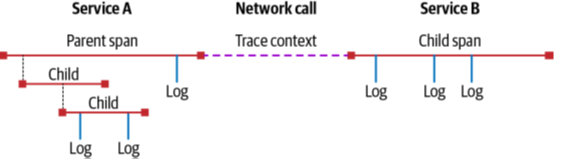
\includegraphics[width=1\textwidth]{resources/ch2/tracing-illus.png}
      \caption{Ilustrasi Tracing}
      \label{TracingIlllustration}
\end{figure}

Adapun komponen-komponen yang membangun sistem Distributed Tracing adalah sebagai berikut \citep{parker2020distributed}:
\begin{enumerate}
      \item Instrumentasi \\
            Distributed Tracing membutuhkan data \textit{trace} agar dapat bekerja.
            Data \textit{trace} dihasilkan dengan cara menginstrumentasikan proses-proses \textit{service} atau mentrasformasikan data telemetri yang sudah ada ke data \textit{trace}.
      \item \textit{Deployment} \\
            Setelah data \textit{trace} dihasilkan, kita perlu mengirimkan data tersebut ke suatu tempat.
            Melakukan \textit{deployment} pada sistem \textit{tracing} membutuhkan pemahaman dimana perangkat lunak kita dijalankan di \textit{server} dan bagaimana perangkat tersebut dijalankan.
            Agar dapat memaksimalkan kemampuan dari \textit{tracing} juga meminimalkan \textit{overhead} yang terjadi pada aplikasi, kita perlu memahami teknik yang cocok untuk melakukan deployment pada sistem Distributed Tracing yang akan kita gunakan.
      \item Penyampaian \textit{Value} \\
            Saat \textit{service} kita telah dapat menghasilkan data \textit{trace} dan kita telah memiliki infrastruktur yang diperlukan untuk mengolah data \textit{trace} tersebut, kita akan memerlukan kakas yang tepat untuk menggabungkan \textit{trace} dari berbagai \textit{service} dengan metadata lain seperti \textit{metrics} dan \textit{logs} untuk dapat menghasilkan \textit{value} yang berguna bagi proses \textit{debugging}, \textit{profiling}, dan \textit{monitoring} perangkat lunak terdistribusi.
\end{enumerate}

\subsection{\textit{Context Propagation}}

\subsection{\textit{Critical Path}}
\label{crit-path}

%\subsection{Komponen Distributed Tracing}
%
%\subsubsection{Instrumentasi}
%
%\subsubsection{\textit{Deployment}}
%
%\subsubsection{\textit{Value Delivery}}



%\subsection{Pelacakan \textit{request causality}}
%\label{bab2-dtracing-causality}

\section{gRPC}
gRPC adalah sebuah \textit{framework} Remote Procedure Call (RPC) Open Source berperforma tinggi yang dapat dijalankan di berbagai environment \citep{grpc}.
gRPC dapat secara efisien menghubungkan \textit{service} yang berada di dalam dan antara data center dengan berbagai dukungan untuk melakukan load balancing, tracing, pengecekan kesehatan, dan autentikasi.
gRPC juga dapat diaplikasikan pada server yang terdistribusi untuk menghubungkan berbagai perangkat mulai dari aplikasi mobile dan browser ke layanan backend.
Seperti RPC pada umumnya, gRPC memungkinkan \textit{service} yang terpisah untuk mengakses fungsi layaknya objek lokal. Ada beberapa skenario penggunaan utama dari gRPC:
\begin{enumerate}
	\item Menghubungkan service-service yang bersifat poliglot seperti dalam arsitektur Microservice.
	\item Menghubungkan perangkat mobile, browser client ke service backend.
	\item Menghasilkan library bagi sisi client yang efisien.
\end{enumerate}

Secara default, gRPC menggunakan Protocol Buffers sebagai Interface Definition Language (IDL) dan juga sebagai format pertukaran pesannya (walaupun juga bisa menggunakan JSON sebagai format pertukaran data).
Langkah pertama ketika menggunakan Protocol Buffers adalah dengan mendefinisikan struktur dari data yang ingin diserialisasi dalam sebuah file proto, yaitu sebuah file teks biasa yang memiliki ekstensi “.proto”.
Data dari Protocol Buffers distrukturkan sebagai messages yang masing-masing memiliki catatan mengenai data yang berbentuk pasangan name-value yang disebut dengan fields.
Berikut adalah contoh sederhana dari file proto:
\lstinputlisting[captionpos=b, caption={Contoh File Proto}]{codes/ch2/hello.proto}

Ketika struktur data sudah dibuat, kode Proto tersebut perlu di compile menggunakan kakas bernama protoc yang akan membuat akses data dalam bahsa pemrograman yang dipilih.
gRPC menggunakan protoc untuk menghasilkan kode dari file Proto berupa: kode gRPC bagi client dan server, dan juga kode Protocol Buffer biasa yang digunakan untuk melakukan populasi, serialisasi, dan kode untuk mendapatkan tipe pesan.

Adapun penggunaan gRPC pada sistem client dan server adalah sebagai berikut:
\begin{enumerate}
	\item Mendefinisikan service beserta method apa saja yang bisa dipanggil beserta parameter dan juga return type bagi masing-masing method.
	\item  Server akan mengimplementasi interface hasil kompilasi protoc yang berasal dari method-method yang didefinisikan pada file proto.
	\item Client akan memanggil method yang sudah didefinisikan pada server.
\end{enumerate}



%\section{Protokol Komunikasi Microservice}
%Pada subbab ini akan dijelaskan beberapa protokol komunikasi yang bisa digunakan dalam arsitektur Microsevice.
%\subsection{REST API}
%Representational State Transfer (REST) merupakan sebuah gaya arsitektur yang dibuat untuk mendesain sistem yang berjalan di World Wide Web.
%REST pertama kali diperkenalkan oleh Roy Thomas Fielding dalam disertasinya pada tahun 2005 yang berjudul \textit{Architectural Styles and the Design of Network-based Software Architectures}.
%Dalam mendesain arsitektur, REST mendefinisikan beberapa aturan yaitu skalabilitas antara komponen yang berinteraksi, antar muka yang seragam, \textit{deployment} yang independen bagi komponen, dan pembuatan arsitektur berlapis yang dapat memfasilitasi komponen untuk melakukan \textit{caching} agar dapat mengurangi \textit{latency}, memperkuat \textit{security}, dan mengenkapsulasi sistem \textit{legacy} \citep{rest}.
%
%Application Programming Interface (API) yang didesain berdasarkan prinsip-prinsip REST disebut dengan RESTful API.
%Ada dua konsep utama yang dipakai dalam mendesain REST API yaitu \textit{resources}, atau sumber daya, dan \textit{representations}, atau representasi \citep{restful-book}.
%Resource yang dimaksud dalam konteks RESTful API bisa berarti apa saja yang cukup penting untuk direferensi dan diakses sebagai API.
%Sebuah \textit{resource} biasanya sesuatu yang dapat disimpan dalam komputer seperti sebuah data yang disimpan dalam database ataupun sebuah hasil dari eksekusi algoritme.
%Satu-satunya batasan pada setiap \textit{resource} tersebut adalah setiap resource harus memiliki sebuah URL.
%Representasi sendiri menggambarkan bagaimana kondisi atau \textit{\textit{state}} saat \textit{resource} tersebut diakses.
%Contoh paling umum dari representasi  RESTful API adalah mentransportasikan \textit{resource} melalui protokol HTTP dan dalam bentuk data JSON.
%
%Dalam praktiknya, \textit{resource} sendiri tidak bisa diakses dengan sembarang cara.
%Dalam sistem RESTful API, client dan server berinteraksi dengan saling mengirim pesan yang mengikuti protokol yang sudah ditentukan sebelumnya, dalam hal ini adalah mengikuti semantik dari protokol HTTP itu sendiri.
%HTTP mendefinisikan delapan jenis pesan yang berbeda, namun ada empat yang paling sering digunakan, yaitu:
%\begin{enumerate}
%      \item GET \\
%            Dapatkan representasi dari sebuah \textit{resource}.
%      \item DELETE \\
%            Hapus \textit{resource} tersebut.
%      \item POST \\
%            Buat sebuah \textit{resource} berdasarkan representasi yang diberikan.
%      \item PUT \\
%            Gantikan \textit{state} dari \textit{resource} yang dimaksud sesuai dengan representasi yang diberikan.
%\end{enumerate}
%
%Dalam penggunaannya bagi komunikasi Microservice, RESTful API melalui HTTP masih menjadi pilihan yang paling banyak digunakan oleh developer menurut survey yang dilakukan oleh The Software House pada tahun 2020 \citep{tsh2020}.
%Walaupun adopsi nya sebagai protokol komunikasi Microservice cukup populer, namun ada beberapa kekurangan dari RESTful API \citep{web-service-article} yaitu:
%\begin{enumerate}
%      \item Tidak cocok untuk data dalam jumlah besar
%      \item Latency dan Overhead dalam pemrosesan request karena pengunaan protokol HTTP
%      \item	RESTful API memiliki ketergantungan tinggi pada Header untuk mengatur \textit{state}
%\end{enumerate}
%
%\subsection{GraphQL}
%GraphQL merupakan sebuah bahasa query dan manipulasi untuk API dan runtime untuk memenuhi query tersebut dengan data yang sudah ada \citep{graphql}.
%GraphQL dikembangkan oleh Facebook sebelum dirilis ke publik sebagai proyek Open Source pada tahun 2015.
%Pendekatan GraphQL dalam membuat API seringkali dikontraskan dengan metode pembuatan API yang sudah ada seperti REST.
%Perbedaan utama antara pendekatan GraphQL adalah cara menstrukturkan data yang diekspos ke API.
%REST melakukan penstrukturan data berdasarkan \textit{resource} sementara GraphQL menstrukturkan data lewat query yang dispesifikkan oleh pengguna seperti SQL.
%
%Sebuah layanan GraphQL dibuat dengan cara mendefinisikan tipe-tipe data pada masing-masing \textit{field}-nya kemudian menyediakan masing-masing fungsi untuk setiap \textit{field} pada tipe data tersebut.
%
%\lstinputlisting[captionpos=b, caption={Definisi Query Data}]{codes/ch2/example.graphql}
%
%\lstinputlisting[captionpos=b, caption={Fungsi Handler}]{codes/ch2/graphql-handler.js}
%
%Dari tipe data yang didefinisikan di atas, berikut adalah contoh query GraphQL beserta response-nya:
%
%\lstinputlisting[captionpos=b, caption={Query GraphQL}]{codes/ch2/query.graphql}
%
%\lstinputlisting[captionpos=b, caption={\textit{Response} GraphQL dalam JSON}]{codes/ch2/response.json}
%
%\subsection{gRPC}
%gRPC adalah sebuah \textit{framework} Remote Procedure Call (RPC) Open Source berperforma tinggi yang dapat dijalankan di berbagai environment \citep{grpc}.
%gRPC dapat secara efisien menghubungkan \textit{service} yang berada di dalam dan antara data center dengan berbagai dukungan untuk melakukan load balancing, tracing, pengecekan kesehatan, dan autentikasi.
%gRPC juga dapat diaplikasikan pada server yang terdistribusi untuk menghubungkan berbagai perangkat mulai dari aplikasi mobile dan browser ke layanan backend.
%Seperti RPC pada umumnya, gRPC memungkinkan \textit{service} yang terpisah untuk mengakses fungsi layaknya objek lokal. Ada beberapa skenario penggunaan utama dari gRPC:
%\begin{enumerate}
%      \item Menghubungkan service-service yang bersifat poliglot seperti dalam arsitektur Microservice.
%      \item Menghubungkan perangkat mobile, browser client ke service backend.
%      \item Menghasilkan library bagi sisi client yang efisien.
%\end{enumerate}
%
%Secara default, gRPC menggunakan Protocol Buffers sebagai Interface Definition Language (IDL) dan juga sebagai format pertukaran pesannya (walaupun juga bisa menggunakan JSON sebagai format pertukaran data).
%Langkah pertama ketika menggunakan Protocol Buffers adalah dengan mendefinisikan struktur dari data yang ingin diserialisasi dalam sebuah file proto, yaitu sebuah file teks biasa yang memiliki ekstensi “.proto”.
%Data dari Protocol Buffers distrukturkan sebagai messages yang masing-masing memiliki catatan mengenai data yang berbentuk pasangan name-value yang disebut dengan fields.
%Berikut adalah contoh sederhana dari file proto:
%\lstinputlisting[captionpos=b, caption={Contoh File Proto}]{codes/ch2/hello.proto}
%
%Ketika struktur data sudah dibuat, kode Proto tersebut perlu di compile menggunakan kakas bernama protoc yang akan membuat akses data dalam bahsa pemrograman yang dipilih.
%gRPC menggunakan protoc untuk menghasilkan kode dari file Proto berupa: kode gRPC bagi client dan server, dan juga kode Protocol Buffer biasa yang digunakan untuk melakukan populasi, serialisasi, dan kode untuk mendapatkan tipe pesan.
%
%Adapun penggunaan gRPC pada sistem client dan server adalah sebagai berikut:
%\begin{enumerate}
%      \item Mendefinisikan service beserta method apa saja yang bisa dipanggil beserta parameter dan juga return type bagi masing-masing method.
%      \item  Server akan mengimplementasi interface hasil kompilasi protoc yang berasal dari method-method yang didefinisikan pada file proto.
%      \item Client akan memanggil method yang sudah didefinisikan pada server.
%\end{enumerate}
%
%\subsection{WebSocket}



%\section{\textit{Observability} pada Sistem Terdistribusi}
%\label{bab2-observability}

\section{Kubernetes}
\subsection{Arsitektur Kubernetes}
Arsitektur Kubernetes terdiri atas dua macam node yaitu master node dan worker node.
Setiap cluster Kubernetes terdiri dari minimal satu buah worker node dan satu atau lebih worker node.
Master node akan mengatur semua worker node dan pod yang ada di dalam cluster.
Dalam environment production, biasanya master node akan berjalan di beberapa komputer dan cluster akan berjalan dengan beberapa node sehingga menyediakan sifat fault-tolerance dan high-availability \citep{kube-arch}.
Untuk mengakses cluster Kubernetes, pengguna akan menspesifikkan perintah kepada master node melalui aplikasi command line bernama kubectl dan master node akan menyesuaikan state yang diminta oleh pengguna dengan memberikan perintah kepada worker node yang tersedia seperti membuat pod baru.
Berikut adalah gambaran arsitektur Kubernetes:
\begin{figure}[htb]
      \centering
      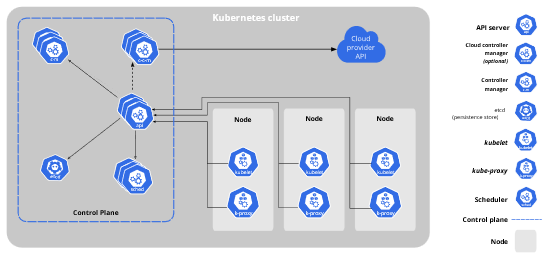
\includegraphics[width=0.9\textwidth]{resources/ch2/kube-1.png}
      \caption{Arsitektur Kubernetes \citep{kube-arch}}
      \label{KubeArch}
\end{figure}

Adapun komponen-komponen yang terdapat pada master node antara lain:
\begin{enumerate}
      \item Kube-apiserver adalah komponen dari master node yang mengekspos API Kubernetes. API Server adalah frontend dari worker node / control plane bagi Kubernetes.
      \item Etcd adalah komponen yang berfungsi sebagai penyimpan data yang konsisten dan higly-available dengan skema penyimpanan key-value.
      \item	Kube-scheduler berfungsi sebagai pengawas dan penjadwal bagi pod yang baru dibuat dan tugasnya adalah untuk menetapkan dimana node  bagi pod tersebut.
      \item	Kube-controller-manager adalah komponen yang berfungsi untuk menjalankan proses controller yaitu fungsi yang bertanggung jawab mengelola pod, worker node, dan mengatur tugas jika terjadi kegagalan pada proses pembuatan pod.
\end{enumerate}

Adapun komponen-komponen yang terdapat pada worker node antara lain:
\begin{enumerate}
      \item  Kubelet adalah komponen yang berfungsi sebagai agen di setiap node yang ada pada cluster dan bertugas untuk memastikan container yang berjalan pada pod.
      \item Kube-proxy adalah sebuah proxy jaringan yang berjalan di setiap node pada cluster dan mengimplementasikan konsep dari service Kubernetes.
      \item Container Runtime adalah sebuah perangkat lunak yang bertanggung jawab untuk menjalankan container. Kubernetes sendiri mendukung beberapa Container Runtime seperti Docker, containerd, CRI-O, dan semua jenis Runtime yang mengimplementasi Kubernetes CRI (Container Runtime Interface).
\end{enumerate}

\subsection{Pod}
Pod adalah unit terkecil yang dapat di deploy di dalam sebuah Kubernetes cluster.
Pod sendiri adalah sebuah abstraksi dari container yang di deploy di Kubernetes.
Jadi, ketika seorang pengguna ingin membuat sebuah aplikasi berbasis container di Kubernetes, pengguna tidak melakukan deploy container secara langsung melainkan melalui object Kubernetes yang bernama Pod.
Di dalam Pod sendiri bisa terdapat lebih dari satu buah container sekaligus sesuai dengan kebutuhan.
Contohnya ada jenis container yang disebut sebagai sidecar yang berfungsi sebagai secondary unit dari container utama yang ada di dalam Pod tersebut.
\subsection{Controller}
Kita bisa langsung membuat Pod di kubernetes lewat command line interface.
Namun jika kita membuat secara manual Pod, maka kita juga harus bertanggung jawab selama lifecycle dari Pod tersebut.
Masalah timbul ketika kita ingin membuat beberapa Pod yang sama sekaligus, maka akan menjadi suatu tugas yang tidak mudah untuk mengatur Pod-Pod tersebut.
Dari permasalahan itulah, ada sebuah konsep di Kubernetes yang disebut dengan Controller.

Controller adalah sebuah abstraksi di atas Pod yang bertugas untuk mengelola Pod secara otomatis dengan memanfaatkan komponen di dalam Pod yang bernama Container Probes.
Container Probes akan berfungsi untuk melakukan pengecekan apakah container yang berada di Pod berjalan dengan baik.
Jika Container Probes memberi tahu Controller bahwa container tidak berjalan dengan baik, maka Controller akan melakukan reset pada container tersebut.

Pada implementasinya, Kubernetes memiliki dua jenis implementasi dari Controller yaitu ReplicaSet dan DaemonSet.

\subsection{ReplicaSet}
ReplicaSet adalah jenis Controller yang bertanggung jawab untuk mengelola kebutuhan Pod sesuai state yang dispesifikkan oleh pengguna.
Cara ReplicaSet melakukan monitor pada Pod adalah melalui label yang telah ditetapkan ke sebuah Pod.
Jika label tersebut dengan selector yang terdapat pada ReplicaSet maka Pod akan masuk ke pengawasan dari ReplicaSet.
ReplicaSet akan mencocokkan keadaan Pod dengan spesifikasi yang diberikan oleh pengguna sehingga ketika ReplicaSet melihat bahwa Pod tidak sesuai dengan spesifikasi, contohnya banyaknya Pod tidak sesuai, ataupun satu node mati sehingga Pod yang ada di dalamnya terdampak, maka ReplicaSet akan menyesuaikan kondisi Pod tersebut.

\subsection{DaemonSet}
DaemonSet adalah jenis Controller yang memiliki fungsi untuk mengatur agar tepat ada satu Pod pada setiap node.
DaemonSet biasanya digunakan untuk mengelola Pod yang erat fungsinya dengan infrastruktur dari Kubernetes seperti mengatur jalannya operasi sistem, mengumpulkan log, atau memonitor resource di setiap node.

\subsection{Deployment}
Deployment adalah suatu abstraksi Controller di atas ReplicaSet yang tugasnya adalah melakukan deployment aplikasi Container di Kubernetes.
Deployment akan bekerja dengan mengatur ReplicaSet yang ada untuk mengatur pembaruan yang terjadi pada sebuah versi aplikasi Deployment.
Cara yang dilakukan oleh Deployment dalam mengatur versi aplikasi adalah dengan mengontrol ReplicaSet yang mengatur Pod.
Jika kita melakukan upgrade sebuah aplikasi pada Deployment, pertama kali Deployment akan menginstruksikan kepada ReplicaSet untuk mengurangi jumlah Pod yang diatur hingga nol.
Baru kemudian Deployment menginstruksikan kembali ReplicaSet untuk membuat Pod sebanyak spesifikasi.

Dengan fitur semacam itu, Deployment dapat memberikan fungsionalitas update tanpa adanya down time seperti melakukan rollback jika versi Deployment yang baru tidak sesuai yang diinginkan oleh pengguna.

\subsection{Service}
Fungsi networking adalah salah satu yang terpenting dalam sebuah sistem terdistribusi sebab suatu komponen perlu untuk berkomunikasi dengan komponen lainnya, dalam hal ini Pod.
Seperti yang sudah dipaparkan sebelumnya, Pod akan dikontrol oleh Controller, dalam hal ini adalah ReplicaSet melalui Deployment.
Dari sistem itu, ada kemungkinan bahwa Pod ynag berisi sebuah aplikasi container akan berubah sesuai yang dikehendaki oleh Controller-nya.
Jika kita melakukan komunikasi antar Pod langsung melalui IP address dari Pod tersebut, maka jika Pod tersebut hilang atau digantikan oleh Controller-nya maka IP address yang lama akan tidak bisa digunakan kembali.

Untuk menyelesaikan permasalahan tersebut, Kubernetes menggunakan sebuah layer abstraksi untuk Networking yang dinamakan Service.
Service akan menyediakan entry kepada sebuah Pod melalui Controller-nya, yaitu Deployment dan Service akan menyediakan IP address dan juga DNS entry yang tetap sehingga ketika Pod di dalam Deployment tersebut berubah, Pod akan tetap bisa diakses melalui Service.

Untuk memudahkan discovery dari sebuah Service, kubernetes memiliki sistem DNS nya sendiri yang diatur melalui master node.
Cara mengakses nya secara standar adalah jika pada sebuah Namespace yang sama, komponen Kubernetes yang lain dapat mengakses Service dan port nya langsung dengan format nama service itu sendiri.
Namun jika sebuah komponen Kubernetes lainnya mengakses Service tersebut dari luar Namespace tempat Service di deploy, maka cara pengaksesannya mengikuti format seperti berikut: \textit{[nama service].[namespace].svc.cluster.local}.

Dalam mengakomodasikan kebutuhan networking di Kubernetes, Service sendiri memiliki beberapa jenis yang dapat digunakan untuk berbagai usecase yang berbeda.
Tipe-tipe Service tersebut adalah:
\begin{enumerate}
      \item ClusterIP \\
            ClusterIP adalah tipe default dari Service. Seperti namanya, ClusterIP akan berbentuk sebuah IP address yang hanya bisa diakses dari dalam cluster dengan DNS.
      \item NodePort \\
            Dengan tipe Service ini, Kubernetes akan membuat sebuah port yang sama pada semua node yang dapat diakses dari luar cluster.
      \item LoadBalancer \\
            Tipe LoadBalancer adalah tipe Service khusus yang dipergunakan untuk mengekspos Service ke luar cluster melalui sebuah layanan Load Balancer. Layan Load Balancer yang dapat dipergunakan sendiri bisa dipilih sesuai dengan dimana cluster Kubernetes dibuat. Jika cluster dibuat di salah satu penyedia jasa Cloud Computing, maka LoadBalancer akan menggunakan layanan Load Balancer dari Cloud Computing tersebut untuk mengekspos Service ke luar cluster.
\end{enumerate}

\section{Database \textit{time-series}}

\section{Pendekatan untuk melakukan \textit{Performance Regression Analysis}}
Pada Subbab ini, akan dibahas beberapa pendekatan dan algoritme yang dapat digunakan untuk melakukan analisis pada regresi kinerja aplikasi berbasis Microservice.
\label{ch2-algo}
%\subsubsection{Integrasi dengan \textit{workflow} \textit{alerting}}


\subsection{Analisiis hasil \textit{Trace} individual}
Melihat hasil \textit{trace} individu adalah salah satu cara paling sederhana dalam memanfaatkan \textit{distributed tracing} sebagai bagian dari respon terhadap insiden dan analisis akar masalah \citep{parker2020distributed}. Hasil \textit{trace} individual dapat berguna terutama ketika kesalahan mudah diidentifikasi, seperti contohnya ada perubahan yang mengakibatkan kerusakan pada sebuah \textit{service}. Hal tersebut berarti semua \textit{request}, atau sebagian besar, gagal dalam eksekusinya, sehingga mudah untuk mengidentifikasi satu \textit{request} tersebut.

Risiko dari hanya menggunakan hasil \textit{trace} individual adalah karena perubahan dalam \textit{service} berjalan dengan cepat, akan sangat mungkin untuk menggeneralisir sebuah hasil \textit{trace} individual dan menyimpulkan penyebab yang salah dari sebuah insiden. 


%\subsubsection{Analisis sampel bias}


\subsection{Respons secara \textit{real-time}}
\label{approach-realtime}


\subsection{Analisis Kumulatif}
\label{approach-cumulative}

Salah satu cara untuk mengetahui kondisi metrik dari suatu sistem adalah dengan menggunakan histogram. Histogram sendiri adalah sebuah grafik yang menunjukkan perbandingan antara frekuensi kemunculan pada sumbu y dan metrik pada sumbu x. Artinya dengan histogram dapat ditunjukkan kondisi metrik dalam suatu sistem terdistribusi lewat tangkapan \textit{trace} secara keseluruhan. Salah satu metrik yang umum digunakan adalah latensi.

\begin{figure}[htb]
	\centering
	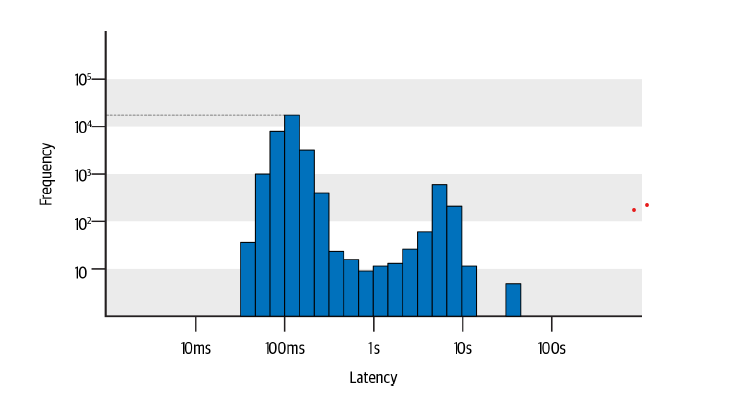
\includegraphics[width=1\textwidth]{resources/ch3/histogram-og.png}
	\caption{Contoh Histogram \citep{parker2020distributed}}
	\label{histogram}
\end{figure}

Ada beberapa teknik statistik yang dapat digunakan untuk mengetahui apakah dua buah sampel diambil dari sebuah distribusi yang sama. Salah satu teknik yang dapat digunakan adalah statistik Kolmogorov-Smirnov (K-S). Statistik K-S menghitung perbedaan dua buah distribusi sebagai sebuah bilangan skalar \citep{kolmogorov_1951}. Untuk mendapatkan distribusi tersebut, data yang berasal dari histogram akan terlebih dahulu diubah sebagai fungsi dengan fungsi distribusi kumulatif atau \textit{cumulative distribution function} (CDF). Ada dua perbedaan utama antara histogram dengan CDF. Pertama seperti namanya, CDF akan mengakumulasikan perhitungan, sehingga setiap titik pada CDF merupakan penjumlahan dari semua titik yang ada pada histogram di sebelah kiri. Kedua, sumbu y pada CDF dinormalisasi sehingga nilainya akan berkisar antara nol hingga satu. 

Gambar \ref{ks-example} menunjukkan dua buah CDF. Statistik K-S didapatkan dengan mencari jarak vertikal terjauh antara dua CDF seperti yang ditunjukkan oleh panah. Semakin besar jarak menunjukkan semakin mungkin bahwa dua buah CDF merupakan dua distribusi yang berbeda sehingga dapat menjadi indikasi bahwa terdapat perubahan pada kinerja. 

\begin{figure}[htb]
	\centering
	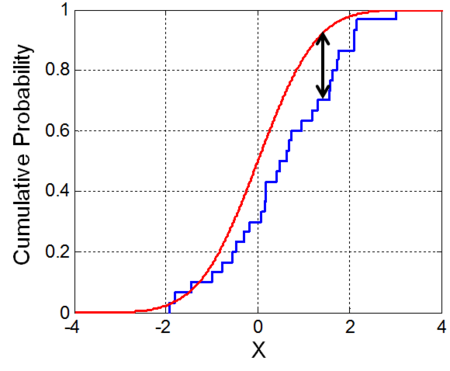
\includegraphics[width=0.6\textwidth]{resources/ch3/ks.png}
	\caption{CDF dari dua buah sampel, panah menunjukkan nilai statistik Kolmogorov-Smirnov \citep{wiki:ks-test}}
	\label{ks-example}
\end{figure}
%\subsection{Menentukan \textit{Critical Path}}b
%\label{approach-cp}
%Dalam setiap sistem terdistribusi yang cukup kompleks, selalu terdapat 

\subsection{Analisis Agregasi dan Korelasi}
\label{approach-corr}

Langkah pertama dalam menggunakan pendekatan ini adalah dengan membagi hasil \textit{trace} menjadi dua kelompok sampel, kedua jenis sampel ini akan menjadi basis bagi semua perbandingan kedepannya. Dengan asumsi regresi sudah diketahui terjadi, sampel bagian pertama harus berasal dari regresi itu sendiri. Hal tersebut mudah didapatkan jika regresi sedang terjadi sekarang. Jika regresi juga terjadi pada sebagian besar dari \textit{request}, maka sampel dari \textit{request} tersebut juga dapat menjadi penting. 

Bagian sampel kedua harus berasal dari kinerja \textit{baseline}. Hal tersebut dapat berasal dari sekumpulan \textit{trace} sebelum regeresi terjadi, mungkin dari satu jam, satu hari, atau bahkan satu minggu sebelumnya; artinya adalah pertama kali sekali, sistem \textit{tracing} harus memiliki terlebih dahulu catatan mengenai kinerja \textit{baseline} dari aplikasi. Catatan kinerja \textit{baseline} dapat diperoleh dari siklus penggunaan aplikasi oleh pengguna. Penggunaan alat visualisasi seperti histogram dapat dilakukan untuk mengidentifikasi sampel mana yang dapat menjadi representasi \textit{baseline} dari aplikasi.

Setelah dimiliki dua kelompok sampel (misal sampel A dan B) dan juga sekelompok fitur, analisis dilakukan dengan melihat setiap fitur dan mengajukan pertanyaan "Apa kemungkinan fitur tersebut ada pada sampel A tetapi tidak ada di sampel B?". Pertanyaan tersebut akan menghasilkan "koefisien korelasi" bagi setiap fitur. Koefisien yang bernilai 1.0 berarti sebuah fitur ada pada setiap \textit{trace} pada sampel A dan tidak pernah ada pada sebuah \textit{trace} di sampel B, sementara koefisien -1.0 berarti sebuah fitur yang ada pada setiap \textit{trace} di sampel B dan tidak pernah ada pada \textit{trace} di sampel A. Sebuah koefisien 0.0 berarti fitur tersebut secara seimbang dapat ada pada kedua sampel. Semakin dekat hasil ke 1.0 atau -1.0 sebuah koefisien korelasi, semakin mungkin sebuah fitur dapat menjelaskan perbedaan antara kedua sampel.

Metrik-metrik seperti \textit{latency}, \textit{error}, \textit{tag}, dan metadata lainnya dapat menjadi fitur yang berharga dari \textit{trace} yang dapat digunakan untuk memahami perubahan apa yang telah terjadi. Salah satu keunggulan dari penggunaan \textit{distributed tracing} adalah dapat menempatkan perubahan kinerja dalam konteks apa yang terjadi pada alur keberjalanan aplikasi. Ketika menentukan atribut apa dari \textit{trace} mana saja yang akan digunakan sebagai bagian dari analisis korelasi, harus diingat bahwa atribut tersebut haruslah berasal dari setiap \textit{span} pada \textit{trace} yang ada, bukan hanya yang terkait dengan sebuah \textit{service} tertentu.

Sebagai contoh, andaikan telah terjadi peningkatan \textit{latency} pada \textit{service} yang ada dan sebagai tindakannya kita membandingkan sampel \textit{trace} yang terjadi pada lima menit terakhir dengan sampel \textit{trace} yang terjadi pada satu jam yang lalu. Tabel \ref{corr-tab-1} menunjukkan sampel kecil dari fitur yang dapat diidentifikasi oleh analisis ini.

\begin{small}
	\begin{longtable}{ | p{10cm} | p{2cm} | }
			\caption{Contoh analisis korelasi}
			\label{corr-tab-1}                                                           
			\\ \hline
			\centering\bfseries{Fitur} & \centering\bfseries{Koefisien Korelasi} \tabularnewline \hline
			\endfirsthead
%			\hline
			\textbf{service}: inventory, \textbf{service.version}: 1.14.2 & 0.65 \\ \hline
			\textbf{runinfo.host}: vm73 & 0.41 \\ \hline
			\textbf{service}: inventory, \textbf{service.version}: 1.14.1 &  $\num{-0.65}$ \\ \hline
		\end{longtable}
\end{small}







\section{Penelitian Terkait}

%\subsection{Analisis Terotomasi dari \textit{Distributed Tracing}}
\subsection{Automated Analysis of Distributed Tracing}

\subsection{A Real-time Trace-level Root-cause Diagnosis System in Alibaba Datacenters}


\subsection{Dapper}

Dapper merupakan salah satu pionir teknologi \textit{distributed tracing} yang pertama kali dibuat oleh Google \citep{dapper-paper}. Dapper pertama kali dibuat untuk menyelesaikan permasalahan 

\subsection{Zipkin}

\subsection{Inkle}


%\chapter{Analisis Masalah dan Perancangan Solusi \textit{Performance Regression Analysis} menggunakan \textit{distributed tracing}}
\chapter{Analisis Masalah dan Perancangan Solusi}
%Pada bab ini diuraikan analisis persoalan pengumpulan data pada \textit{spreadsheet} yang telah diuraikan pada Bab I. Hasil dari bab ini digunakan untuk merancang kakas yang akan diimplementasikan seperti yang dijelaskan pada Bab IV.
%Berdasarkan 


\section{Analisis Masalah}

Seiring dengan meningkatnya kompleksitas dari aplikasi Microservice, seperti dengan meningkatnya jumlah service dan keterhubungan antar service yang ada di dalamnya, akan meningkat juga kompleksitas untuk melakukan \textit{monitoring} terhadap kinerja pada keseluruhan aplikasi Microservice. Salah satu isu penting terkait dengan kinerja adalah regresi atau penurunan terhadap kinerja. Kebutuhan untuk dengan segera menentukan penyebab utama dari regresi pada sistem menjadi penting apabila regresi terjadi pada lingkungan produksi yang langsung melayani \textit{request} dari pelanggan, sehingga apabila tidak diatasi dengan segera akan berdampak langsung terhadap pengalaman pengguna dalam menggunakan aplikasi. 

Terdapat dua pendekatan yang dapat dilakukan untuk mengatasi permasalahan regresi kinerja \citep{regression-detection}, yaitu:
\begin{enumerate}
	\item Deteksi regresi dilakukan setelah aplikasi selesai dikembangkan dan di-\textit{deploy} pada lingkungan terdedikasi
	\item Deteksi regresi dilakukan sebelum aplikasi selesai dikembangkan dan di-\textit{deploy} dan melakukan studi terhadap perubahan yang dihasilkan pada \textit{source code}
\end{enumerate}  

Mengingat sifat dari Microservice yang terdistribusi, akan menjadi sulit bagi \textit{developer} jika pendeteksian regresi dilakukan dengan pendekatan individual pada masing-masing service yang ada terlebih ketika jumlah service yang ada sudah sangat banyak dan hubungan interdependensi antar service menjadi rumit. Oleh karena itu, untuk mengatasi regresi kinerja pada aplikasi berbasis Microservice, dibutuhkanlah pendekatan yang tidak mengharuskan \textit{developer} untuk melakukan pencarian sumber masalah pada masing-masing service secara individu. Sehingga pada kasus deteksi dan analisis regresi kinerja aplikasi berbasis Microservice, pendekatan pertama lebih cocok untuk digunakan.

Salah satu teknologi yang dapat digunakan untuk melakukan \textit{monitoring} dan analisis regresi pada sebuah sistem terdistribusi seperti Microservice adalah \textit{distributed tracing}. Dengan bantuan mekanisme \textit{span} dari \textit{trace}, metrik-metrik kinerja dalam aplikasi berbasis Microservice dapat dilacak secara menyeluruh. Dalam kasus penggunaan seperti yang telah disebutkan sebelumnya, \textit{distributed tracing} cocok untuk digunakan dalam melakukan analisis regresi kinerja atau \textit{Performance Regression Analysis} dalam sebuah aplikasi berbasis Microservice sebab \textit{developer} tidak perlu menganalisis satu per satu \textit{service} yang ada terutama setelah \textit{service} sudah di-\textit{deploy}.

%Salah satu teknologi yang dapat menyediakan \textit{developer} kakas untuk melakukan \textit{monitoring} sebuah sistem terdistribusi secara keseluruhan adalah \textit{distributed tracing}. Dengan memanfaat

Oleh karena itu, dapat dirumuskan alur kerja yang harus dilakukan oleh sistem \textit{Performance Regression Analysis} (PRA) sebagai berikut:
\begin{enumerate}
	\item Sistem harus dapat mendeteksi ketika terjadi regresi pada aplikasi berbasis Microservice
	\item Sistem harus dapat menentukan sumber atau akar permasalahan dari regresi setelah terdeteksi
\end{enumerate}

%Untuk dapat melakukan 

%Adapun, langkah-langkah berikut dapat dilakukan untuk melakukan analisis penyebab regresi kinerja pada Microservice \citep{parker2020distributed}:
%\begin{enumerate}
%	\item Tentukan \textit{baseline} atau pengukuran dasar dari beberapa kinerja service
%	\item Ten
%\end{enumerate}

Sudah terdapat beberapa pendekatan yang dapat digunakan untuk melakukan analisis regresi seperti yang ada pada subbab \ref{ch2-algo}. Melihat kebutuhan dari sistem PRA di atas, dari beberapa pendekatan yang ada pada subbab tersebut, penulis menilai ada dua pendekatan yang dapat digunakan yaitu pendekatan Analisis Kumulatif pada \ref{approach-cumulative} dan pendekatan Analisis Agregasi dan Korelasi pada \ref{approach-corr}. Analisis Kumulatif dapat digunakan untuk menentukan apakah telah terjadi regresi pada aplikasi dengan melakukan perbandingan antara CDF \textit{baseline} dengan CDF dari aplikasi yang sedang berjalan. Ketika didapatkan statistik K-S yang melebihi \textit{threshold}, sistem PRA akan melakukan analisis akar permasalahan dengan metode Analisis Agregasi dan Korelasi untuk mendapatkan penyebab dari regresi melalui analisis \textit{crtical path} pada \textit{service} yang terdeteksi memiliki koefisien korelasi tinggi. Penghitungan koefisien korelasi dapat dilakukan dengan menghitung koefisien korelasi antara hasil \textit{trace} ketika terdeteksi regresi dengan hasil \textit{trace} dari \textit{baseline}.

Gambar \ref{alur-pra} menggambarkan fase yang akan dilakukan oleh sistem PRA. Secara umum, akan terdapat dua fase yang akan dilakukan yaitu fase \textit{baseline loading phase} dan fase \textit{realtime analysis phase}. Fase pertama yaitu \textit{loading} akan mencari data dari aktivitas aplikasi yang bersifat stabil yang dapat digunakan sebagai \textit{baseline} atau acuan bagi analisis yang akan dilakukan pada tahap selanjutnya. Fase ini akan menghasilkan dua buah artifak yaitu fungsi \textit{cumulative distribution function} (CDF) dari histogram hasil \textit{trace} dan juga data operasi yang terjadi pada \textit{critical path} semua \textit{span} beserta nilai \textit{latency}-nya yang akan disimpan sebagai pasangan \textit{key-value}. Fase berikutnya adalah fase analis secara \textit{realtime} yang akan membandingkan hasil transformasi CDF histogram \textit{span} yang sedang berlangsung sekarang dengan CDF \textit{baseline} hasil fase sebelumnya. Perbandingan tersebut akan dilakukan dalam periode tertentu. Untuk perancangan awal, periode waktu yang digunakan adalah selama 10 menit sekali. Perbandingan dari kedua CDF tadi akan menghasilkan statistik Kolmogorov-Smirnov (K-S). Jika statistik K-S yang dihasilkan melebihi batas \textit{threshold}, maka dapat disimpulkan bahwa terjadi regresi pada periode \textit{capture} histogram tersebut. 

\begin{figure}[htb]
	\centering
	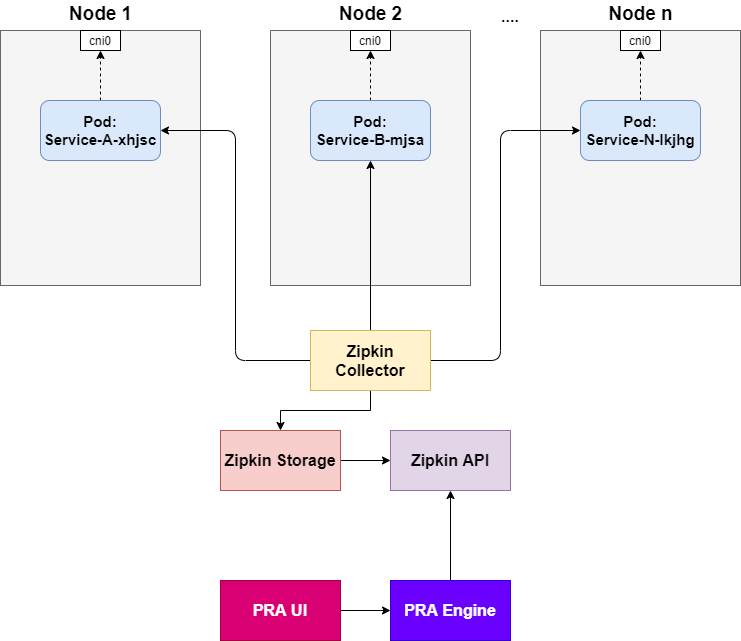
\includegraphics[width=1\textwidth]{resources/ch3/alur.png}
	\caption{Alur sistem \textit{Performance Regression Analysis}}
	\label{alur-pra}
\end{figure}

%Melihat kebutuhan untuk melakukan deteksi regresi secara terdistribusi pada Microservice, penulis menilai bahwa \textit{distributed tracing} dapat digunakan sebagai solusi untuk menyelesaikan masalah tersebut. Beberapa 


%ketika terjadi penurunan pada kinerja ataupun terdapat \textit{error} yang diakibatkan oleh suatu service tertentu.
%
%
%Regresi dalam sebuah sistem terdistribusi dapat diakibatkan oleh beberapa hal, contohnya adalah 
%\section{Analisis Alternatif Solusi} %Ngebandingin 

\section{Rancangan Solusi}

\subsection{Desain \textit{Payload}}

\subsection{Aristektur Solusi}

%\section{Rancangan Pengukuran \textit{Overhead}} % Di Bab 4

 \section{Jadwal Pelaksanaan}
 \newsavebox\mybox
 \begin{lrbox}{\mybox}
	     \begin{ganttchart}[
		     vgrid={*{6}{draw=none}, dotted},
		     x unit=.05cm,
		     y unit title=.6cm,
		     y unit chart=.6cm,
		     time slot format=isodate,
		     time slot format/start date=2016-09-01]{2021-09-01}{2022-04-30}
		     \ganttset{bar height=.6}
		     \gantttitlecalendar{year, month} \\
		     \ganttbar[bar/.append style={fill=blue}]{Studi Literatur}{2021-09-01}{2021-11-30}\\
		     \ganttbar[bar/.append style={fill=blue}]{Analisis Masalah}{2021-10-01}{2021-11-15}\\
		     \ganttbar[bar/.append style={fill=blue}]{Perancangan Solusi}{2021-11-01}{2021-12-15}\\
		     \ganttbar[bar/.append style={fill=blue}]{Implementasi}{2021-12-15}{2022-03-01}\\
		     \ganttbar[bar/.append style={fill=blue}]{Pengujian dan Analisis Hasil}{2022-02-01}{2022-04-30}
		     \end{ganttchart}
	 \end{lrbox}

 Pengerjaan tugas akhir ini direncanakan mulai pada September 2021 sampai April 2022. Pelaksanaan tugas akhir ini dibagi menjadi 5 tahap yang dapat dipetakan kepada metodologi pengerjaan sebagai berikut,
 \begin{enumerate}
	     \item Tahap 1: Studi Literatur
	     \item Tahap 2: Analisis Masalah
	     \item Tahap 3: Perancangan Solusi
	     \item Tahap 4: Implementasi
	     \item Tahap 5: Pengujian dan Analisis Hasil
	 \end{enumerate}
 Jadwal pelaksanaan tugas akhir berdasarkan metodologi pengerjaan tugas akhir dapat dilihat pada Tabel \ref{Gantt-Chart} dibawah ini.
 \begin{table}[htb]
	 \centering
	 \caption{Gantt Chart jadwal pelaksanaan tugas akhir}
	 \label{Gantt-Chart}
	 \tikz{
		   \node[inner sep=0pt,outer sep=0pt] (gantt)
		   {\begin{tabular}{c}
				     \toprule
				     \resizebox{\textwidth}{!}{\usebox\mybox} \\
				     \bottomrule
				    \end{tabular}%
			    };
		 }   
	 \end{table}

% Pada masa sebelum adopsi arsitektur Microservice dan kebanyakan dari aplikasi masih menggunakan arsitektur Monolith, proses seperti \textit{debugging} adalah hal yang sederhana sebab jika terdapat suatu \textit{error} akan mudah untuk ditelusuri dari mana asal \textit{error} tersebut sebab hanya ada satu aplikasi yang digunakan. Hal tersebut tidak berlaku jika aplikasi menggunakan model Sistem Terdistribusi, salah satu contohnya adalah Microservice. Sifat dari Microservice yang melakukan \textit{decoupling} aplikasi menjadi bagian yang lebih kecil membuat proses \textit{debugging} menjadi tidak mudah sebab untuk mencari penyebab \textit{error} aplikasi yang terdistribusi, kita harus mengetahui terlebih dahulu sumber dari \textit{error} tersebut. Kompleksitas akan bertambah dalam proses debugging jika ternyata ditemukan bahwa sautu \textit{error} pada sebuah \textit{service} bukanlah akar atau penyebab utama dari \textit{error} tersebut melainkan suatu \textit{service} lainnya. Kompleksitas akan bertambah jika metode \textit{debugging} yang digunakan mengharuskan \textit{developer} yang menangani \textit{error} tersebut harus menelusuri satu per satu \textit{service} yang terdampak sampai menemukan akar dari masalahnya. Dari masalah tersebutlah timbul suatu kebutuhan untuk mendapatkan gambaran mengenai \textit{state} sebuah Sistem Terdistribusi ataupun yang disebut juga dengan \textit{observability}.
% 
% 
% 
% Dengan bantuan dari \textit{trace} atau yang disebut \textit{distributed tracing}, \textit{developer} bisa mendapatkan suatu gambaran dari masing-masing \textit{request} yang terjadi pada sebuah \textit{resource} atau komponen yang berinteraksi dengan komponen lainnya dalam sebuah Sistem Terdistribusi seperti \textit{node}, \textit{service}, \textit{network}, ataupun \textit{mutex}. Ide dasar dari \textit{tracing} seperti yang sudah dijelaskan pada \ref{bab2-dtracing} adalah dengan mengidentifikasi sebuah titik spesifik, dapat jadi sebuah pemanggilan \textit{remote procedure call} (RPC), dalam sebuah aplikasi, \textit{library}, ataupun \textit{middleware} dalam jalur sebuah \textit{request} yang merepresentasikan kedua hal berikut:
% \begin{enumerate}
% \item \textit{Fork} pada eksekusi di level Sistem Operasi
% \item Sebuah lompatan atau akses horizontal ke luar melalui jaringan
%\end{enumerate}
%
%Data hasil \textit{trace} yang berisi kumpulan \textit{span} kemudian direpresentasikan sebagai \textit{directed acylic graph} (DAG), yang mana \textit{edge} antar graf dalam DAG yang disebut dengan \textit{reference} merepresentasikan hubungan atau kausalitas antar komponen dalam sebuah \textit{cluster} sistem terdistribusi yang terjadi pada \textit{request}. 
%
%
%
%Dengan meningkatkan performa \textit{baseline} pada sistem, para \textit{developer} berharap dapat meningkatkan kepuasan pelanggan, menurunkan biaya infrastruktur, ataupun keduanya. Untuk aplikasi yang langsung melayani pelanggan, performa seringkali berarti \textit{latency} dari \textit{request}. Proses optimisasi seperti ini biasanya adalah proses bertahap yang membutuhkan waktu.
%
%Kakas yang digunakan untuk membantu mencapai \textit{observability} penting untuk meningkatkan performa \textit{baseline} dengan pertama kali mengukur performa awal yang menjadi \textit{baseline} pengukuran dan digunakan untuk mengarahkan para \textit{developer} agar dapat mencari bagian mana dari aplikasi yang dapat ditingkatkan performanya. Dengan aplikasi yang menggunakan arsitektur Monolith, para \textit{developer} dapat dengan mudah melakukan \textit{profiling} proses mana saja yang dapat ditingkatkan penggunaan \textit{resource}-nya seperti CPU ataupun Memory. Namun dengan penggunaan arsitektur Microservice yang berbasis sistem terdistribusi, terkadang sulit untuk mengetahui \textit{service} manakah yang tepatnya perlu ditingkatkan penggunaan \textit{resource}-nya, sehingga penggunaan \textit{distributed tracing} akan sangat membantu untuk meningkatkan performa \textit{baseline} dari sebuah sistem terdistribusi.
%
%Berbeda dengan tujuan untuk meningkatkan performa \textit{baseline}, tujuan lainnya yaitu untuk mengembalikan performa \textit{baseline} bukanlah suatu hal yang dapat begitu saja direncanakan. Regresi dalam performa dapat muncul tiba-tiba seperti terjadinya \textit{outtage} atau pemberhentian tiba-tiba dari sebuah \textit{cluster} sistem terdistribusi. Melihat sifat dari sistem terdistribusi, mencari penyebab utama dari sebuah \textit{outtage} bukanlah sebuah hal yang mudah terlebih jika ada ratusan bahkan ribuan \textit{node} yang terdapat pada \textit{cluster} dan masing-masing \textit{node} saling terhubung dengan yang lainnya. Jika hal semacam tersebut terjadi dalam lingkungan aplikasi \textit{production} maka dampaknya akan terasa langsung oleh pelanggan dan dalam jangka panjang dapat menimbulkan kerugian material. Oleh karena itu, penting untuk segera mengetahui sumber atau akar dari suatu kejadian yang menyebabkan regresi pada performa sistem.
%
%Dari solusi \textit{distributed tracing} bersifat \textit{open source} yang tersedia saat ini, Zipkin dan Jaeger adalah dua solusi \textit{tracing} yang sudah menyediakan komponen instrumentasi, \textit{deployment}, dan \textit{value delivery} dalam bentuk \textit{application programming interface} (API) dan \textit{user interface} secara \textit{default}. Berikut adalah tabel perbandingan dari fitur \textit{user interface} web Zipkin dan Jaeger.
%
%
%\begin{small}
%	\begin{longtable}{ | p{3.75cm} | p{5.5cm} | p{5.5cm} | }
%		\caption{Deskripsi Perbandingan fitur Zipkin dan Jaeger}
%		\label{jzipkin-comparison}                                                                                                                \\ \hline
%		 & \centering\bfseries{Jaeger \citep{jaeger}} & \centering\bfseries{Zipkin \citep{zipkin}} \tabularnewline \hline
%		\endfirsthead
%		\bfseries{Deskripsi Singkat} & Dirilis sebagai kakas \textit{open-source} oleh Uber Technologies. Jaeger digunakan untuk melakukan \textit{monitoring} dan \textit{troubleshoot} dari sistem terdistribusi yang berbasis Microservice & Membantu mengumpulkan data bersifat temporal yang dibutuhkan untuk melakukan \textit{troubleshoot} permasalahn \textit{latency} pada aplikasi Microservice. Zipkin mengatur pengoleksian dan juga pencarian data. Desain dari Zipkin dibuat berdasarkan \textit{paper} dari Daper \citep{dapper-paper}\\ \hline
%		\bfseries{Kelebihan} &  \textit{Open-source}; 
%		Siap digunakan dengan Docker; Antarmuka dari \textit{collector} cocok digunakan dengan protokol milik Zipkin; Tingkat \textit{sampling} yang bersifat dinamis; Memiliki antarmuka berbasis Web &  \textit{Open-source}; 
%		Siap digunakan dengan Docker; Dapat menggunakan teknologi transport bagi \textit{span} yang berbeda-beda (HTTP, Kafka, Scribe, AMQP); Memiliki antar muka berbasis Web  \\ \hline
%		\bfseries{Kekurangan} & Hanya mendukung dua teknologi transport untuk \textit{span} (Thrift dan HTTP) & Tingkat \textit{sampling} yang bersifat \textit{fixed} \\ \hline
%		\bfseries{Jenis Analisis tersedia} & Visualisasi graf dependensi; Perbandingan hasil \textit{trace} & Visualisasi graf dependensi \\ \hline
%	\end{longtable}
%\end{small}
%
%Dari pemaparan mengenai kedua tujuan dari \textit{observability} di atas dan berdasarkan studi terhadap solusi \textit{open-source} yang sudah ada, penulis menyimpulkan bahwa ada dua hal yang dapat dibuat dengan menggunakan \textit{distributed tracing} untuk mencapai kedua tujuan utama dari \textit{observability}:
%\begin{enumerate}
%	\item Membuat Service Map untuk mencapai tujuan pertama yaitu meningkatkan performa baseline
%	\item Membuat perangkat untuk melakukan Root Cause Analysis (RCA) untuk mencapai tujuan kedua yaitu mengembalikan performa baseline ketika terjadi regresi pada sistem
%\end{enumerate}
%
%Service Map merupakan visualisasi dari sebuah sistem Microservice yang melakukan dekomposisi pada semua komponen \textit{service} dan menggambarkan dependensi yang terlihat antar \textit{service} tersebut secara \textit{real-time}, sehingga \textit{developer} dapat mengidentifikasi \textit{bottleneck} yang ada dan memahami bagaimana data mengalir dalam aristektur \citep{datadog-svcmap}. Untuk dapat membantu meningkatkan performa \textit{baseline}, sebuah Service Map harus dapat menyediakan informasi mengenai hubungan interdependensi antara \textit{service}, jumlah \textit{request} yang diterima oleh service per satuan waktu, dan ukuran performa pada \textit{service} tersebut dalam merespon \textit{service} lainnya. Ukuran performa yang dapat dijadikan \textit{baseline} antara lain adalah \textit{latency}, \textit{failure rate}, \textit{traffic rate}, dan saturasi, namun biasanya \textit{developer} hanya berfokus pada pengukuran \textit{latency} dan \textit{failure rate} \citep{parker2020distributed}.
%
%Selain digunakan untuk mendapatkan gambaran mengenai komponen yang ada pada suatu \textit{cluster} sistem terdistribusi, salah satu pendekatan yang dapat digunakan oleh Service Map untuk meningkatkan performa \textit{baseline}  disebut \textit{Correlation Analysis} \citep{parker2020distributed}. Untuk melakukan \textit{Correlation Analysis}, dibutuhkan tidak hanya satu tetapi dua sampel dari \textit{trace}. Satu sampel harus dapat merepresentasikan kelas \textit{trace} yang hendak dieliminasi atau setidaknya dikurangi jumlahnya, contohnya \textit{request} yang gagal atau lambat. Sampel jenis kedua harus dapat merepresentasikan komplemen dari sampel yang pertama, biasanya sekelompok \textit{request} yang cepat atau sukses. Selain dari dua kelompok sampel tadi, dibutuhkan juga sekelompok fitur yang dapat dicari korelasinya. Fitur-fitur yang dicari dalam sebuah sistem terdistribusi antara lain adalah \textit{service}, operasi, \textit{error}, dan \textit{tag} yang berasosiasi dengan \textit{span} yang membuat \textit{trace} tersebut. 
%
%Setelah dimiliki dua kelompok sampel (misal sampel A dan B) dan juga sekelompok fitur, analisis dilakukan dengan melihat setiap fitur dan mengajukan pertanyaan "Apa kemungkinan fitur tersebut ada pada sampel A tetapi tidak ada di sampel B?". Pertanyaan tersebut akan menghasilkan "koefisien korelasi" bagi setiap fitur. Koefisien yang bernilai 1.0 berarti sebuah fitur ada pada setiap \textit{trace} pada sampel A dan tidak pernah ada pada sebuah \textit{trace} di sampel B, sementara koefisien -1.0 berarti sebuah fitur yang ada pada setiap \textit{trace} di sampel B dan tidak pernah ada pada \textit{trace} di sampel A. Sebuah koefisien 0.0 berarti fitur tersebut secara seimbang dapat ada pada kedua sampel. Semakin dekat hasil ke 1.0 atau -1.0 sebuah koefisien korelasi, semakin mungkin sebuah fitur dapat menjelaskan perbedaan antara kedua sampel. 
%
%Di sisi lain, kakas untuk melakukan Root Cause Analysis dapat digunakan untuk memberikan petunjuk kepada \textit{developer} mengenai komponen mana dari Microservice yang mengalami regresi sehingga \textit{developer} dapat mengatasi permasalahan tersebut dengan segera. Salah satu pendekatan yang bisa dilakukan untuk mengembalikan performa adalah dengan pendekatan \textit{Aggregate and Correlation Root Cause Analysis} \citep{parker2020distributed}. Tidak jauh berbeda dengan pendekatan yang telah terlebih dahulu disebutkan pada Service Map, pendekatan ini menggunakan agregasi dari beberapa \textit{trace} untuk mendapatkan koefisien korelasi mengenai keadaan performa sebuah \textit{service}. 
%
%Adapun dari pemaparan di atas mengenai fitur analisis \textit{distributed tracing}, penulis menyimpulkan kebutuhan fungsional apa saja yang diperlukan pada pembuatan kakas visualisasi \textit{distributed tracing}:
%
%\begin{small}
%	\begin{longtable}{ | p{2cm} | p{10cm} | }
%		\caption{Kebutuhan Fungsional kakas visualisasi}
%		\label{fr-vis}                                                                                                                     \\ \hline
%		\centering\bfseries{ID} & \centering\bfseries{Deskripsi} \tabularnewline \hline
%		\endfirsthead
%		\hline
%		\centering\bfseries{ID} & \centering\bfseries{Deskripsi} \tabularnewline \hline
%		\endhead
%		FR-01 & Kakas dapt menampilkan hubungan interdependensi antara \textit{service} \\ \hline
%		FR-02 & Kakas dapat menampilkan pengukuran performa \textit{latency} pada setiap \textit{service} \\ \hline
%		FR-03 & Kakas dapat melakukan \textit{Correlation Analysis} untuk menentukan komponen mana dari Microservice yang dapat ditingkatkan performanya \\ \hline
%		FR-04 & Kakas dapat melakukan Root Cause Analysis (RCA) ketika terjadi sebuah regresi pada sistem dengan menggunakan pendekatan \textit{Aggregate and Correlation Root Cause Analysis} \\ \hline
%	\end{longtable}
%\end{small}






%Untuk mencapai kedua tujuan dari \textit{observability} tersebut, \textit{distributed tracing} dapat digunakan untuk menyediakan hal-hal berikut:
%\begin{enumerate}
%	\item 
%\end{enumerate}



%Seiring dengan meningkatnya penggunaan arsitektur, mengingkat pula kebutuhan bagi para \textit{developer} untuk dapat dengan segera mengetahui sumber dari permasalahan jika terjadi \textit{error} pada sistem.
%
%Dari pemaparan mengenai masih kurangnya kakas visualisasi \textit{tracing} yang bersifat \textit{open source}
%. Berdasarkan studi literatur mengenai \textit{observability} untuk Sistem Terdistribusi pada \ref{bab2-observability}, terdapat 

%Isu visualisasi 
%Overhead



\chapter{Implementasi dan Pengujian}

Bab ini akan membahas seluruh proses implementasi yang dilakukan untuk menerapkan rancangan yang sudah didefinisikan sebelumnya. Selain itu, bab ini juga akan membahas pengujian yang dilakukan terhadap hasil implementasi yang mencakup hal-hal yang diuji, metode pengujian, dan hasil pengujian yang diperoleh. 


\section{Implementasi}
Implementasi sistem \textit{Performance Regression Analysis} (PRA) akan dibuat berdasarkan rancangan arsitektur seperti yang terdapat pada gambar \ref{arch-pra}. Komponen seperti \textit{library} instrumentasi, melainkan akan melakukan \textit{fork} dan modifikasi solusi \textit{Open Source} \textit{distributed tracing} dari Zipkin. Komponen yang akan dibuat dari awal sepenuhnya adalah komponen PRA \textit{User Interface} (UI) dan PRA Engine dari sistem PRA yang akan melakukan komputasi utama sistem pendeteksian dan analisis regresi. Komponen PRA Engine juga akan berfungsi sebagai API yang akan diakses oleh komponen PRA UI.



\subsection{Implementasi PRA Engine}

Sebelum melakukan implementasi solusi, penulis harus terlebih dahulu melakukan pemilihan kakas yang akan digunakan melakukan implementasinya. Secara umum, terdapat banyak bahasa pemrograman yang dapat melakukan implementasi solusi komponeasdn \textit{engine} sesuai dengan alur yang terdapat pada gambar \ref{alur-pra}. Namun, ada suatu kebutuhan penting untuk melakukan tes statistik Kolmogorov-Smirnov (K-S) yang tidak semua bahasa pemrograman memiliki dukungan \textit{library} untuk melakukannya. Terdapat dua bahasa pemrograman yang memiliki \textit{library} untuk melakukan tes K-S yaitu bahasa pemrograman \textbf{Go} dan \textbf{Python}. Bahasa \textbf{Go} memiliki library Gonum \footnote{\url{gonum.org}} yang memiliki implementasi tes K-S dalam fungsi \texttt{KolmogorovSmirnov}, sementara bahasa \textbf{Python} memiliki library SciPy \footnote{\url{scipy.org}} yang memiliki implementasi tes K-S dalam fungsi \texttt{scipy.stat.ks\textunderscore 2samp}.

Dari kedua bahasa tersebut, penulis memilih bahasa \textbf{Python} untuk melakukan implementasi solusi setelah berhasil melakukan \textit{parsing} data \textit{trace} Zipkin dengan pendekatan pemrograman berorientasi objek yang didasarkan pada \textit{source code} yang dimiliki oleh aplikasi \textit{User Interface} milik Zipkin yang diimplementasikan menggunakan bahasa \textbf{Javascript}. 

Implementasi \textit{engine} akan terbagi menjadi beberapa modul seperti yang terlihat pada tabel \ref{engine-module}.

\begin{small}
	\begin{longtable}{ | p{1cm} | p{3cm} | p{10cm} | }
		\caption{Tabel pembagian modul komponen \textit{engine}}
		\label{engine-module}                                                           
		\\ \hline
		\centering\bfseries{ID} & \centering\bfseries{Nama Modul} & \centering\bfseries{Deskripsi} \tabularnewline \hline
		\endfirsthead
		EM-1 & zipkin (Pengambilan Data) & Modul ini bertanggung jawab untuk mengambil data dari API Zipkin yang memiliki data hasil \textit{trace} dari aplikasi. \\ \hline
		EM-2 & transform (Transformasi Data) & Modul ini bertanggung jawab untuk melakukan transformasi dari data \textit{trace} mentah yang diambil dari API Zipkin menjadi bentuk-bentuk model yang akan digunakan untuk komputasi di tahap selanjutnya seperti sampel data \textit{latency}, dan model data \textit{Critical Path}. Semua model akan disimpan dalam data berbentuk JSON. \\ \hline
		EM-3 & storage (Penyimpanan Data) & Modul ini bertanggung jawab untuk menyimpan model hasil transformasi \textit{baseline} dari modul EM-2 ke \textit{storage} untuk digunakan kembali pada fase \textit{Periodical Analysis}. Komponen \textit{storage} yang akan digunakan adalah Redis. Alasan utama pemilihan Redis sebagai komponen \textit{storage} adalah Redis telah memiliki modul penyimpanan data dalam bentuk JSON dan memiliki kinerja yang tinggi sebab data disimpan secara \textit{in-memory}. \\ \hline
		EM-4 & statistic (Perhitungan Statistik) & Modul ini bertanggung jawab untuk melakukan komputasi perhitungan statistik yang mencakup pendeteksian regresi dengan menghitung koefisien Kolmogorov-Smirnov seperti yang telah dijelaskan pada subbab \ref{approach-cumulative} menggunakan fungsi yang disediakan oleh library SciPy. \\ \hline
		EM-5 & critical\textunderscore path (Analisis \textit{Critical Path}) & Modul ini bertanggung jawab untuk melakukan analisis \textit{Critical Path} yang bertujuan untuk mencari penyebab regresi dengan mencari \textit{Critical Path} dari tiap \textit{service} dan melihat perbandingan \textit{latency} dari operasi tersebut dengan \textit{latency} yang telah direkam sebelumnya pada fase \textit{Baseline Loading}. Operasi yang selisih \textit{latency}-nya melebihi \textit{threshold} diduga kuat merupakan penyebab utama dari regresi yang terjadi. \\ \hline
		EM-6 & scheduling (\textit{Scheduling}) & Pada modul ini akan diimplentasikan \textit{job} atau pekerjaan utama yang akan digunakan untuk melakukan analisis regresi dengan menggunakan fungsi-fungsi yang telah diimplementasikan pada modul-modul sebelumnya dan juga bertanggung jawab melakukan penjadwalan \textit{job} tertentu selama interval yang ditentukan.  \\ \hline
	\end{longtable}
\end{small}

Aplikasi \textit{engine} akan dibuat sebagai REST API dan akan diimplementasikan menggunakan \textit{framework} FastAPI. Fungsionalitas \textit{engine} akan diekspos melalui REST API sehingga dapat digunakan baik oleh komponen UI maupun langsung melalui pemanggilan HTTP untuk keperluan pengujian. Beberapa \textit{endpoint} yang akan diimplementasikan terlihat pada tabel \ref{endpoints}.

\begin{small}
	\begin{longtable}{ | p{1cm} | p{2cm} | p{3.5cm} | p{7.5cm} | }
		\caption{Tabel \textit{endpoint} API \textit{engine}}
		\label{endpoints}                                                           
		\\ \hline
		\centering\bfseries{ID} & \centering\bfseries{Operasi HTTP} & \centering\bfseries{\textit{endpoint}} & \centering\bfseries{Deskripsi} \tabularnewline \hline
		\endfirsthead
		EP-1 & \centering{GET} & \centering\texttt{/state} & Data \textit{state} dari \textit{engine} yang akan berisikan informasi mengenai status pendeteksian regresi, pengecekan terakhir regresi, dan hasil analysis \textit{critical path} yang diduga menjadi penyebab regresi. \\ \hline
		EP-2 & \centering{POST} & \centering\texttt{/baseline} & Dengan \textit{endpoint} ini, \textit{user} dapat membuat \textit{engine} mengambil data \textit{baseline} baru dengan menyuplai informasi mengenai waktu mulai dan waktu selesai \textit{trace} di Zipkin beserta dengan batas banyaknya \textit{trace} yang akan diambil. \\ \hline
		EP-3 & \centering{DELETE} & \centering\texttt{/baseline} & \textit{Endpoint} ini akan menghapus informasi mengenai \textit{baseline} yang ada di data \textit{state}. \\ \hline	
		EP-4 & \centering{GET} & \centering\texttt{/analysis/range} & \textit{Endpoint} ini berfungsi untuk memicu \textit{engine} untuk melakukan analisis regresi dengan informasi waktu mulai dan waktu selesai trace yang disuplai oleh pengguna melalui \textit{query parameter}. API kemudian akan mengembalikan hasil analisis berupa apakah regresi terdeteksi beserta analisis \textit{critical path}. \\ \hline
		EP-5 & \centering{GET} & \centering\texttt{/analysis/periodical} & \textit{Endpoint} ini berfungsi untuk memicu \textit{engine} untuk melakukan analisis regresi dengan informasi waktu mulai dan waktu selesai trace yang telah ditentukan sebelumnya dan juga melakukan \textit{update} informasi state dengan hasil analisis regresi yang telah dilakukan. API kemudian akan mengembalikan hasil analisis berupa apakah regresi terdeteksi beserta analisis \textit{critical path}. \\ \hline				
	\end{longtable}
\end{small}

Secara umum, alur kerja endpoint EP-4 dan EP-5 serupa dengan perbedaan kecil waktu pengambilan \textit{trace} yang mana EP-4 dapat mengambil data \textit{trace} secara secara presisi dengan parameter waktu awal dan waktu akhir \textit{trace} sehingga endpoint ini akan digunakan untuk melakukan pengujian secara manual, sementara EP-5 digunakan untuk menyimulasikan tingkah laku dari \textit{engine} yang melakukan analisis dalam interval waktu tertentu tanpa harus menunggu interval waktunya.

Alur kerja analisis regresi pertama dimulai dengan mengambil data \textit{trace} yang akan dilakukan oleh modul EM-1. Data \textit{trace} akan diambil dari API Zipkin dalam bentuk JSON dan akan dilakukan \textit{parsing} sehingga data akhir yang didapatkan mengandung informasi \textit{latency} dari semua \textit{span} yang terdapat pada \textit{trace} tersebut. Setelah data \textit{trace} diambil dari API dan di-\textit{parse} oleh modul EM-1, selanjutnya data \textit{trace} tersebut akan ditransformasikan untuk diambil informasi \textit{latency}-nya oleh modul EM-2. Selanjutnya, dengan asumsi bahwa data \textit{baseline} telah didapatkan, \textit{engine} selanjutnya akan mengambil data \textit{latency} baseline yang akan dilakukan oleh modul EM-3. Setelah informasi \textit{latency} \textit{baseline} maupun periodikal sudah didapatkan, selanjutnya analisis pertama-tama dilakukan dengan menguji terjadinya regresi dengan fungsi statistik dari modul EM-4. Hasilnya adalah sebuah variabel \textit{boolean} yang melakukan tes K-S untuk menentukan apakah kedua sampel data tersebut berasal dari distribusi yang berbeda. Jika hasil tes menghasilkan kedua data berasal dari distribusi yang berbeda, dapat menjadi indikasi bahwa regresi telah terjadi. 

Jika terindikasi regresi telah terjadi, \textit{engine} selanjutnya akan melakukan analisis \textit{critical path}. Pertama-tama data \textit{trace} \textit{baseline} maupun periodikal akan ditransformasikan menjadi model \textit{critical path} oleh modul EM-2. Kemudian kedua model \textit{critical path} tersebut akan dibandingkan oleh modul EM-5 dan hasil akhirnya adalah data perbandingan operasi-operasi yang ada di data \textit{baseline} dan periodikal. Hasil akhir data pengecekan regresi dan analisis \textit{critical path} akan dikirim sebagai \textit{response} dalam bentuk JSON oleh API. Semua operasi dari alur kerja yang telah disebutkan di atas diimplementasikan dalam fungsi yang terdapat pada modul EM-6.

\subsubsection{Struktur implementasi}
Modul-modul pada tabel \ref{engine-module} masing-masing akan diimplementasikan sebagai \textit{package} pada bahasa \textbf{Python} seperti yang terlihat pada gambar \ref{package}. Terdapat tujuh buah \textit{package}, enam buah \textit{package} dari modul dan satu buah \textit{package} \texttt{utils} yang berisi fungsi-fungsi untuk mendukung kerja fungsi di modul lainnya. Semua \textit{source code} hasil implementasi disimpan di Github \footnote{\url{https://github.com/masterraf21/pra\textunderscore engine}}.
\begin{figure}[!htb]
	\centering
	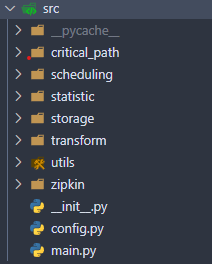
\includegraphics[width=0.35\textwidth]{resources/ch4/packages.png}
	\caption{Implementasi modul sebagai \textit{package}}
	\label{package}
\end{figure} 

%Gambar \ref{api_docs} adalah hasil tangkapan layar dokumentasi API yang disediakan oleh FastAPI. 
%\begin{figure}[!htb]
%	\centering
%	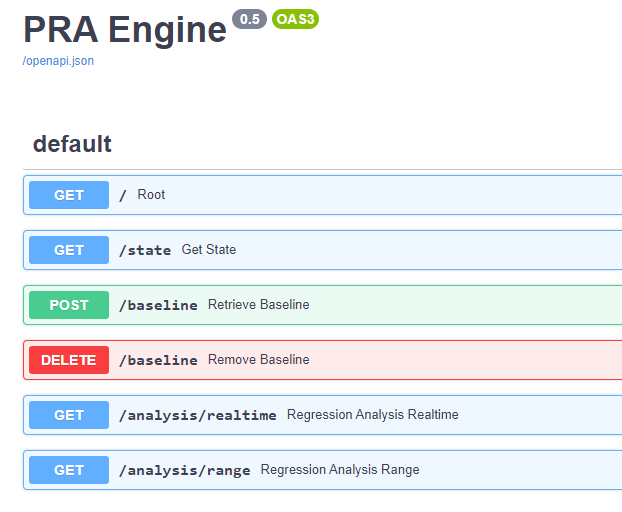
\includegraphics[width=0.5\textwidth]{resources/ch4/api_docs.png}
%	\caption{Dokumentasi API}
%	\label{api_docs}
%\end{figure} 
%
%Berikut adalah tangkapan layar dari hasil pemanggilan beberapa \textit{endpoint} yang dilakukan dengan aplikasi Postman \footnote{\url{https://www.postman.com/}}.
%\begin{figure}[h!]
%	\centering
%	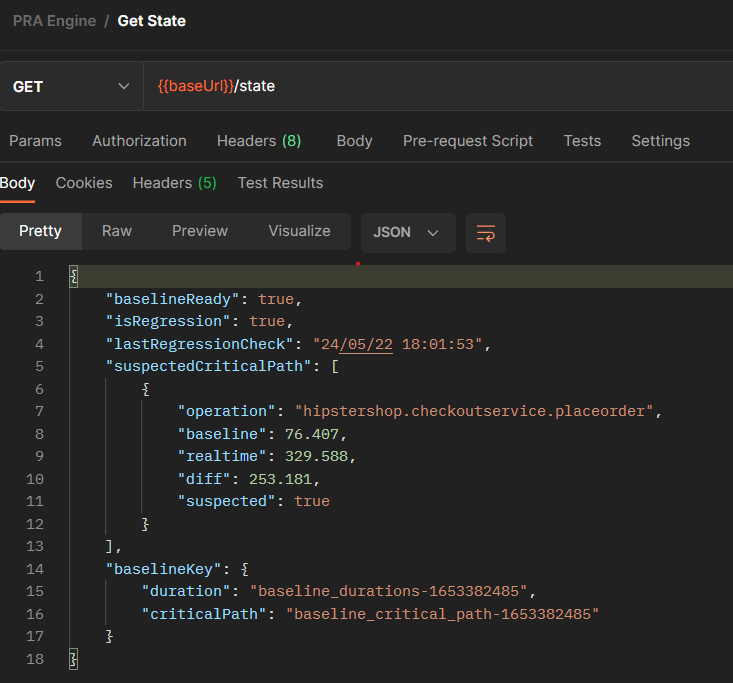
\includegraphics[width=0.75\textwidth]{resources/ch4/result_state.png}
%	\caption{Hasil pemanggilan \textit{endpoint} \texttt{/state}}
%	\label{api_state}
%\end{figure} 
%\begin{figure}[h!]
%	\centering
%	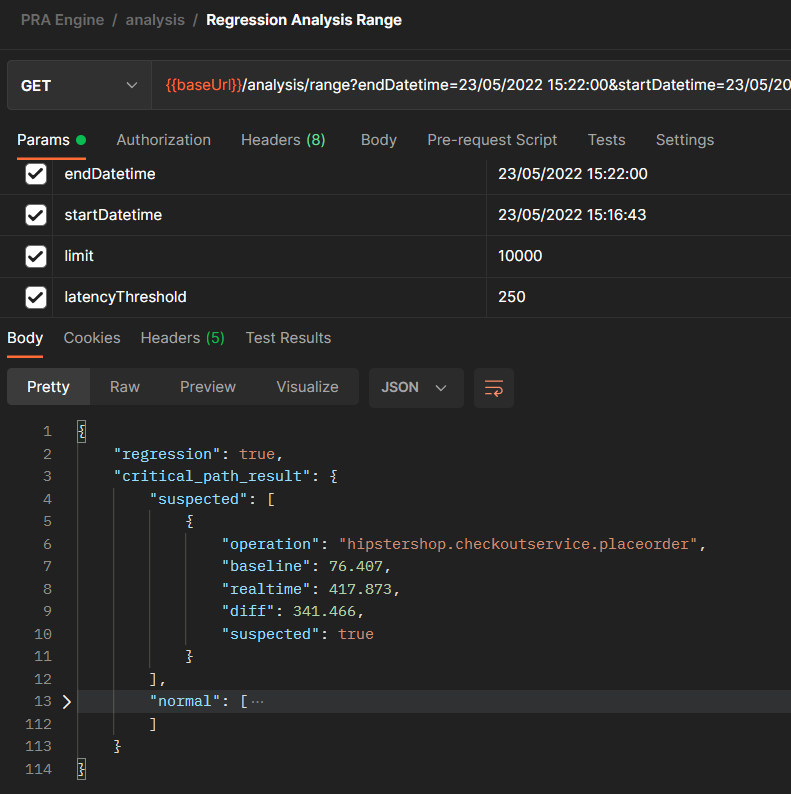
\includegraphics[width=0.75\textwidth]{resources/ch4/result_analysis_range.png}
%	\caption{Hasil pemanggilan \textit{endpoint} \texttt{/analysis/range}}
%	\label{api_analysis_range}
%\end{figure} 
%\begin{figure}[h!]
%	\centering
%	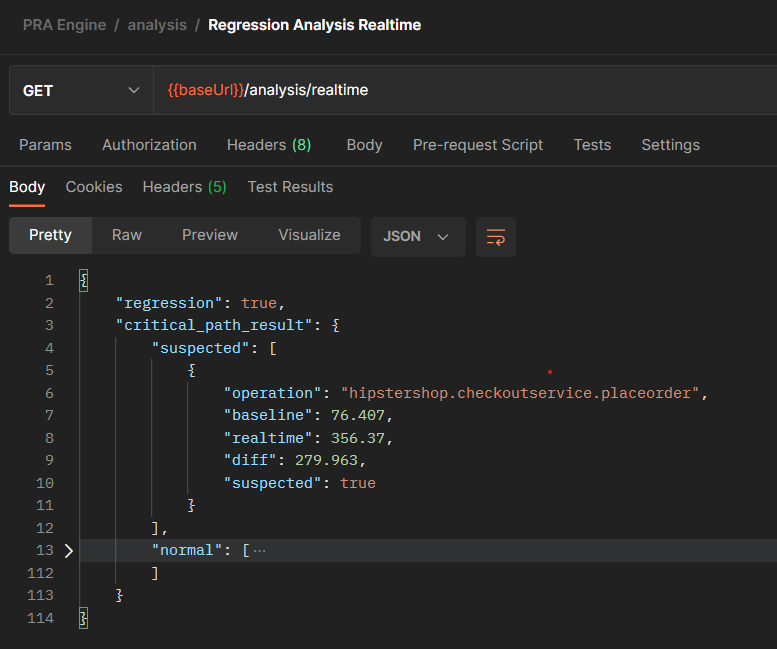
\includegraphics[width=0.75\textwidth]{resources/ch4/result_analysis_realtime.png}
%	\caption{Hasil pemanggilan \textit{endpoint} \texttt{/analysis/realtime}}
%	\label{api_analysis_realtime}
%\end{figure} 

\pagebreak


\subsubsection{Model dan Struktur Data}
Sistem PRA yang dibuat bergantung pada data \textit{trace} yang diperoleh dari Zipkin. Data tersebut tidak bisa begitu saja digunakan untuk menjalankan fungsi-fungsi dari \textit{engine} PRA sesuai yang terdapat pada gambar \ref{alur-pra} dan perlu ditransformasikan menjadi model dan struktur data yang lebih bermakna seperti yang telah disebutkan pada EM-2 di tabel \ref{engine-module}.

Dalam dokumentasinya, Zipkin menyediakan keterangan mengenai model data \textit{trace} yang digunakannya seperti yang terdapat pada \citep{zipkin-data}. Model data yang digunakan Zipkin terbagi menjadi dua yaitu \textit{span} dan \textit{trace}. \textit{Trace} sendiri merupakan serangkaian \textit{span} dengan id \textit{trace} sama yang merepresentasikan alur jalannya sebuah \textit{request} dalam sebuah \textit{service} yang telah terinstrumentasi, sementara \textit{span} merepresentasikan salah satu operasi yang terjadi sepanjang sebuah \textit{request}. Beberapa informasi yang terdapat pada data \textit{span} antara lain adalah informasi mengenai \textit{trace} dimana \textit{span} itu berada, metadata mengenai operasi yang direpresentasikan \textit{span}, durasi atau \textit{latency} dari operasi.

Sementara itu, untuk memenuhi fungsi-fungsi pada sistem PRA, data yang bersumber dari Zipkin perlu ditransformasikan menjadi struktur data yang sesuai dengan kebutuhan masing-masing tahap analisis. Dari rancangan alur sistem PRA, terdapat tiga tahap analisis yang akan dilakukan, yaitu tahap pendeteksian regresi dengan analisis statistik Kolmogorov-Smirnov, tahap analisis korelasi, dan tahap analisis \textit{critical path}.

Pada tahap pendeteksian regresi dengan tes statistik Kolmogorov-Smirnov (K-S), data yang diperlukan adalah data \textit{latency} atau durasi operasi dari \textit{span} yang dimiliki oleh Zipkin. Tes K-S akan membandingkan dua buah sampel data \textit{latency} dan akan menghasilkan hipotesis apakah kedua fungsi tersebut berada pada distribusi yang sama.

Pada tahap analisis \textit{critical path}, data yang dibutuhkan adalah pasangan \textit{key-value} dari nama operasi yang terrekam oleh Zipkin dan juga nilai \textit{latency} dari operasi tersebut. Data \textit{critical path} akan disimpan sebagai struktur data \textit{map} yang sesuai untuk menyimpan data berbentuk pasangan \textit{key-value}. Data ini akan didapatkan dari data \textit{trace} bawaan Zipkin yang sudah memiliki informasi mengenai \textit{critical path} dan juga nilai \textit{latency} nya masing-masing. 

\subsubsection{Algoritma}
Setelah pada subbab sebelumnya didefinisikan struktur data yang akan digunakan untuk merepresentasikan beberapa model seperti yang ada pada gambar \ref{alur-pra}, pada subbab ini akan didefinisikan algoritma penting yang akan digunakan untuk melakukan pendeteksian regresi pada aplikasi Microservice. 

algoritma yang didasarkan pada tes statistik Kolmogorov-Smirnov ini akan membandingkan dua buah sampel data dan akan menentukan apakah kedua sampel tersebut berasal dari distribusi yang sama. Pertama-tama kita definisikan dua hipotesis yaitu $h_{0}$ atau hipotesis \textit{null} yang menyatakan bahwa kedua sampel data berasal dari distribusi yang sama dan $h_{a}$ atau hipotesis alternatif yang menyatakan bahwa kedua sampel data berasal dari dua distribusi yang berbeda. 

Kemudian akan dijalankan tes statistik K-S yang dilakukan menggunakan fungsi dari \textit{library}
SciPy yang akan menghasilkan dua buah nilai, yaitu \texttt{statistic} dan \texttt{p-value}. Jika nilai \texttt{p-value} lebih kecil dari nilai signifikan, atau \texttt{alpha} pada fungsi,  maka kita dapat menolak $h_{0}$ dan menerima $h_{a}$. Jika  \texttt{p-value} tidak lebih kecil dari nilai signifikan, maka selanjutnya adalah membandingkan antara nilai \texttt{statistic} dan \texttt{critical value}. \texttt{Critical value} sendiri merupakan sebuah titik pada tes hipotesis yang akan dibandingkan pada hasil nilai \texttt{statistic} yang akan digunakan untuk menolak atau menerima hipotesis \textit{null}. Jika nilai \texttt{statistic} lebih besar dari nilai \texttt{critical value}, maka kita dapat menolak $h_{0}$ dan menerima $h_{a}$ atau artinya kedua sampel data berasal dari distribusi yang berbeda. Namun jika  nilai \texttt{statistic} lebih kecil dari nilai \texttt{critical value}, kita tidak dapat menolak $h_{0}$ atau artinya kedua sampel data berasal dari distribusi yang sama.


Jika kedua sampel ternyata berasal dari distribusi yang berbeda, maka dapat dicurigai telah terjadi regresi pada aplikasi sebab distribusi dari data yang bersumber dari  \textit{trace} periodikal berbeda dengan distribusi dari data \textit{trace} \textit{baseline} yang dijadikan acuan kinerja normal aplikasi.

\lstinputlisting[captionpos=b, language=Python,caption={Algoritma tes statistik Kolmogorov-Smirnov}]{codes/ch4/ks.py}


\subsection{Implementasi PRA UI}
Komponen lainnya yang akan diimplementasikan pada Tugas Akhir ini adalah komponen \textit{User Interface} (UI). Komponen ini akan menjadi antarmuka yang dapat digunakan untuk mengetahui \textit{state} dari sistem PRA. Fungsionalitas yang akan dibuat pada komponen UI akan dijabarkan pada tabel kebutuhan  fungsional \ref{ui-functional}.
\begin{small}
	\begin{longtable}{ | p{3cm} | p{9cm} | }
		\caption{Tabel kebutuhan fungsional komponen UI}
		\label{ui-functional}                                                           
		\\ \hline
		\centering\bfseries{ID} & \centering\bfseries{Deskripsi} \tabularnewline \hline
		\endfirsthead
		\centering{UI-1} & UI dapat menampilkan status pendeteksian regresi  \\ \hline
		\centering{UI-2} & UI dapat menampilkan hasil analisis \textit{critical path} berupa nama operasi dan nilai \textit{latency} \\ \hline

	\end{longtable}
\end{small}

\subsubsection{Hasil implementasi}
Berikut adalah tangkapan layar hasil implementasi komponen PRA UI.

\begin{figure}[!htb]
	\centering
	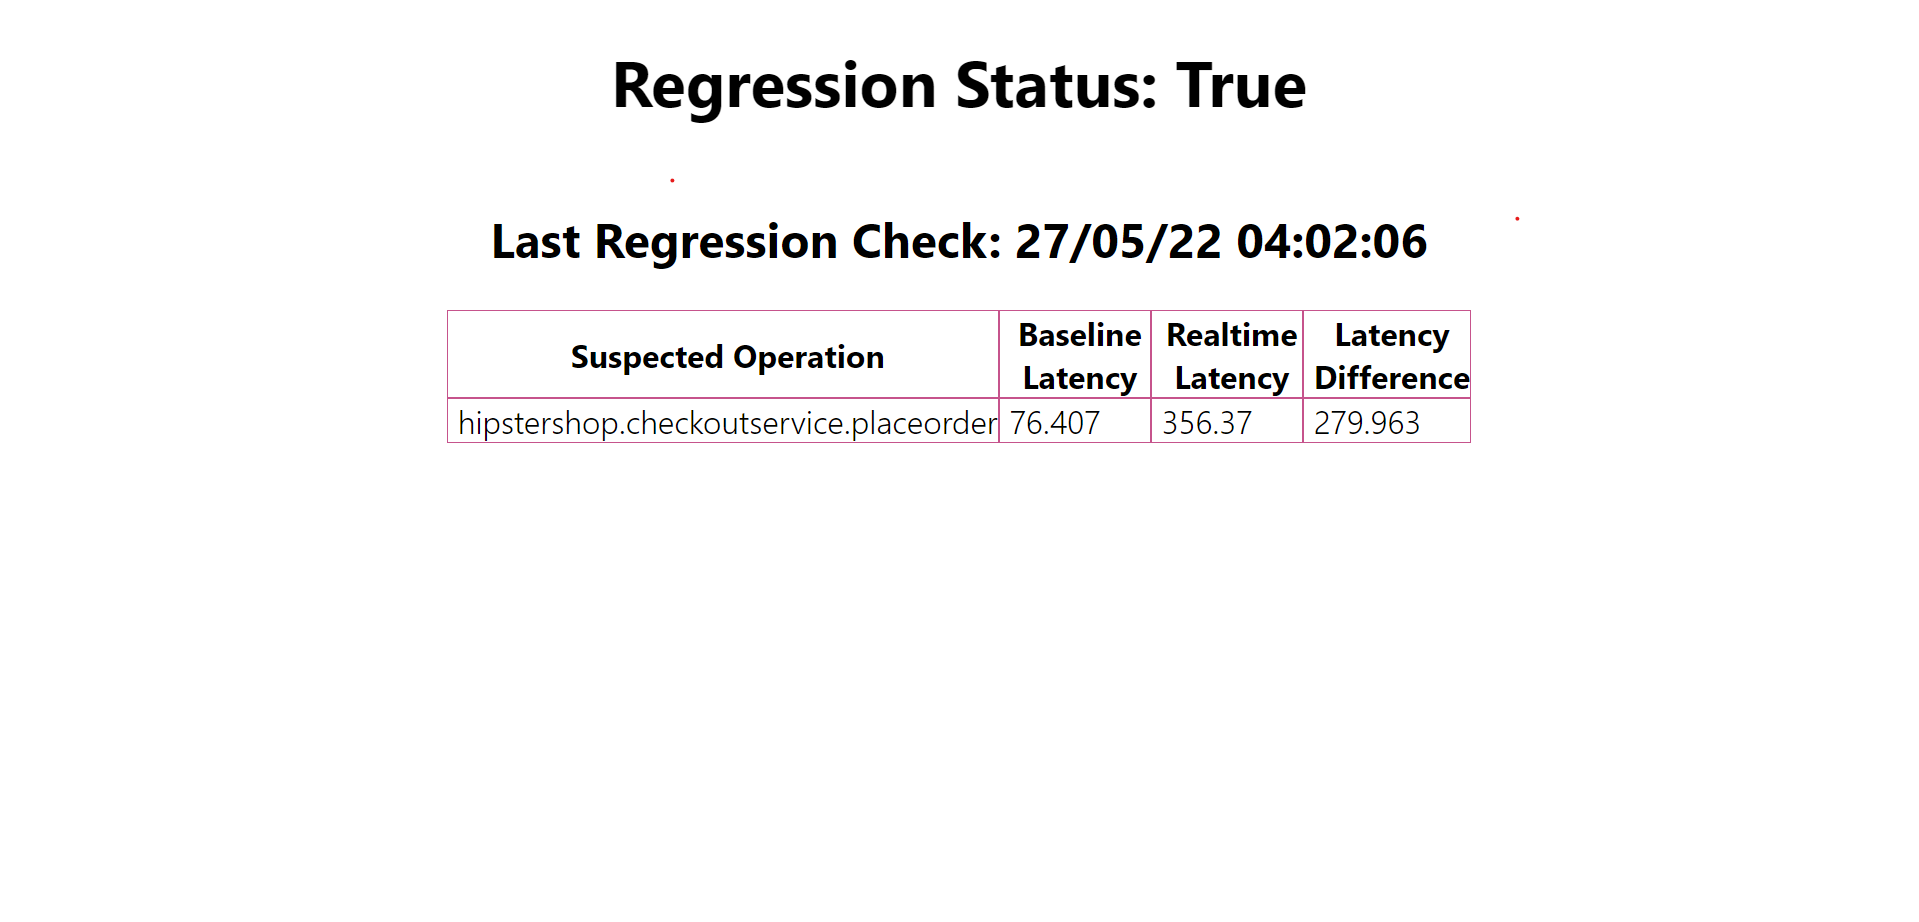
\includegraphics[width=1\textwidth]{resources/ch4/ui.png}
	\caption{Tangkapan layar UI}
	\label{ui}
\end{figure}

\section{Pengujian}
Untuk mengetahui keberhasilan dari sistem yang telah diimplementasikan, akan dilakukan pengujian sebagai berikut.
\subsection{Tujuan Pengujian}
Pengujian sistem PRA akan dilakukan dengan tujuan untuk:
\begin{enumerate}
	\item Mengukur keberhasilan sistem PRA dalam mendeteksi regresi
	\item Mengukur keberhasilan sistem PRA dalam menentukan kandidat sumber regresi
	\item Mengukur \textit{overhead} yang diakibatkan oleh sistem PRA dengan
	indikator berupa penggunaan memori dan pemanfaatan CPU.
\end{enumerate}

Tujuan utama pengujian sistem \textit{Performance Regression Analysis} adalah untuk menguji apakah sistem dapat mendeteksi terjadinya regresi atau penurunan kinerja dengan indikasi peningkatan nilai \textit{latency} yang disebabkan oleh perubahan yang terjadi pada aplikasi. Perubahan tersebut dapat berupa penambahan atau \textit{update} fitur, hasil perbaikan \textit{bug}, dsb. Sehingga kasus-kasus yang akan diujikan utamanya merupakan simulasi terjadinya perubahan pada level aplikasi \textit{microservice}. Namun sebagai perbandingan akan terdapat juga kasus-kasus yang menyimulasikan perubahan yang terjadi di luar level aplikasi seperti peningkatan jumlah pengguna dan peningkatan \textit{load} pada Load Generator pada \textit{service}-\textit{service} tertentu. Kasus pengujian akan dijelaskan lebih lanjut pada subbab \ref{metode-pengujian}.

\subsection{Lingkungan Pengujian}
Pengujian akan dilakukan pada Google Kubernetes Engine dengan spesifikasi yang dipaparkan pada tabel \ref{testing-env}.
\begin{small}
	\begin{longtable}{ | p{5cm} | p{8cm} | }
		\caption{Spesifikasi Lingkungan Pengujian}
		\label{testing-env}                                                           
		\\ \hline
		\centering\bfseries{Layanan Kubernetes} & \centering\bfseries{Google Kubernetes Engine} \tabularnewline \hline
		\endfirsthead
		\textit{Operating System} & Container Optimized OS (COS) \\ \hline
		\textit{Instance Type} & n1-standard-2 (2 vCPU,  7,5 GiB RAM) \\ \hline
		Jumlah Node & 3 \\ \hline
		
	\end{longtable}
\end{small}

\subsection{Aplikasi Pengujian}
Aplikasi yang akan digunakan untuk melakukan pengujian sistem PRA adalah aplikasi Hipster Shop yang merupakan aplikasi \textit{e-commerce} berbasis web yang dibuat untuk mendemostrasikan berbagai macam teknologi yang dimiliki oleh Google. Seperti pada gambar \ref{butiq-arch}, Hipster Shop terdiri atas 10 microservice yang saling berkomunikasi melalui gRPC. Selain itu Hipster Shop juga memiliki load generator yang secara terus menerus mengirimkan request untuk menyimulasikan alur belanja pengguna. Hipster Shop sudah memiliki load generator yang dibuat menggunakan Locust
untuk menyimulasikan pengunaan aplikasi oleh sejumlah user. Aplikasi Hipster Shop akan dimodifikasi dengan diinstumentasikan menggunakan Zipkin untuk menyimulasikan lingkungan \textit{distributed tracing} yang menggunakan Zipkin.
\begin{figure}[!htb]
	\centering
	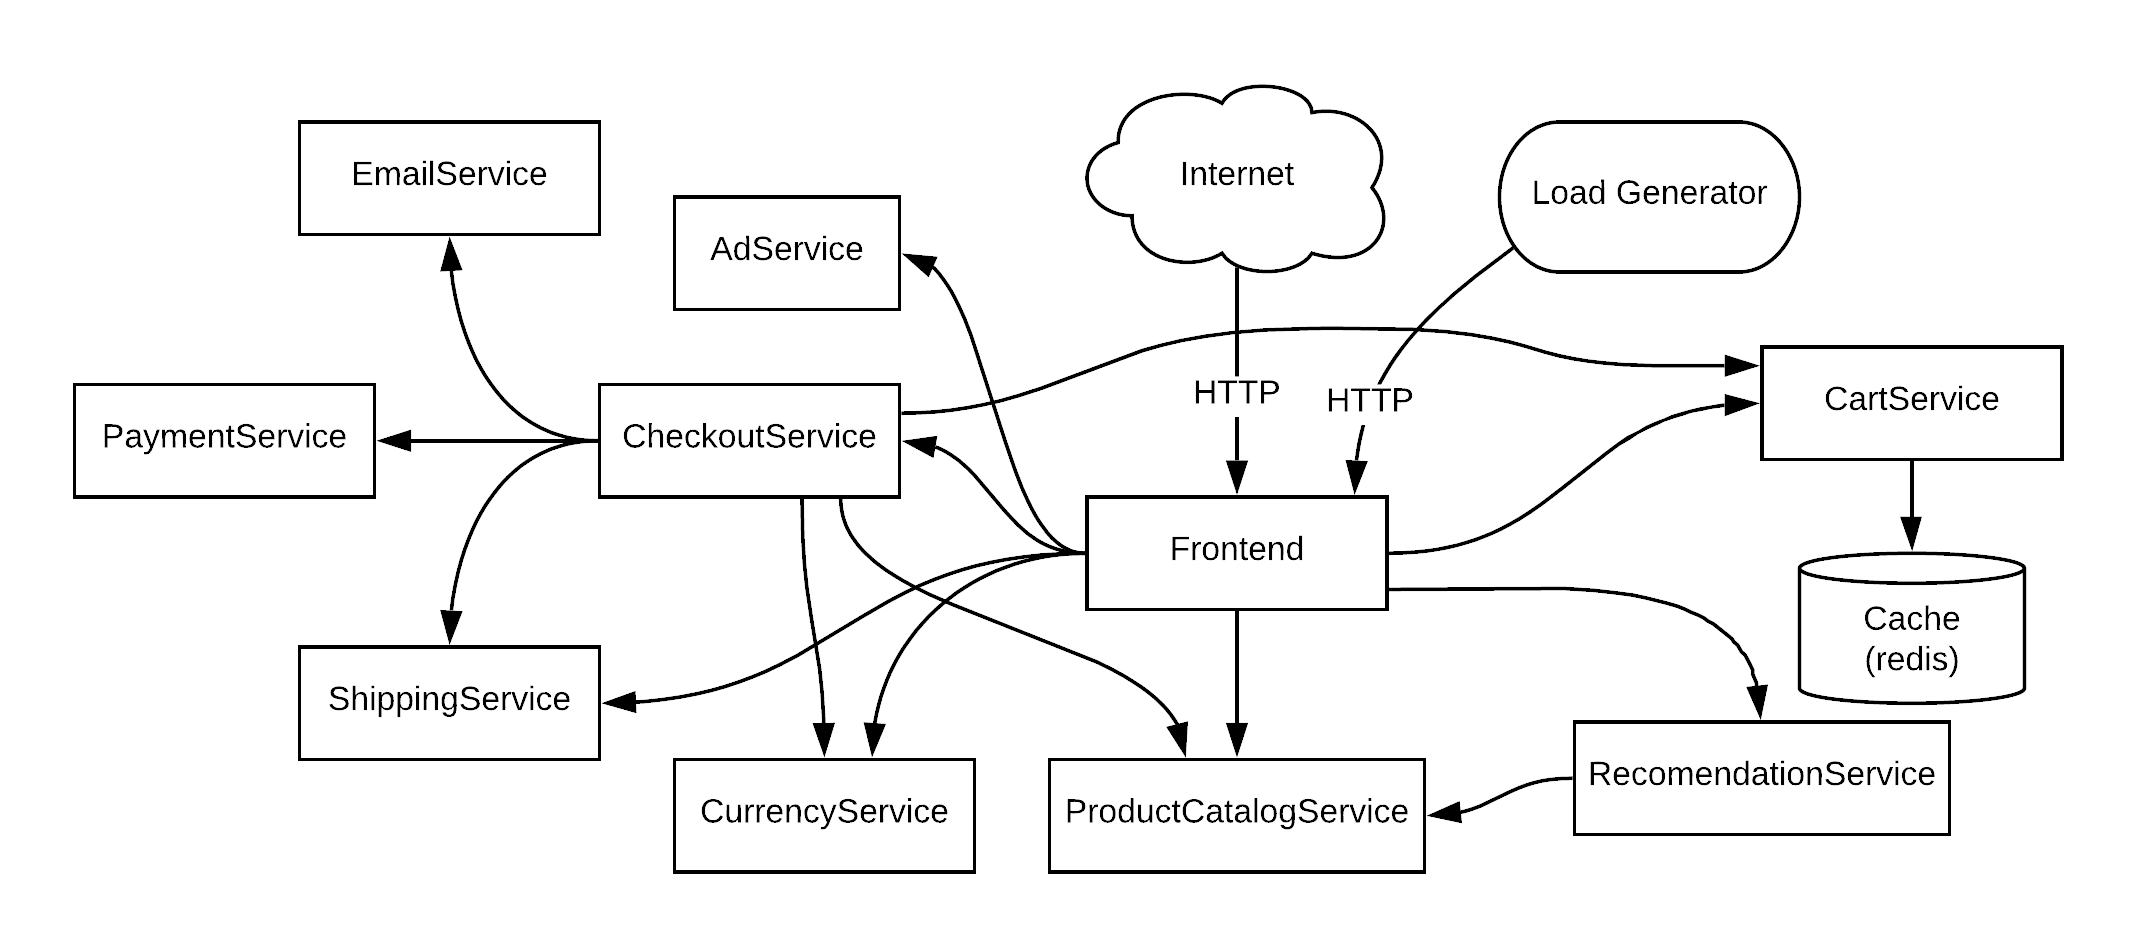
\includegraphics[width=1\textwidth]{resources/ch4/hipster-arch.png}
	\caption{Arsitektur aplikasi Hipster Shop}
	\label{butiq-arch}
\end{figure}

\pagebreak


\subsection{Metode Pengujian}
\label{metode-pengujian}
Untuk melakukan pengujian pada sistem PRA yang telah dibuat, \textit{service} yang ada pada Hipster Shop akan dimodifikasi untuk meniru perilaku dari \textit{service} yang mengalami regresi kinerja. Ada dua metode utama yang dapat dilakukan untuk membuat perilaku regresi pada \textit{service} yaitu dengan menambahkan perintah \textit{sleep} dan menambahkan \textit{loop} dengan operasi \textit{dereference} sebuah variabel yang membutuhkan banyak usaha dari CPU untuk menyelesaikannya sehingga diharapkan fungsi-fungsi tersebut akan memiliki \textit{latency} yang lebih besar. 

Ada dua tahap yang akan dilakukan untuk melakukan pengujian ini, pertama tahap pengambilan data \textit{baseline}. Data \textit{baseline} akan diambil dengan menyimulasikan pengunaan aplikasi dengan menggunakan Load Generator yang akan dijalankan dengan variabel \textbf{25 User} dan \textbf{5 Spawn Rate} selama \textbf{1 jam}. Data \textit{baseline} ini kemudian akan disimpan oleh \textit{engine} untuk dipergunakan di kasus-kasus pengujian selanjutnya. Tahap selanjutnya adalah melakukan pengujian dengan kasus-kasus yang akan dijelaskan lebih lanjut.

Terdapat dua jenis kasus uji yang akan diujikan pada sistem. Jenis pertama adalah kasus-kasus yang menyimulasikan regresi dengan melakukan perubahan yang terjadi di level aplikasi dengan cara melakukan modifikasi secara sengaja di level kode. Kasus pertama akan memiliki ID dengan awalan \textbf{SI} menandakan \textit{skenario-internal}. Jenis kedua adalah kasus-kasus yang menyimulasikan regresi dengan meningkatkan jumlah pengguna dan \textit{load} pada Load Generator. Kasus kedua akan memliki ID dengan awalan \textbf{SE} menandakan \textit{skenario-eksternal}. Tabel \ref{testcase} akan menjelaskan kasus-kasus pengujian sistem.

Pengujian pada tabel \ref{testcase} seluruhnya dilakukan dengan cara terlebih dahulu melakukan \textit{deployment} masing-masing kasus uji di lingkungan Kubernetes kemudian menjalankan aplikasi Load Generator sesuai dengan spesifikasi masing-masing kasus uji selama $\pm 5$ menit. Pengujian akan dilakukan dengan memanggil \textit{endpoint} \texttt{/analysis/range} dengan parameter StartTime dan EndTime yang sesuai dengan kasus uji. 

Untuk keperluan pengujian akan digunakan 3 level signifikan atau alpha yang berbeda yaitu 0,1, 0,05, dan 0,001. Ketiga level signifikan ini digunakan untuk mengetahui sensitivitas hasil pendeteksian regresi dengan arti semakin kecil nilai signifikan, maka akan semakin signifikan bukti untuk menolak $h_{0}$. Nilai signifikan 0,1 dipilih sebagai batas atas nilai signifikan untuk mengetahui tingkat sensitivitas dari kasus uji dengan nilai signifikan yang paling besar. Sementara nilai 0,05 dipilih sebab nilai tersebut merupakan nilai yang paling umum digunakan sebagai nilai signifikan pada tes statistik hipotesis. Sementara nilai 0,001 dipilih sebagai perbandingan nilai signifikan paling kecil untuk menguji batas bawah dari nilai signifikan.

Hasil akhir dari setiap kasus uji akan berupa \textit{response} dalam bentuk JSON dari API dan juga \textit{log} dari aplikasi untuk mengetahui hasil tes  statistik K-S yang akan dipergunakan untuk keperluan analisis selanjutnya.
\begin{table}[htb]
	\caption{Tabel kasus uji}
	
	\begin{adjustwidth}{-1.5cm}{}
		% Please add the following required packages to your document preamble:
		% \usepackage{multirow}
		% \usepackage[table,xcdraw]{xcolor}
		% If you use beamer only pass "xcolor=table" option, i.e. \documentclass[xcolor=table]{beamer}
		\begin{tabular}{llccl}
			\hline
			\rowcolor[HTML]{009901} 
			\multicolumn{1}{c}{\cellcolor[HTML]{009901}{\color[HTML]{FFFFFF} \textbf{ID}}} &
			\multicolumn{1}{c}{\cellcolor[HTML]{009901}{\color[HTML]{FFFFFF} \textbf{Service (Fungsi)}}} &
			\multicolumn{1}{l}{\cellcolor[HTML]{009901}{\color[HTML]{FFFFFF} \textbf{Extra Latency}}} &
			\multicolumn{1}{l}{\cellcolor[HTML]{009901}{\color[HTML]{FFFFFF} \textbf{User}}} &
			{\color[HTML]{FFFFFF} \textbf{Keterangan}} \\ \hline
			\multicolumn{1}{|l|}{\textbf{SI1}} &
			\multicolumn{1}{l|}{CheckoutService (placeorder)} &
			\multicolumn{1}{c|}{100ms} &
			\multicolumn{1}{c|}{25} &
			\multicolumn{1}{l|}{Kasus extra latency \#1} \\ \hline
			\multicolumn{1}{|l|}{\textbf{SI2}} &
			\multicolumn{1}{l|}{CheckoutService (placeorder)} &
			\multicolumn{1}{c|}{250ms} &
			\multicolumn{1}{c|}{25} &
			\multicolumn{1}{l|}{Kasus extra latency \#2} \\ \hline
			\multicolumn{1}{|l|}{\textbf{SI3}} &
			\multicolumn{1}{l|}{CheckoutService (placeorder)} &
			\multicolumn{1}{c|}{350ms} &
			\multicolumn{1}{c|}{25} &
			\multicolumn{1}{l|}{Kasus extra latency \#3} \\ \hline
			\multicolumn{1}{|l|}{\textbf{SI4}} &
			\multicolumn{1}{l|}{CheckoutService (placeorder)} &
			\multicolumn{1}{c|}{250ms} &
			\multicolumn{1}{c|}{75} &
			\multicolumn{1}{l|}{\begin{tabular}[c]{@{}l@{}}Kasus extra latency \\ dengan peningkatan user \#1\end{tabular}} \\ \hline
			\multicolumn{1}{|l|}{\textbf{SI5}} &
			\multicolumn{1}{l|}{CheckoutService (placeorder)} &
			\multicolumn{1}{c|}{250ms} &
			\multicolumn{1}{c|}{150} &
			\multicolumn{1}{l|}{\begin{tabular}[c]{@{}l@{}}Kasus extra latency \\ dengan peningkatan user \#1\end{tabular}} \\ \hline
			\multicolumn{1}{|l|}{\textbf{SI6}} &
			\multicolumn{1}{l|}{CheckoutService (placeorder)} &
			\multicolumn{1}{c|}{-} &
			\multicolumn{1}{c|}{25} &
			\multicolumn{1}{l|}{Kasus peningkatan kerja CPU} \\ \hline
			\multicolumn{1}{|l|}{} &
			\multicolumn{1}{l|}{CheckoutService (placeorder)} &
			\multicolumn{1}{c|}{} &
			\multicolumn{1}{c|}{} &
			\multicolumn{1}{l|}{} \\ \cline{2-2}
			\multicolumn{1}{|l|}{} &
			\multicolumn{1}{l|}{\begin{tabular}[c]{@{}l@{}}ProductCatalog (getproduct,\\ listproducts)\end{tabular}} &
			\multicolumn{1}{c|}{} &
			\multicolumn{1}{c|}{} &
			\multicolumn{1}{l|}{} \\ \cline{2-2}
			\multicolumn{1}{|l|}{} &
			\multicolumn{1}{l|}{ShippingService (getquote)} &
			\multicolumn{1}{c|}{} &
			\multicolumn{1}{c|}{} &
			\multicolumn{1}{l|}{} \\ \cline{2-2}
			\multicolumn{1}{|l|}{\multirow{-4}{*}{\textbf{SI7}}} &
			\multicolumn{1}{l|}{\begin{tabular}[c]{@{}l@{}}RecommendationService \\ (listrecommendations)\end{tabular}} &
			\multicolumn{1}{c|}{\multirow{-4}{*}{250ms}} &
			\multicolumn{1}{c|}{\multirow{-4}{*}{25}} &
			\multicolumn{1}{l|}{\multirow{-4}{*}{\begin{tabular}[c]{@{}l@{}}Kasus extra latency\\  dengan beberapa service\end{tabular}}} \\ \hline
			\multicolumn{1}{|l|}{\textbf{SE1}} &
			\multicolumn{1}{l|}{All Normal} &
			\multicolumn{1}{c|}{-} &
			\multicolumn{1}{c|}{75} &
			\multicolumn{1}{l|}{\begin{tabular}[c]{@{}l@{}}Tidak ada peningkatan latency\\ dengan peningkatan pengguna \#1\end{tabular}} \\ \hline
			\multicolumn{1}{|l|}{\textbf{SE2}} &
			\multicolumn{1}{l|}{All Normal} &
			\multicolumn{1}{c|}{-} &
			\multicolumn{1}{c|}{150} &
			\multicolumn{1}{l|}{\begin{tabular}[c]{@{}l@{}}Tidak ada peningkatan latency\\ dengan peningkatan pengguna \#1\end{tabular}} \\ \hline
			\multicolumn{1}{|l|}{\textbf{SE3}} &
			\multicolumn{1}{l|}{\begin{tabular}[c]{@{}l@{}}Checkout load \\ increased to 100 in loadgen\end{tabular}} &
			\multicolumn{1}{c|}{-} &
			\multicolumn{1}{c|}{25} &
			\multicolumn{1}{l|}{Tes pengujian load external \#1} \\ \hline
			\multicolumn{1}{|l|}{\textbf{SE4}} &
			\multicolumn{1}{l|}{\begin{tabular}[c]{@{}l@{}}Currency load\\  increased to 100 in loadgen\end{tabular}} &
			\multicolumn{1}{c|}{-} &
			\multicolumn{1}{c|}{25} &
			\multicolumn{1}{l|}{Tes pengujian load external \#2} \\ \hline
		\end{tabular}
	\end{adjustwidth}
	\label{testcase}
\end{table}
\pagebreak

\subsection{Hasil Pengujian Regresi}
Berikut adalah hasil pengujian yang telah dilakukan pada sistem PRA sesuai dengan kasus uji seperti yang telah dijabarkan pada tabel \ref{testcase}. Hasil tangkapan layar dari aplikasi Postman terdapat pada lampiran \ref{lampiran_a}.

\subsubsection{Kasus SI1}
Pada kasus ini di semua nilai alpha, regresi terdeteksi pada nilai alpha 0.1 namun tidak terdeteksi pada nilai alpha 0.05 dan 0.001. Analisis \textit{critical path} dapat menentukan sumber regresi pada nilai alpha 0.1 yaitu operasi \texttt{placeorder} dari \textit{service} \texttt{CheckoutService} dengan selisih perbedaan \textit{latency} sebesar 126ms.

\subsubsection{Kasus SI2}
Pada kasus ini di semua nilai alpha, regresi terdeteksi dan analisis \textit{critical path} dapat menentukan sumber regresi yaitu operasi \texttt{placeorder} dari \textit{service} \texttt{CheckoutService} dengan selisih perbedaan \textit{latency} sebesar 268ms. Analisis \textit{critical path} sudah dapat dengan benar menentukan sumber regresi sesuai dengan kasus uji.

\subsubsection{Kasus SI3}
Pada kasus ini di semua nilai alpha, regresi terdeteksi dan analisis \textit{critical path} dapat menentukan sumber regresi yaitu operasi \texttt{placeorder} dari \textit{service} \texttt{CheckoutService} dengan selisih \textit{latency} sebesar 338ms. Analisis \textit{critical path} sudah dapat dengan benar menentukan sumber regresi sesuai dengan kasus uji.

\subsubsection{Kasus SI4}
Pada kasus ini di semua nilai alpha, regresi terdeteksi dan analisis \textit{critical path} dapat menentukan sumber regresi yaitu operasi \texttt{placeorder} dari \textit{service} \texttt{CheckoutService} dengan selisih \textit{latency} sebesar 282ms. Analisis \textit{critical path} sudah dapat dengan benar menentukan sumber regresi sesuai dengan kasus uji.

\subsubsection{Kasus SI5}
Pada kasus ini di semua nilai alpha, regresi terdeteksi dan analisis \textit{critical path} dapat menentukan sumber regresi yaitu operasi \texttt{placeorder} dari \textit{service} \texttt{CheckoutService} dengan selisih \textit{latency sebesar} 314ms. Analisis \textit{critical path} sudah dapat dengan benar menentukan sumber regresi sesuai dengan kasus uji.


\subsubsection{Kasus SI6}
Pada kasus ini, regresi terdeteksi dan analisis \textit{critical path} dapat menentukan sumber regresi yaitu operasi \texttt{placeorder} dari \textit{service} \texttt{CheckoutService} dengan selisih \textit{latency} sebesar 201ms. Analisis \textit{critical path} sudah dapat dengan benar menentukan sumber regresi sesuai dengan kasus uji.


\subsubsection{Kasus SI7}
Pada kasus ini di semua nilai alpha, regresi terdeteksi dan analisis \textit{critical path} dapat menentukan sumber regresi yaitu operasi \texttt{placeorder} dari \textit{service} \texttt{Checkout Service}, operasi \texttt{listrecommendations} dari \textit{service} \texttt{Recommendation Service}, operasi \texttt{getproduct} dari \textit{service} \texttt{ProductCatalog Service}, \texttt{listproducts} dari \textit{service} \texttt{ProductCatalog Service}, dan operasi \texttt{getquote} dari \textit{service} \texttt{Shipping Service}. Analisis \textit{critical path} sudah dapat dengan benar menentukan sumber regresi sesuai dengan kasus uji.


\subsubsection{Kasus SE1}
Pada kasus ini di semua nilai alpha, regresi terdeteksi namun analisis \textit{critical path} tidak dapat menentukan sumber regresi sebab selisih \textit{latency} tidak cukup besar sehingga tidak terdeteksi di data \textit{suspected}, namun dari data normal terlihat bahwa operasi-operasi hanya memiliki selisih \textit{latency} dari 0ms sampai dengan 4ms sehingga penyebab regresi bukanlah salah satu operasi di sebuah \textit{service} melainkan karena faktor eksternal, oleh karena itu walaupun analisis \textit{critical path} tidak dapat menentukan sumber regresi, hasilnya sudah tepat sebab penyebab regresi merupakan faktor eksternal bukan faktor internal.

\subsubsection{Kasus SE2}
Pada kasus ini di semua nilai alpha, regresi terdeteksi namun analisis \textit{critical path} tidak dapat menentukan sumber regresi sebab selisih \textit{latency} tidak cukup besar sehingga tidak terdeteksi di data \textit{suspected}, namun dari data normal terlihat bahwa operasi-operasi hanya memiliki selisih \textit{latency} dari 12ms sampai dengan 34ms sehingga penyebab regresi bukanlah salah satu operasi di sebuah \textit{service} melainkan karena faktor eksternal, oleh karena itu walaupun analisis \textit{critical path} tidak dapat menentukan sumber regresi, hasilnya sudah tepat sebab penyebab regresi merupakan faktor eksternal bukan faktor internal.

\subsubsection{Kasus SE3}
Pada kasus ini di semua nilai alpha, regresi terdeteksi namun analisis \textit{critical path} tidak dapat menentukan sumber regresi sebab selisih \textit{latency} tidak cukup besar sehingga tidak terdeteksi di data \textit{suspected}, namun dari data normal terlihat bahwa operasi-operasi hanya memiliki selisih \textit{latency} dari 3ms sampai dengan 28ms sehingga penyebab regresi bukanlah salah satu operasi di sebuah \textit{service} melainkan karena faktor eksternal, oleh karena itu walaupun analisis \textit{critical path} tidak dapat menentukan sumber regresi, hasilnya sudah tepat sebab penyebab regresi merupakan faktor eksternal bukan faktor internal.
 
\subsubsection{Kasus SE4}
Pada kasus ini di semua nilai alpha, regresi terdeteksi namun analisis \textit{critical path} tidak dapat menentukan sumber regresi sebab selisih \textit{latency} tidak cukup besar sehingga tidak terdeteksi di data \textit{suspected}, namun dari data normal terlihat bahwa operasi-operasi hanya memiliki selisih \textit{latency} dari 1ms sampai dengan 2ms sehingga penyebab regresi bukanlah salah satu operasi di sebuah \textit{service} melainkan karena faktor eksternal, oleh karena itu walaupun analisis \textit{critical path} tidak dapat menentukan sumber regresi, hasilnya sudah tepat sebab penyebab regresi merupakan faktor eksternal bukan faktor internal.

\subsubsection{Ringkasan hasil pengujian}
Tabel-tabel berikut mendeskripsikan ringkasan hasil pengujian yang telah dilakukan dengan ketiga nilai alpha yang berbeda-beda. Hasilnya adalah pada semua kasus pengujian, kasus SI2 sampai dengan kasus SE4 berhasil dideteksi regresi dan analisis \textit{critical path}-nya sesuai. Hanya saja untuk kasus SI1, hanya nilai alpha 0,1 yang dapat berhasil mendeteksi regresi dan menentukan sumber penyebab regresi dengan analisis \textit{critical path}. Nilai alpha lain tidak dapat mendeteksi regresi dan tidak melakukan analisis \textit{critical path}.

\begin{table}[!htb]
	\caption{Ringkasan hasil pengujian dengan alpha 0,1}
	\centering
	\begin{tabular}{|l|c|c|}
		\hline
		\rowcolor[HTML]{3166FF} 
		{\color[HTML]{FFFFFF} ID} &
		\multicolumn{1}{l|}{\cellcolor[HTML]{3166FF}{\color[HTML]{FFFFFF} Regresi terdeteksi}} &
		\multicolumn{1}{l|}{\cellcolor[HTML]{3166FF}{\color[HTML]{FFFFFF} Hasil Critical Path sesuai}} \\ \hline
		\textbf{SI1} & Ya & Ya \\ \hline
		\textbf{SI2} & Ya    & Ya    \\ \hline
		\textbf{SI3} & Ya    & Ya    \\ \hline
		\textbf{SI4} & Ya    & Ya    \\ \hline
		\textbf{SI5} & Ya    & Ya    \\ \hline
		\textbf{SI6} & Ya    & Ya    \\ \hline
		\textbf{SI7} & Ya    & Ya    \\ \hline
		\textbf{SE1} & Ya    & Ya \\ \hline
		\textbf{SE2} & Ya    & Ya \\ \hline
		\textbf{SE3} & Ya    & Ya \\ \hline
		\textbf{SE4} & Ya    & Ya \\ \hline
	\end{tabular}
	\label{test-summary-1}
\end{table}

\begin{table}[!htb]
	\caption{Ringkasan hasil pengujian dengan alpha 0,05}
	\centering
	\begin{tabular}{|l|c|c|}
		\hline
		\rowcolor[HTML]{3166FF} 
		{\color[HTML]{FFFFFF} ID} &
		\multicolumn{1}{l|}{\cellcolor[HTML]{3166FF}{\color[HTML]{FFFFFF} Regresi terdeteksi}} &
		\multicolumn{1}{l|}{\cellcolor[HTML]{3166FF}{\color[HTML]{FFFFFF} Hasil Critical Path sesuai}} \\ \hline
		\textbf{SI1} & Tidak & Tidak \\ \hline
		\textbf{SI2} & Ya    & Ya    \\ \hline
		\textbf{SI3} & Ya    & Ya    \\ \hline
		\textbf{SI4} & Ya    & Ya    \\ \hline
		\textbf{SI5} & Ya    & Ya    \\ \hline
		\textbf{SI6} & Ya    & Ya    \\ \hline
		\textbf{SI7} & Ya    & Ya    \\ \hline
		\textbf{SE1} & Ya    & Ya \\ \hline
		\textbf{SE2} & Ya    & Ya \\ \hline
		\textbf{SE3} & Ya    & Ya \\ \hline
		\textbf{SE4} & Ya    & Ya \\ \hline
	\end{tabular}
	\label{test-summary-2}
\end{table}

\begin{table}[!htb]
	\caption{Ringkasan hasil pengujian dengan alpha 0,001}
	\centering
	\begin{tabular}{|l|c|c|}
		\hline
		\rowcolor[HTML]{3166FF} 
		{\color[HTML]{FFFFFF} ID} &
		\multicolumn{1}{l|}{\cellcolor[HTML]{3166FF}{\color[HTML]{FFFFFF} Regresi terdeteksi}} &
		\multicolumn{1}{l|}{\cellcolor[HTML]{3166FF}{\color[HTML]{FFFFFF} Hasil Critical Path sesuai}} \\ \hline
		\textbf{SI1} & Tidak & Tidak \\ \hline
		\textbf{SI2} & Ya    & Ya    \\ \hline
		\textbf{SI3} & Ya    & Ya    \\ \hline
		\textbf{SI4} & Ya    & Ya    \\ \hline
		\textbf{SI5} & Ya    & Ya    \\ \hline
		\textbf{SI6} & Ya    & Ya    \\ \hline
		\textbf{SI7} & Ya    & Ya    \\ \hline
		\textbf{SE1} & Ya    & Ya \\ \hline
		\textbf{SE2} & Ya    & Ya \\ \hline
		\textbf{SE3} & Ya    & Ya \\ \hline
		\textbf{SE4} & Ya    & Ya \\ \hline
	\end{tabular}
	\label{test-summary-3}
\end{table}

\pagebreak

\subsection{Hasil Pengujian Kinerja} 
Dari 11 kasus pengujian, rata-rata kakas PRA Engine menggunakan 0,046 vCPU dengan standard deviasi 0,0038 dan 154,41 MiB Memory dengan standard deviasi 17,91 dalam sekali melakukan analisis. Keseluruhan \textit{cluster} memiliki \textit{resource} sebanyak 6 vCPU dan 22,5 GiB, sehingga dalam sekali melakukan analisis PRA Engine mengakibatkan \textit{overhead} CPU sebanyak 0,78 \% dan Memory sebanyak 0,67 \% kepada \textit{cluster} Kubernetes. \textit{Overhead} yang diakibatkan oleh kakas termasuk rendah sehingga penggunaan kakas PRA Engine tidak akan berdampak pada kinerja \textit{cluster} Kubernetes secara keseluruhan. Detail hasil pengujian kinerja terdapat pada lampiran \ref{lampiran_b}.
                           
%\subsubsection{Kasus SI1}
%Dari gambar \ref{result_cpu_1} dan \ref{result_mem_1} terlihat bahwa PRA Engine menggunakan \textit{resource} CPU sebanyak 0,042 vCPU dan Memory sebanyak 137,82 MiB. 
%
%\subsubsection{Kasus SI2}
%Dari gambar \ref{result_cpu_2} dan \ref{result_mem_2} terlihat bahwa PRA Engine menggunakan \textit{resource} CPU sebanyak 0,057 vCPU dan Memory sebanyak 128,71 MiB. 
%
%\subsubsection{Kasus SI3}
%Dari gambar \ref{result_cpu_3} dan \ref{result_mem_3} terlihat bahwa PRA Engine menggunakan \textit{resource} CPU sebanyak 0,071 vCPU dan Memory sebanyak 131,55 MiB. 
%
%\subsubsection{Kasus SI4}
%Dari gambar \ref{result_cpu_4} dan \ref{result_mem_4} terlihat bahwa PRA Engine menggunakan \textit{resource} CPU sebanyak 0,059 vCPU dan Memory sebanyak 146,6 MiB. 
%
%
%\subsubsection{Kasus SI5}
%Dari gambar \ref{result_cpu_5} dan \ref{result_mem_5} terlihat bahwa PRA Engine menggunakan \textit{resource} CPU sebanyak 0,064 vCPU dan Memory sebanyak 153,61 MiB. 
%
%
%\subsubsection{Kasus SI6}
%Dari gambar \ref{result_cpu_6} dan \ref{result_mem_6} terlihat bahwa PRA Engine menggunakan \textit{resource} CPU sebanyak 0,068 vCPU dan Memory sebanyak 153,61 MiB. 
%
%
%\subsubsection{Kasus SI7}
%Dari gambar \ref{result_cpu_7} dan \ref{result_mem_7} terlihat bahwa PRA Engine menggunakan \textit{resource} CPU sebanyak 0,046 vCPU dan Memory sebanyak 152,71 MiB. 
%
%
%\subsubsection{Kasus SE1}
%Dari gambar \ref{result_cpu_8} dan \ref{result_mem_8} terlihat bahwa PRA Engine menggunakan \textit{resource} CPU sebanyak 0,075 vCPU dan Memory sebanyak 168,8 MiB. 
%
%\subsubsection{Kasus SE2}
%Dari gambar \ref{result_cpu_9} dan \ref{result_mem_9} terlihat bahwa PRA Engine menggunakan \textit{resource} CPU sebanyak 0,061 vCPU dan Memory sebanyak 183,68 MiB. 
%
%
%\subsubsection{Kasus SE3}
%Dari gambar \ref{result_cpu_10} dan \ref{result_mem_10} terlihat bahwa PRA Engine menggunakan \textit{resource} CPU sebanyak 0,073 vCPU dan Memory sebanyak 176,59 MiB. 
%
%
%\subsubsection{Kasus SE4}
%Dari gambar \ref{result_cpu_11} dan \ref{result_mem_11} terlihat bahwa PRA Engine menggunakan \textit{resource} CPU sebanyak 0,048 vCPU dan Memory sebanyak 165,75 MiB. 
%
%
%\subsubsection{Rata-rata hasil}
%Dari 11 kasus pengujian, PRA Engine rata-rata menggunakan \textit{resource} CPU sebesar 0,047 vCPU dan \textit{resource} Memory sebesar 154,412 MiB. Keseluruhan \textit{cluster} memiliki \textit{resource} sebanyak 6 vCPU dan 22,5 GiB, sehingga PRA Engine mengakibatkan \textit{overhead} CPU sebanyak 0,78 \% dan Memory sebanyak 0,67 \% kepada \textit{cluster} Kubernetes.

\subsection{Analisis Kinerja Kakas}
Dari 11 kasus pengujian, penulis mengambil 1 sampel hasil \textit{response time} dari pemanggilian API. Gambar \ref{time_p_1} menunjukkan total waktu yang dibutuhkan untuk pemanggilan API adalah 25,36 detik, sementara gambar \ref{time_l_1} menunjukkann operasi \textit{query} dari API Zipkin membutuhkan waktu 13,29 detik dan operasi untuk melakukan \textit{parsing} data \textit{trace} Zipkin membutuhkan waktu 10,98 detik. Sisa waktunya, 1,09 detik dilakukan untuk melakukan ekstrak data \textit{latency}, \textit{critical path}, dan  melakukan analisis. Pemanggilan API Zipkin terlihat lambat karena mengambil ribuan data \textit{trace} dari \textit{storage} ElasticSearch dan melakukan agregasi sebelum dikirimkan ke PRA Engine melalui REST API. Setelah itu, masing-masing data \textit{trace} yang bentuknya terpisah diproses masing-masing oleh PRA Engine. Proses ini juga terlihat lambat, mengingat pemrosesan data \textit{trace} diimplementasikan di bahasa Python. 

\begin{figure}[!htb]
	\centering
	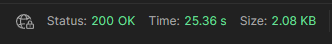
\includegraphics[width=0.5\textwidth]{resources/ch4/time/1-postman.png}
	\caption{\textit{Response time} dari Postman untuk kasus SI1}
	\label{time_p_1}
\end{figure}

\begin{figure}[!htb]
	\centering
	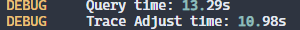
\includegraphics[width=0.5\textwidth]{resources/ch4/time/1-log.png}
	\caption{Pencatatan waktu fungsi kasus SI1}
	\label{time_l_1}
\end{figure}



\subsection{Analisis Hasil Pengujian}
Dari semua kasus pengujian, hasil yang didapatkan dari pengujian akan bergantung pada nilai signifikan yang digunakan untuk menguji masing-masing kasus. Terdapat 3 nilai signifikan yang penulis gunakan untuk melakukan pengujian yaitu 0,1, 0,005, dan 0,001 dengan maksud menguji sensitivitas dari algoritma pendeteksian regresi diberikan nilai signifikan yang berbeda-beda. Hasilnya adalah pengujian dengan nilai signifikan 0,1 berhasil mendeteksi dan menganalisis penyebab regresi dengan benar pada semua kasus uji, namun pada pengujian dengan nilai signifikan 0,05 dan 0,001 kasus SI1 tidak terdeteksi sebagai regresi.

Gambar \ref{result_log_1} menunjukkan \textit{log} yang didapatkan dari kasus SI1 dengan nilai signifikan 0,05.


Dari hasil pengujian, pada level signifikan 0,01 semua kasus regresi dapat dideteksi 

Dari tujuh kasus uji, kasus SI1 sampai SI7, yang menyimulasikan terjadinya regresi akibat perubahan di level kode, hanya satu kasus, yaitu kasus SI1, yang regresi tidak dapat terdeteteksi oleh PRA Engine. Selebihnya, dari enam kasus lainnya, PRA Engine dapat mendeteksi terjadinya regresi dan juga dapat menentukan kandidat operasi sumber terjadinya regresi dengan menghitung selisih \textit{latency} antara data \textit{trace} \textit{baseline} dan periodikal. 

\begin{figure}[!htb]
	\centering
	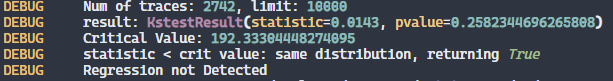
\includegraphics[width=1\textwidth]{resources/ch4/log/1-log.png}
	\caption{\textit{Log} hasil pengujian kasus SI1 dengan alpha 0,05}
	\label{result_log_1}
\end{figure}

Gambar \ref{result_log_1} merupakan \textit{log} yang didapatkan dari kasus SI1 yang menampilkan hasil tes statistik K-S. Nilai \texttt{p-value} yang didapatkan dari hasil tes lebih besar dari nilai signifikan yaitu 0.05 dan juga nilai \texttt{statistic} lebih kecil dari nilai \texttt{critical value} sehingga hipotesis $h_{0}$ tidak dapat ditolak dan PRA Engine menginterpretasikan bahwa data \textit{latency} dari kasus SI1 berasal dari distribusi yang sama dengan data \textit{latency} \textit{baseline}. 

Dari analisis hasil kasus SI1 dapat terlihat bahwa algoritma tidak dapat mendeteksi terjadinya regresi jika tidak terdapat perbedaan signifikan antara kedua sampel data seperti pada kasus SI1 yang hanya menyimulasikan penambahan \textit{latency} sebesar 100ms pada satu buah operasi. Sementara pada kasus selanjutnya, yaitu kasus SI2 dengan penambahan \textit{latency} sebesar 250ms, PRA Engine dapat mendeteksi bahwa data \textit{latency} periodikal berasal dari distribusi yang berbeda dengan data \textit{latency} \textit{baseline} sehingga PRA Engine dapat mendeteksi terjadinya regresi.

Sementara pada kasus-kasus yang menyimulasikan perubahan dari eksternal, yaitu kasus SE1 sampai SE4, PRA Engine juga dapat mendeteksi terjadinya regresi karena algoritma dapat menentukan bahwa data \textit{latency} pada kasus-kasus tersebut berasal dari distribusi yang berbeda dari data \textit{latency} \textit{baseline}.

Dapat disimpulkan bahwa algoritma belum dapat menentukan apakah regresi yang terjadi diakibatkan oleh perubahan yang terjadi pada level aplikasi ataupun perubahan yang terjadi di luar aplikasi seperti peningkatan jumlah pengguna ataupun peningkatan \textit{load} pada sebagian operasi. Namun jika dari analisis \textit{critical path} dapat terlihat selisih \textit{latency} dari operasi yang melebihi \textit{threshold} tertentu dapat menjadi indikasi bahwa regresi yang terjadi diakibatkan oleh perubahan di level aplikasi. Sebaliknya, jika analisis \textit{critical path} tidak dapat menentukan operasi yang menjadi kandidat penyebab regresi karena selisihnya tidak lebih besar daripada \textit{threshold}, seperti yang terlihat pada gambar \ref{result_json_8}, maka dapat menjadi indikasi bahwa regresi yang terdeteksi diakibatkan oleh perubahan yang disebabkan oleh faktor eksternal.

\chapter{Kesimpulan dan Saran}
Bab ini berisi hal-hal yang dapat disimpulkan dari pelaksanaan Tugas Akhir ini. Bab ini juga mencakup saran untuk pengembangan Tugas Akhir ini di masa mendatang.

\section{Kesimpulan}
Berdasarkan hasil pengembangan dan pengujian sistem \textit{Performance Regression Analysis} (PRA) yang telah dilakukan. Berikut ini adalah kesimpulan yang diperoleh.
\begin{enumerate}
	\item Telah berhasil dilakukan pendeteksian regresi pada kinerja aplikasi berbasis microservice menggunakan \textit{engine} PRA.
	\item Telah berhasil dilakukan analisis untuk menentukan akar penyebab regresi pada aplikasi berbasis microservice.
	\item Pendeteksian regresi dapat dilakukan dengan menggunakan statistik Kolmogorov-Smirnov dengan membandingkan distribusi kumulatif antara dua sampel \textit{latency} service-service yang terdapat pada aplikasi berbasis microservice. Statistik Kolmogorov-Smirnov akan mengajukan hipotesis h0 $a_{ij}$
	Dari statistik Kolmogorov-Smirnov yang diperoleh, jika nilai statistik melebihi nilai kritis maka akan ditolak 
	Statistik Kolmogorov-Smirnov akan dihitung berdasarkan jumlah sampel latency masing-masing dan akan dibandingkan nilai nya dengan 
	
	 \item Konflik pada kolaborasi dapat ditangani dengan baik oleh sistem pada EtherCalc sehingga penanganan konflik tidak perlu dibuat kembali.	
	\item Data yang akan dimasukkan ke basis data penyimpanan berhasil divalidasi menggunakan fitur yang dibuat dengan tiga tipe validasi yakni tipe data, domain data, dan relasi data.
	\item Identifikasi tabel pada suatu \textit{sheet} dapat dilakukan dengan menggunakan algoritma kNN dengan mencari kedekatan antar sel. Identifikasi label suatu baris pada tabel dapat dilakukan dengan teknik \textit{frame finder} dengan membagi label menjadi empat jenis yakni \textit{title}, \textit{data}, \textit{header}, dan \textit{footer}. Jika teknik \textit{frame finder} tidak berhasil menemukan label dan data, maka pengguna dapat memasukkan \textit{metadata table} secara manual dan mengubahnya sesuai dengan keinginan pengguna.
	\item Penggabungan data antar \textit{spreadsheet} dapat dilakukan dengan fitur yang dibuat dan dapat digabungkan secara horizontal, vertikal, maupun gabungan keduanya. Data pada \textit{spreadsheet} berhasil dimasukkan ke dalam basis data yang ditentukan sesuai dengan \textit{metadata table} yang telah dibuat pengguna maupun hasil pencarian otomatis dari algoritma \textit{frame finder}.
	\item Alur kerja pengumpulan data berubah sehingga dapat diusulkan alur kerja baru dimana \textit{versioning} dilakukan oleh aplikasi EtherCalc karena seluruh data berada pada satu tempat menggunakan mekanisme penyimpanan oleh EtherCalc. Pada saat pengumpulan data dari berbagai \textit{spreadsheet} dapat dilakukan menggunakan aplikasi yang sama yakni EtherCalc, sehingga pada alur kerja yang diusulkan, pengumpulan data tidak memerlukan bantuan aplikasi lain ataupun manual. Hasil akhir dari pengumpulan data merupakan data pada basis data sehingga data mudah diolah, ditampilkan, maupun diubah menggunakan banyak aplikasi yang tersedia.
\end{enumerate}

\section{Saran}
Saran yang dapat diberikan untuk pengembangan di masa mendatang adalah sebagai berikut:
\begin{enumerate}
	\item Pada pembangunan selanjutnya dapat ditambahkan penanganan kasus penggunaan \textit{spreadsheet} selain \textit{data frame} dan relasi.
	\item Penambahan data pembelajaran untuk identifikasi label baris dapat dilakukan sehingga akan memperbaiki hasil identifikasi otomatis. Pada pengembangan selanjutnya dapat ditambahkan \textit{feedback} dari pengguna sebagai data pembelajaran.
	\item Menambahkan fungsionalitas yakni memperbolehkan kolom \textit{key} yang tidak hanya satu pada \textit{metadata table}.
	\item Pengembangan fitur validasi, contohnya adalah menambahkan jenis validasi contohnya validasi masukan berbentuk formula. Di samping itu, dapat ditambahkan jenis validasi pada validasi tipe seperti tipe tanggal. Dapat juga penambahan fitur pada validasi domain seperti atribut yang dapat menerima tidak hanya satu aturan validasi domain.
	\item Penanganan jenis tabel dengan \textit{header} yang berada di kiri dan kanan data mungkin dapat dikembangkan menggunakan teknik \textit{transpose}.

\end{enumerate}
%----------------------------------------------------------------%

% Daftar pustaka
% Bibliography to Daftar Pustaka
\renewcommand{\bibname}{Daftar Pustaka}
\cleardoublepage
\phantomsection
\addcontentsline{toc}{chapter}{DAFTAR PUSTAKA}
%\printbibliography
%\bibliography{references}
%ZCZC RMS 202107023
%\bibstyle{apa}
\bibliography{references}
\bibliographystyle{apalike}

\backmatter
% Index
\appendix
\addtocontents{toc}{\protect\setcounter{tocdepth}{2}}

\cleardoublepage
\phantomsection
%\part*{Lampiran}
%\addcontentsline{toc}{part}{LAMPIRAN}

% Setting judul appendix
\chapterfont{\Large}
\titleformat{\chapter}[hang]
{\Large\bfseries}
{\chaptertitlename\ \thechapter.\ }{0pt}
{\Large\bfseries}
\titlespacing*{\chapter}{0pt}{-25pt}{10pt}

\chapter{Lampiran A. Tangkapan Layar Hasil Pengujian Regresi}
\label{lampiran_a}

\begin{figure}[!htb]
	\centering
	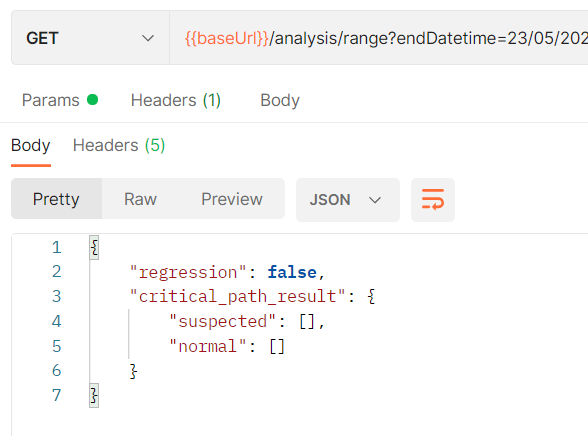
\includegraphics[width=0.75\textwidth]{resources/ch4/json/1-new.png}
	\caption{\textit{Response} JSON hasil pengujian kasus \textbf{SI1}}
	\label{result_json_1}
\end{figure}

%\begin{figure}[!htb]
%	\centering
%	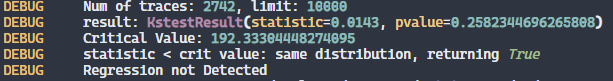
\includegraphics[width=1\textwidth]{resources/ch4/log/1-log.png}
%	\caption{\textit{Log} hasil pengujian kasus SI1}
%	\label{result_log_1}
%\end{figure}

\begin{figure}[!htb]
	\centering
	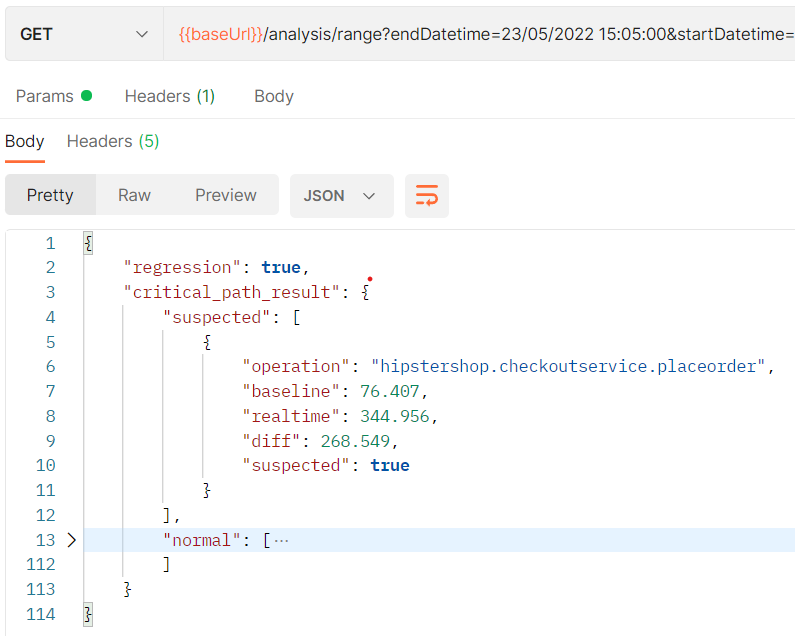
\includegraphics[width=0.75\textwidth]{resources/ch4/json/2-new.png}
	\caption{\textit{Response} JSON hasil pengujian kasus \textbf{SI2}}
	\label{result_json_2}
\end{figure}

%\begin{figure}[!htb]
%	\centering
%	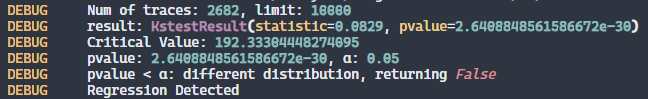
\includegraphics[width=1\textwidth]{resources/ch4/log/2-log.png}
%	\caption{\textit{Log} hasil pengujian kasus SI2}
%	\label{result_log_2}
%\end{figure}

\begin{figure}[!htb]
	\centering
	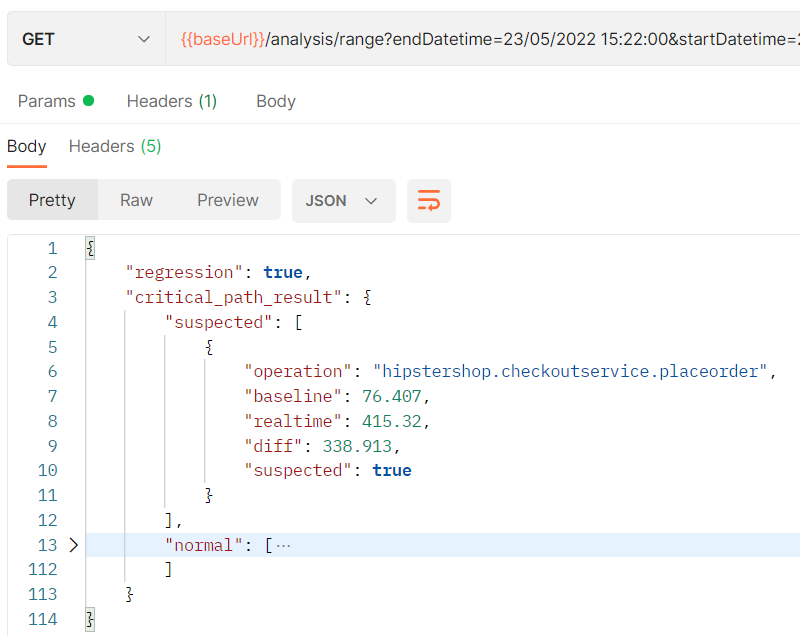
\includegraphics[width=0.75\textwidth]{resources/ch4/json/3-new.png}
	\caption{\textit{Response} JSON hasil pengujian kasus \textbf{SI3}}
	\label{result_json_3}
\end{figure}

%\begin{figure}[!htb]
%	\centering
%	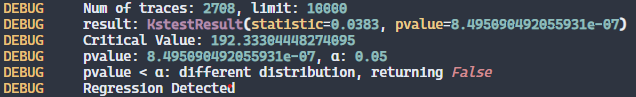
\includegraphics[width=1\textwidth]{resources/ch4/log/3-log.png}
%	\caption{\textit{Log} hasil pengujian kasus SI3}
%	\label{result_log_3}
%\end{figure}
%\pagebreak

\begin{figure}[!htb]
	\centering
	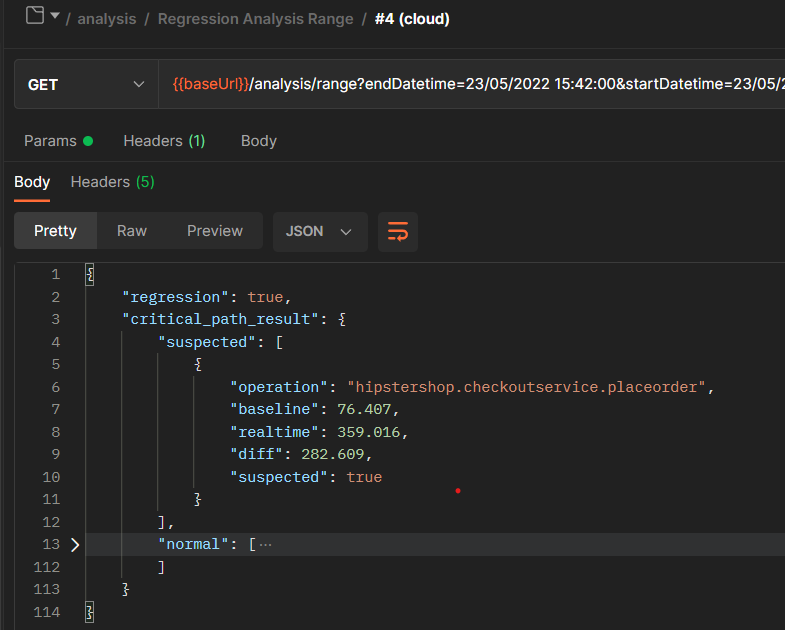
\includegraphics[width=0.75\textwidth]{resources/ch4/json/4.png}
	\caption{\textit{Response} JSON hasil pengujian kasus \textbf{SI4}}
	\label{result_json_4}
\end{figure}

%\begin{figure}[!htb]
%	\centering
%	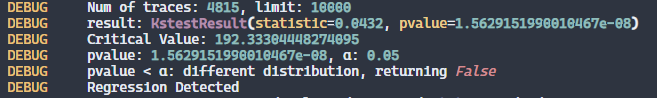
\includegraphics[width=1\textwidth]{resources/ch4/log/4-log.png}
%	\caption{\textit{Log} hasil pengujian kasus SI4}
%	\label{result_log_4}
%\end{figure}

\begin{figure}[!htb]
	\centering
	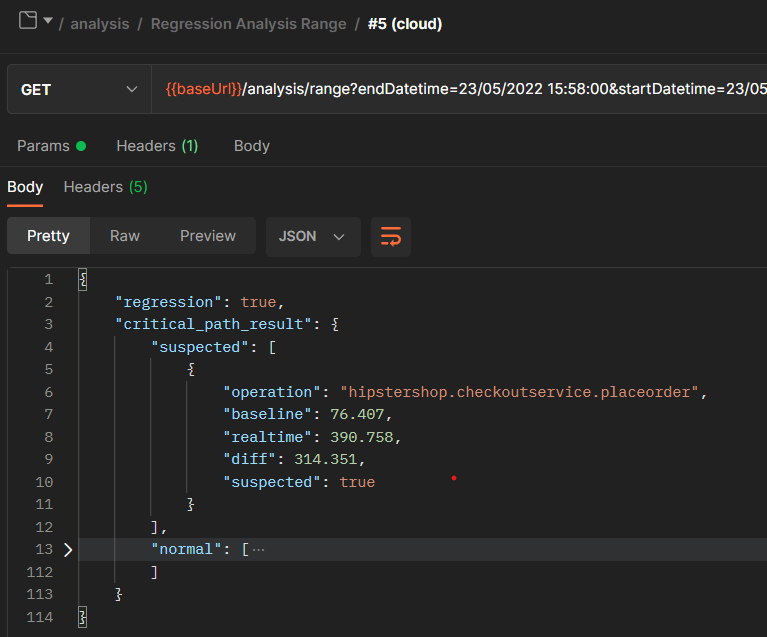
\includegraphics[width=0.75\textwidth]{resources/ch4/json/5.png}
	\caption{\textit{Response} JSON hasil pengujian kasus \textbf{SI5}}
	\label{result_json_5}
\end{figure}

%\begin{figure}[!htb]
%	\centering
%	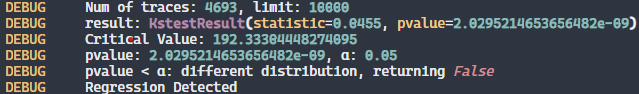
\includegraphics[width=1\textwidth]{resources/ch4/log/5-log.png}
%	\caption{\textit{Log} hasil pengujian kasus \textbf{SI5}}
%	\label{result_log_5}
%\end{figure}

\begin{figure}[!htb]
	\centering
	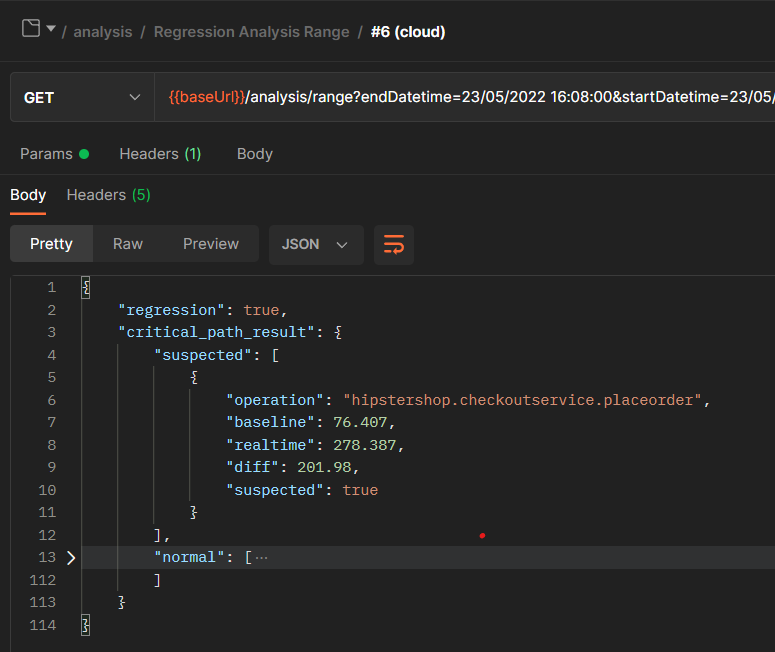
\includegraphics[width=0.75\textwidth]{resources/ch4/json/6.png}
	\caption{\textit{Response} JSON hasil pengujian kasus \textbf{SI6}}
	\label{result_json_6}
\end{figure}

%\begin{figure}[!htb]
%	\centering
%	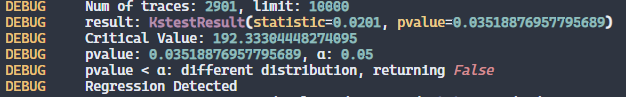
\includegraphics[width=1\textwidth]{resources/ch4/log/6-log.png}
%	\caption{\textit{Log} hasil pengujian kasus SI6}
%	\label{result_log_6}
%\end{figure}
%\pagebreak

\begin{figure}[!htb]
	\centering
	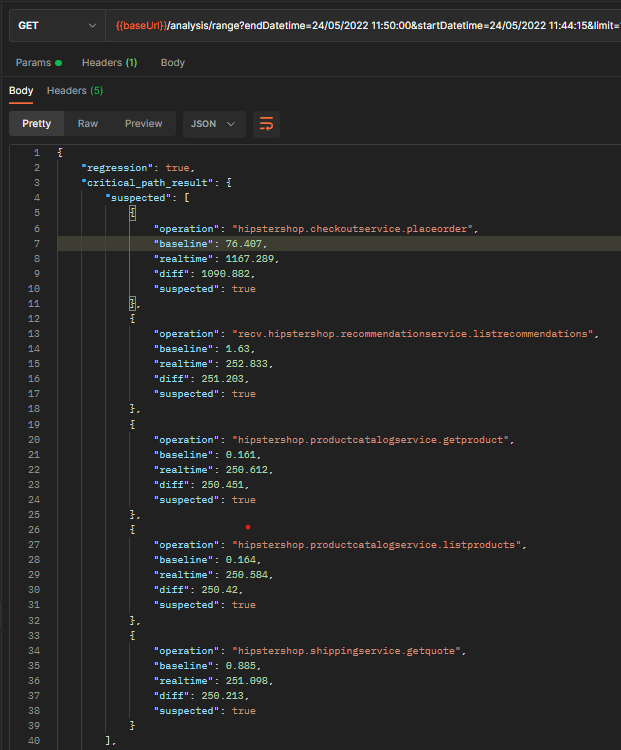
\includegraphics[width=0.75\textwidth]{resources/ch4/json/7.png}
	\caption{\textit{Response} JSON hasil pengujian kasus \textbf{SI7}}
	\label{result_json_7}
\end{figure}
%
%\begin{figure}[!htb]
%	\centering
%	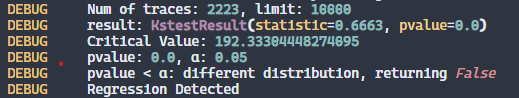
\includegraphics[width=1\textwidth]{resources/ch4/log/7-log.png}
%	\caption{\textit{Log} hasil pengujian kasus SI7}
%	\label{result_log_7}
%\end{figure}

\begin{figure}[!htb]
	\centering
	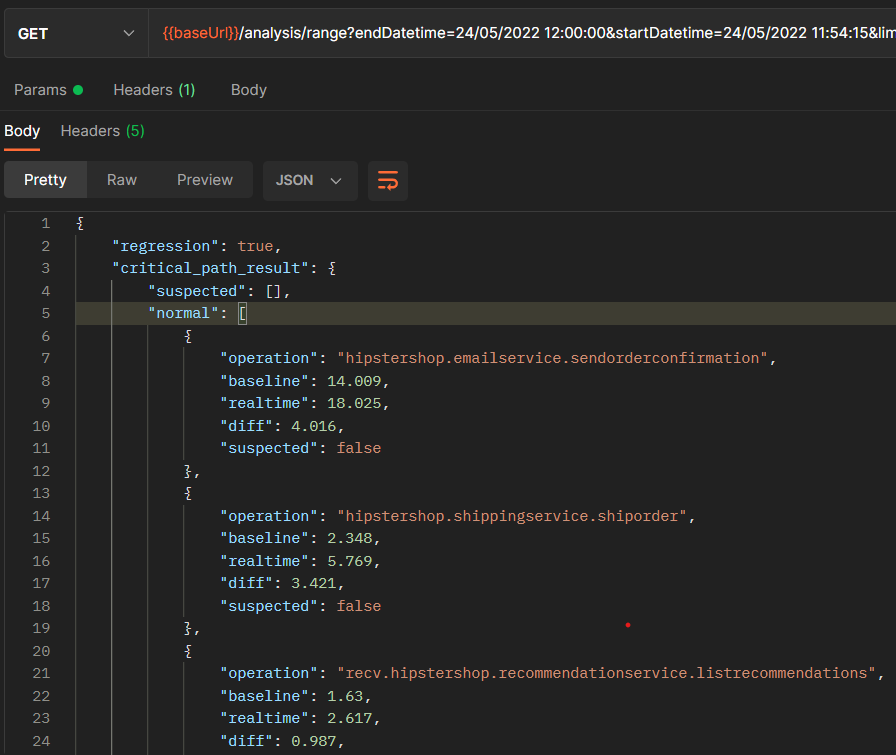
\includegraphics[width=0.75\textwidth]{resources/ch4/json/8.png}
	\caption{\textit{Response} JSON hasil pengujian kasus \textbf{SE1}}
	\label{result_json_8}
\end{figure}

%\begin{figure}[!htb]
%	\centering
%	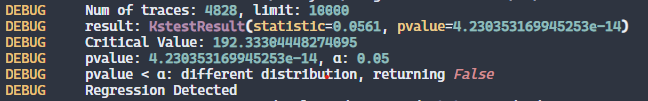
\includegraphics[width=1\textwidth]{resources/ch4/log/8-log.png}
%	\caption{\textit{Log} hasil pengujian kasus SE1}
%	\label{result_log_8}
%\end{figure}

\begin{figure}[!htb]
	\centering
	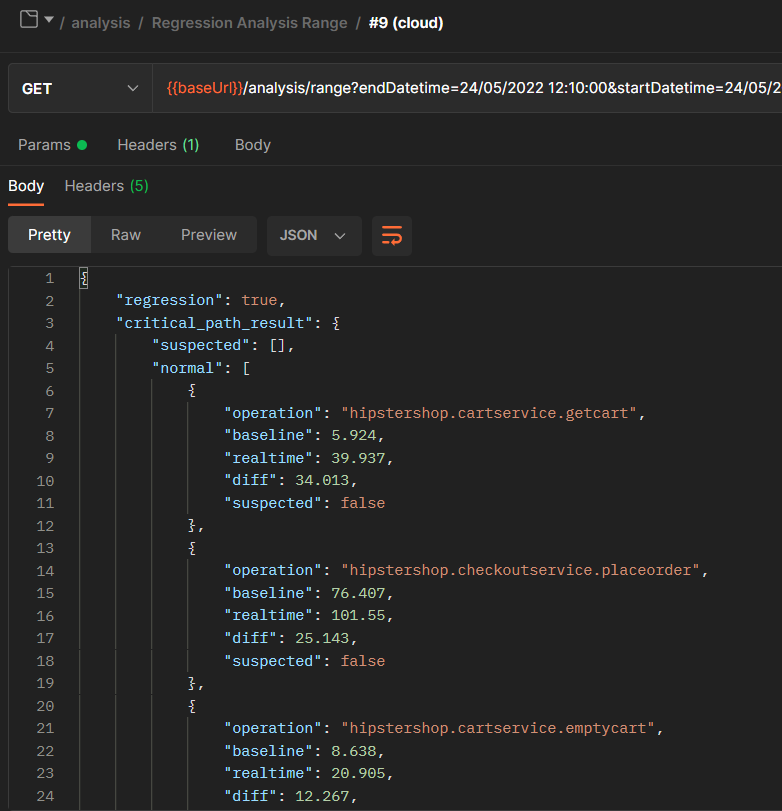
\includegraphics[width=0.75\textwidth]{resources/ch4/json/9.png}
	\caption{\textit{Response} JSON hasil pengujian kasus \textbf{SE2}}
	\label{result_json_9}
\end{figure}

%\begin{figure}[!htb]
%	\centering
%	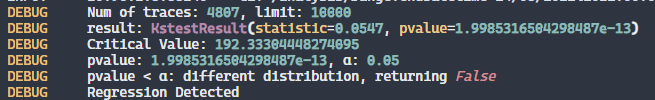
\includegraphics[width=1\textwidth]{resources/ch4/log/9-log.png}
%	\caption{\textit{Log} hasil pengujian kasus SE2}
%	\label{result_log_9}
%\end{figure}

\begin{figure}[!htb]
	\centering
	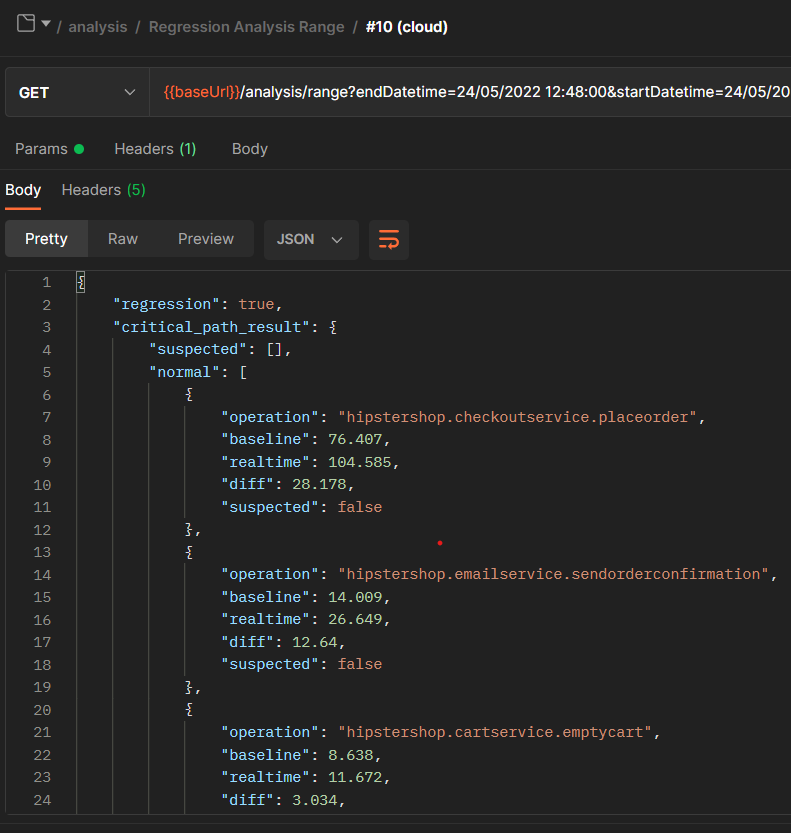
\includegraphics[width=0.75\textwidth]{resources/ch4/json/10.png}
	\caption{\textit{Response} JSON hasil pengujian kasus \textbf{SE3}}
	\label{result_json_10}
\end{figure}
%\begin{figure}[!htb]
%	\centering
%	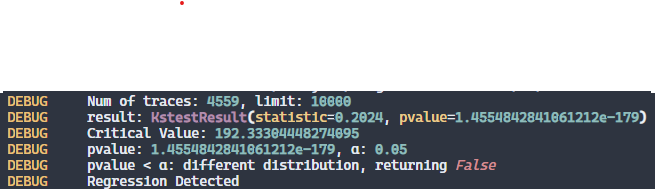
\includegraphics[width=1\textwidth]{resources/ch4/log/10-log.png}
%	\caption{\textit{Log} hasil pengujian kasus SE3}
%	\label{result_log_10}
%\end{figure}

\begin{figure}[!htb]
	\centering
	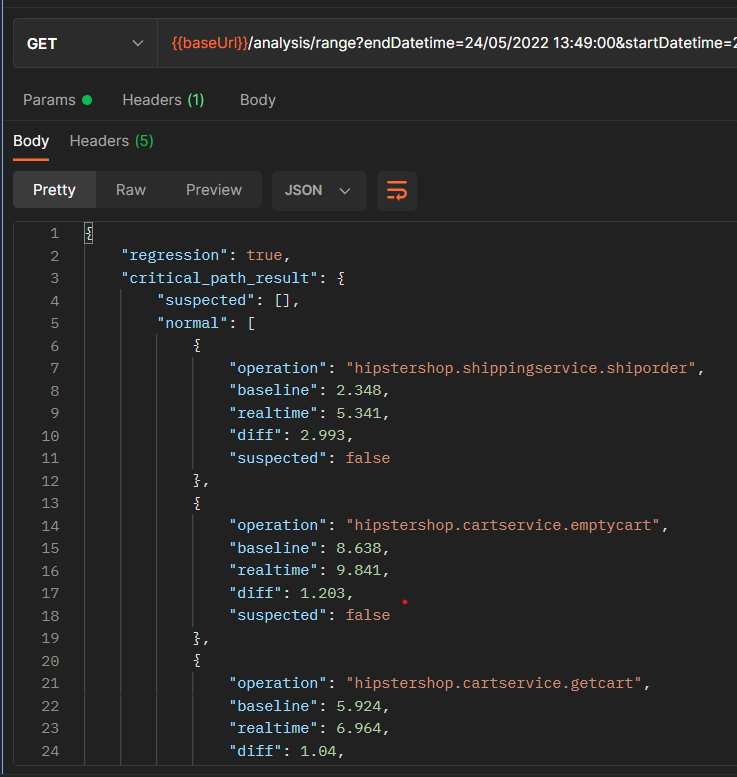
\includegraphics[width=0.75\textwidth]{resources/ch4/json/11.png}
	\caption{\textit{Response} JSON hasil pengujian kasus \textbf{SE4}}
	\label{result_json_9}
\end{figure}

%\begin{figure}[!htb]
%	\centering
%	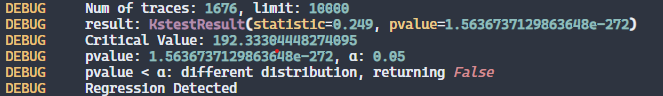
\includegraphics[width=1\textwidth]{resources/ch4/log/11-log.png}
%	\caption{\textit{Log} hasil pengujian kasus SE4}
%	\label{result_log_11}
%\end{figure}
\chapter{Lampiran B. Tabel dan Tangkapan Layar Hasil Pengujian Kinerja}
\label{lampiran_b}

% Please add the following required packages to your document preamble:
% \usepackage[table,xcdraw]{xcolor}
% If you use beamer only pass "xcolor=table" option, i.e. \documentclass[xcolor=table]{beamer}
\begin{table}[]
	\caption{Tabel hasil pengujian kinerja}
	\centering
	\begin{tabular}{|l|c|c|}
		\hline
		\rowcolor[HTML]{6434FC} 
		{\color[HTML]{FFFFFF} ID} &
		\multicolumn{1}{l|}{\cellcolor[HTML]{6434FC}{\color[HTML]{FFFFFF} CPU (vCPU)}} &
		\multicolumn{1}{l|}{\cellcolor[HTML]{6434FC}{\color[HTML]{FFFFFF} Memory (MiB)}} \\ \hline
		\textbf{SI1}     & 0,042 & 137,82  \\ \hline
		\textbf{SI2}     & 0,043 & 128,71  \\ \hline
		\textbf{SI3}     & 0,04  & 131,55  \\ \hline
		\textbf{SI4}     & 0,045 & 146,6   \\ \hline
		\textbf{SI5}     & 0,046 & 153,61  \\ \hline
		\textbf{SI6}     & 0,047 & 152,71  \\ \hline
		\textbf{SI7}     & 0,048 & 152,71  \\ \hline
		\textbf{SE1}     & 0,049 & 168,8   \\ \hline
		\textbf{SE2}     & 0,05  & 183,68  \\ \hline
		\textbf{SE3}     & 0,051 & 176,59  \\ \hline
		\textbf{SE4}     & 0,052 & 165,75  \\ \hline
		\textbf{Average} & 0,046 & 154,411 \\ \hline
		\textbf{STD}     & 0,038 & 17,916  \\ \hline
	\end{tabular}
\end{table}

\begin{figure}[!htb]
	\centering
	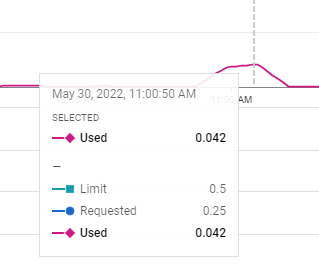
\includegraphics[width=0.5\textwidth]{resources/ch4/resource/1-cpu.png}
	\caption{Penggunaan CPU pada kasus \textbf{SI1}}
	\label{result_cpu_1}
\end{figure}

\begin{figure}[!htb]
	\centering
	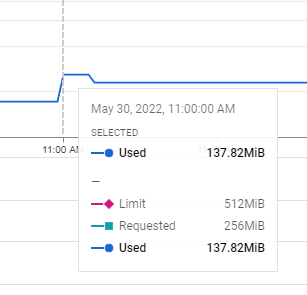
\includegraphics[width=0.5\textwidth]{resources/ch4/resource/1-mem.png}
	\caption{Penggunaan Memory pada kasus \textbf{SI1}}
	\label{result_mem_1}
\end{figure}

\begin{figure}[!htb]
	\centering
	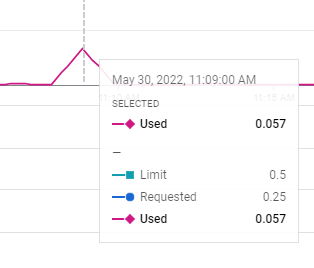
\includegraphics[width=0.5\textwidth]{resources/ch4/resource/2-cpu.png}
	\caption{Penggunaan CPU pada kasus \textbf{SI2}}
	\label{result_cpu_2}
\end{figure}

\begin{figure}[!htb]
	\centering
	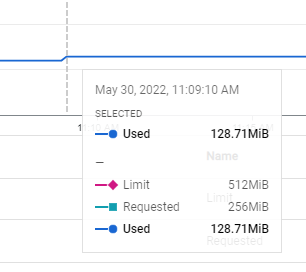
\includegraphics[width=0.5\textwidth]{resources/ch4/resource/2-mem.png}
	\caption{Penggunaan Memory pada kasus \textbf{SI2}}
	\label{result_mem_2}
\end{figure}

\begin{figure}[!htb]
	\centering
	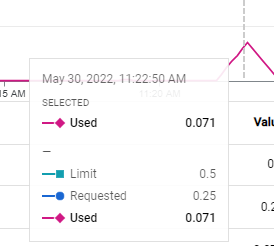
\includegraphics[width=0.5\textwidth]{resources/ch4/resource/3-cpu.png}
	\caption{Penggunaan CPU pada kasus \textbf{SI3}}
	\label{result_cpu_3}
\end{figure}

\begin{figure}[!htb]
	\centering
	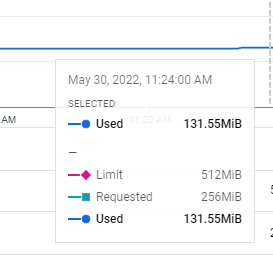
\includegraphics[width=0.5\textwidth]{resources/ch4/resource/3-mem.png}
	\caption{Penggunaan Memory pada kasus \textbf{SI3}}
	\label{result_mem_3}
\end{figure}

\begin{figure}[!htb]
	\centering
	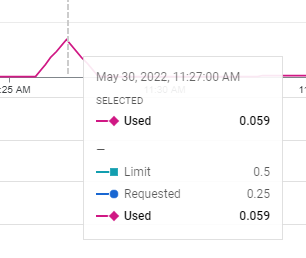
\includegraphics[width=0.5\textwidth]{resources/ch4/resource/4-cpu.png}
	\caption{Penggunaan CPU pada kasus \textbf{SI4}}
	\label{result_cpu_4}
\end{figure}

\begin{figure}[!htb]
	\centering
	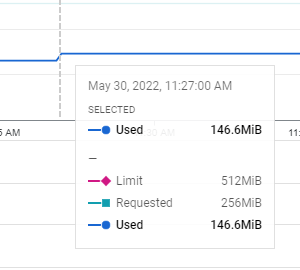
\includegraphics[width=0.5\textwidth]{resources/ch4/resource/4-mem.png}
	\caption{Penggunaan Memory pada kasus \textbf{SI4}}
	\label{result_mem_4}
\end{figure}

\begin{figure}[!htb]
	\centering
	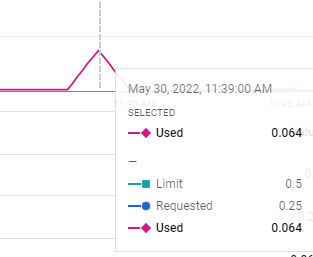
\includegraphics[width=0.5\textwidth]{resources/ch4/resource/5-cpu.png}
	\caption{Penggunaan CPU pada kasus \textbf{SI5}}
	\label{result_cpu_5}
\end{figure}

\begin{figure}[!htb]
	\centering
	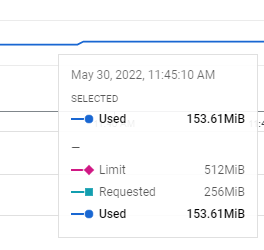
\includegraphics[width=0.5\textwidth]{resources/ch4/resource/5-mem.png}
	\caption{Penggunaan Memory pada kasus \textbf{SI5}}
	\label{result_mem_5}
\end{figure}

\begin{figure}[!htb]
	\centering
	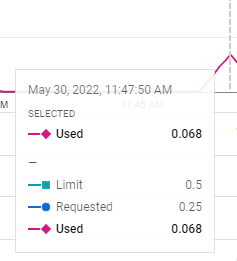
\includegraphics[width=0.5\textwidth]{resources/ch4/resource/6-cpu.png}
	\caption{Penggunaan CPU pada kasus \textbf{SI6}}
	\label{result_cpu_6}
\end{figure}

\begin{figure}[!htb]
	\centering
	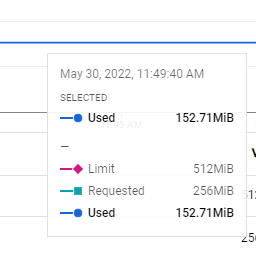
\includegraphics[width=0.5\textwidth]{resources/ch4/resource/6-mem.png}
	\caption{Penggunaan Memory pada kasus \textbf{SI6}}
	\label{result_mem_6}
\end{figure}

\begin{figure}[!htb]
	\centering
	\includegraphics[width=0.5\textwidth]{resources/ch4/resource/7-cpu.png}
	\caption{Penggunaan CPU pada kasus \textbf{SI7}}
	\label{result_cpu_7}
\end{figure}

\begin{figure}[!htb]
	\centering
	\includegraphics[width=0.5\textwidth]{resources/ch4/resource/7-mem.png}
	\caption{Penggunaan Memory pada kasus \textbf{SI7}}
	\label{result_mem_7}
\end{figure}

\begin{figure}[!htb]
	\centering
	\includegraphics[width=0.5\textwidth]{resources/ch4/resource/8-cpu.png}
	\caption{Penggunaan CPU pada kasus \textbf{SE1}}
	\label{result_cpu_8}
\end{figure}

\begin{figure}[!htb]
	\centering
	\includegraphics[width=0.5\textwidth]{resources/ch4/resource/8-mem.png}
	\caption{Penggunaan Memory pada kasus \textbf{SE1}}
	\label{result_mem_8}
\end{figure}

\begin{figure}[!htb]
	\centering
	\includegraphics[width=0.5\textwidth]{resources/ch4/resource/9-cpu.png}
	\caption{Penggunaan CPU pada kasus \textbf{SE2}}
	\label{result_cpu_9}
\end{figure}

\begin{figure}[!htb]
	\centering
	\includegraphics[width=0.5\textwidth]{resources/ch4/resource/9-mem.png}
	\caption{Penggunaan Memory pada kasus \textbf{SE2}}
	\label{result_mem_9}
\end{figure}

\begin{figure}[!htb]
	\centering
	\includegraphics[width=0.5\textwidth]{resources/ch4/resource/10-cpu.png}
	\caption{Penggunaan CPU pada kasus \textbf{SE3}}
	\label{result_cpu_10}
\end{figure}

\begin{figure}[!htb]
	\centering
	\includegraphics[width=0.5\textwidth]{resources/ch4/resource/10-mem.png}
	\caption{Penggunaan Memory pada kasus \textbf{SE3}}
	\label{result_mem_10}
\end{figure}

\begin{figure}[!htb]
	\centering
	\includegraphics[width=0.5\textwidth]{resources/ch4/resource/11-cpu.png}
	\caption{Penggunaan CPU pada kasus \textbf{SE4}}
	\label{result_cpu_11}
\end{figure}

\begin{figure}[!htb]
	\centering
	\includegraphics[width=0.5\textwidth]{resources/ch4/resource/11-mem.png}
	\caption{Penggunaan Memory pada kasus \textbf{SE4}}
	\label{result_mem_11}
\end{figure}

\end{document}

